%%%%%%%%%%%%%%%%%%%%%%%%%%%%%%%%%%%%%%%%%%%%%%%%%%%%%%%%%%%%%%%%%%%%%%%%%%%%%%%%
%% Plantilla de memoria en LaTeX para TFG/TFM - Universidad Rey Juan Carlos
%%
%% Por Gregorio Robles <grex arroba gsyc.urjc.es>
%%     Felipe Ortega   <felipe.ortega@urjc.es>
%%     Grupo de Sistemas y Comunicaciones (GSyC)
%%     Escuela Técnica Superior de Ingenieros de Telecomunicación
%%     Universidad Rey Juan Carlos
%%
%% (Muchas ideas tomadas de Internet, colegas del GSyC, antiguos alumnos...
%%  etc. Muchas gracias a todos)
%%
%% La última versión de esta plantilla está siempre disponible en:
%%     https://github.com/glimmerphoenix/plantilla-memoria
%%
%% - Ejecución en sistema local:
%% Para obtener el documento en PDF, ejecuta en la shell:
%%   make
%%
%% A diferencia de la anterior versión, que usaba la herramienta pdfLaTeX 
%% para compilar el documento, esta nueva versión de la plantilla usa
%% XeLaTeX. Es un compilador más moderno que, entre otras mejoras, incluye
%% soporte nativo para caracteres con codificación UTF-8, traducción políglota
%% de referencias (usando Biblatex) y soporte para fuentes OTF. Esta última
%% característic permite, por ejemplo, insertar iconos de la colección 
%% Fontawesome en el texto.
%%
%% XeLaTeX viene ya incluido en todas las distribuciones modernas de LaTeX.
%%
%% - Edición y ejecución en línea: 
%% Puedes descargar y subir la plantilla a
%% Overleaf, un editor de LaTeX colaborativo en línea. Overleaf ya tiene
%% instalados todos los paquetes LaTeX y otras dependencias software para
%% que esta plantilla compile correctamente.
%%
%% IMPORTANTE: Si compilas este documento en Overleaf, recuerda cambiar
%% la configuración (botón "Menu" en la esquina superior izquierda de la interfaz)
%% y elegir la opción Compiler --> XeLaTeX. En caso contrario no funcionará.
%%
%% - Nota: las imágenes deben ir en PNG, JPG, EPS o PDF. También se pueden usar
%% imágenes en otros formatos con algunos cambios en el preámbulo del documento.

%%%%%%%%%%%%%%%%%%%%%%%%%%%%%%%%%%%%%%%%%%%%%%%%%%%%%%%%%%%%%%%%%%%%%%%%%%%%%%%%

\documentclass[a4paper, 12pt]{book}

%%-- Geometría principal (dejar activada la siguiente línea en la versión final)
\usepackage[a4paper, left=2.5cm, right=2.5cm, top=3cm, bottom=3cm]{geometry}

%% Ruptura de página y línea
\sloppy
\clubpenalty= 10000
\widowpenalty=10000
\brokenpenalty=10000

%%-- Activar esta línea y comentar la anterior en modo borrador, para comentarios al margen
%\usepackage[a4paper, left=2.5cm, right=2.5cm, top=3cm, bottom=3cm, marginparwidth=60pt]{geometry}
\usepackage{multirow}
\usepackage{diagbox}
\usepackage{adjustbox}
\usepackage{eurosym}
\usepackage{array}
    \newcolumntype{P}[1]{>{\centering\arraybackslash}p{#1}}

%%-- Hay que cargarlo antes que las traducciones
\usepackage{listing}                    % Listados de código
\usepackage{listings} 

% Traducciones en XeLaTeX
\usepackage{polyglossia}
\setmainlanguage{spanish}    % Comenta esta línea si tu memoria es en inglés

% Traducciones particulares para español
% Caption tablas
\gappto\captionsspanish{
	\def\tablename{Tabla}
	\def\listingscaption{Código}
	\def\refname{Bibliografía}
	\def\appendixname{Apéndice}
	\def\listtablename{Índice de tablas}
	\def\listingname{Código}
	\def\listlistingname{Índice de fragmentos de código}
}

%% Tipografía y estilos
\usepackage[OT1]{fontenc}               % Keeps eulervm happy about accents encoding

% Símbolos y fuentes matemáticas elegantes: Euler virtual math fonts
% ¡Importante! Carga siempre las fuentes math AMS Euler ANTES QUE fontspec
\usepackage{amsmath}
\usepackage{amssymb}
\usepackage[OT1,euler-digits,euler-hat-accent,small]{eulervm}

% En XeLaTeX las fuentes se especifican con fontspec
\usepackage{fontspec}
\defaultfontfeatures{Scale=MatchLowercase, Ligatures=TeX}     % Default option in font config

% Fix para fuentes usadas con operadores y \mathrm
\DeclareSymbolFont{operators}{\encodingdefault}{\familydefault}{m}{n}

% Configura la fuente principal (serif): MinionPro
\setmainfont[Scale=0.96]{TeX Gyre Pagella}
% Configura la fuente sans-serif (\sffamily)
\setsansfont[Scale=MatchLowercase]{Lato}
% Configura la fuente para letra monoespaciada: Source Code Pro, escala 0.85
\setmonofont[Scale=0.85]{Source Code Pro}

%%-- Familias de fuentes específicas
%%-- Se pueden definir etiquetas para familias de fuentes personalizadas
%%-- que luego puedes emplear para cambiar el formato de una parte de texto
%%-- Ejemplo:
% \newfontfamily{\myriadprocond}{Myriad Pro Semibold Condensed.otf}

%%-- Opciones de interlineado y espacios
\linespread{1.07}                   % Aumentar interlineado para fuentes tipo Palatino
\setlength{\parskip}{\baselineskip} % Separar párrafos con línea en blanco

%%-- Hipervínculos
\usepackage{url}

%%-- Gráficos y tablas
\PassOptionsToPackage{
    dvipdfmx,usenames,dvipsnames,
    x11names,table}{xcolor}             % Definiciones de colores
\PassOptionsToPackage{xetex}{graphicx}

\usepackage{subfig}                     % Subfiguras
\usepackage{pgf}
\usepackage{svg}                        % Integración de imágenes en formato SVG
\usepackage{float}                      % H para posicionar figuras
\usepackage{booktabs}                   % Already loads package xcolor
\usepackage{multicol}                   % multiple column layout facilities
\usepackage{colortbl}                   % For coloured tables
\usepackage{comment}

%%-- Bibliografía con Biblatex y Biber
% Más info:
% https://www.overleaf.com/learn/latex/Biblatex_bibliography_styles
% https://www.overleaf.com/learn/latex/biblatex_citation_styles
\usepackage[
    backend=biber,
    style=numeric,
    sorting=nty
    ]{biblatex}
\addbibresource{memoria.bib}
\DeclareFieldFormat{url}{\mkbibacro{URL}\addcolon\nobreakspace\url{#1}}
%\usepackage[nottoc, notlot, notlof, notindex]{tocbibind} %% Opciones de índice

%%-- Matemáticas e ingeniería
% El paquete units permite mostrar unidades correctamente
% Permite escribir unidades con espaciado y estilo de fuente correctos
\usepackage[ugly]{units}         
% Ejemplo de uso: $\unit[100]{m}$ or $\unitfrac[100]{m}{s}$
% Entornos matemáticos
\newtheorem{theorem}{Theorem}

% Paquetes adicionales
\usepackage{url}                        %% Gestión correcta de enlaces
\usepackage{float}                      %% H para posicionar figuras
\usepackage[nottoc, notlot, notlof, notindex]{tocbibind}    %% Opciones de índice
\usepackage{metalogo}                   %% Múltiples logos para XeLaTeX

% Fuentes especiales y glifos
\usepackage{ccicons}                % Creative Commons icons
\usepackage{metalogo}               % XeTeX logo
\usepackage{fontawesome5}           % Fontawesome 5 icons
\usepackage{adforn} 

% Blindtext
% Opciones pangram, bible, random (defecto)
\usepackage[pangram]{blindtext}
% Lorem ipsum
\usepackage{lipsum}
% Kant lipsum
\usepackage{kantlipsum}

\usepackage{fancyvrb}               % Entornos verbatim extendidos
	\fvset{fontsize=\normalsize}    % Tamaño de fuente por defecto en fancy-verbatim
	
% Configura listas (itemize, enumerate) con iconos personalizados
% Fácil reinicio de numeración con enumerate
% Info: http://ctan.org/pkg/enumitem
\usepackage[shortlabels]{enumitem}
% Usar \usageitem para configurar iconos personalizados en listas
\newcommand{\usageitem}[1]{%
	\item[%
	{\makebox[2em]{\strut\color{GSyCblue} #1}}%
	]
}

%%-- Definición de colores personalizados
% \definecolor{LightGrey}{HTML}{EEEEEE}
% \definecolor{darkred}{rgb}{0.5,0,0}     %% Refs. cruzadas
% \definecolor{darkgreen}{rgb}{0,0.5,0}   %% Citas bibliográficas
% \definecolor{darkblue}{rgb}{0,0,0.5}    %% Hiperenlaces ordinarios (también ToC)

%%-- Configuración fragmentos de código
%%-- Minted necesita Python Pygments instalado en el sistema para funcionar
%%-- En Overleaf ya está instalada esta dependencia
% \usepackage[center, labelfont=bf]{caption}
\usepackage{minted}

%%-- Se debe cargar aquí para evitar warnings
\usepackage{csquotes}                   % Para traducciones con biblatex

%%-- Glosario de términos
\usepackage[acronym]{glossaries}
\makeglossaries
\loadglsentries{glossary}

% % Definición de cabeceras del documento, usando fancyhdr
% \usepackage{fancyhdr}
% %% Configuración de cabeceras para el cuerpo principal del documento
% \pagestyle{fancy}
% \fancyhead{}
% \fancyhead[RO,LE]{\myriadprocond{\thepage}}
% \renewcommand{\chaptermark}[1]{\markboth{\chaptername\ \thechapter.\ #1}{}}
% \renewcommand{\sectionmark}[1]{\markright{\thesection.\ #1}}
% \fancyhead[RE]{\myriadprocond{\leftmark}}
% \fancyhead[LO]{\myriadprocond{\rightmark}}
% \renewcommand{\headrulewidth}{0pt}
% \setlength{\headheight}{15pt} %% Al menos 15pt para evitar warning al compilar
% \fancyfoot{}
% %% Configuración para páginas con cabecera en blanco
% \fancypagestyle{plain}{%
% \fancyhf{}% clear all header and footer fields
% \fancyhead[RO,LE]{\myriadprocond{\thepage}}
% \renewcommand{\headrulewidth}{0pt}%
% \renewcommand{\footrulewidth}{0pt}%
% }

%%-- Metadatos del doc
\title{Entrenamiento y aplicación de modelos de aprendizaje automático en dispositivos con capacidad de cómputo limitada}
\author{Nuria Díaz Jerica}

%%-- Hiperenlaces, siempre se carga al final del preámbulo
\usepackage[colorlinks]{hyperref}
\hypersetup{
    pdftoolbar=true,	% Muestra barra de herramientas en Adobe Acrobat
	pdfmenubar=true,	% Muestra menú en Adobe Acrobat
	pdftitle={Título doc en ventana del visor o navegador},
	pdfauthor={Nuria Díaz Jérica},
	pdfcreator={ETSIT, URJC},
	pdfproducer={XeLaTeX},
	pdfsubject={IoT, machine learning, training},
	pdfnewwindow=true,              %links open in new window
    colorlinks=true,                % false: boxed links; true: coloured links
    linkcolor=Firebrick4,           % enlaces internos 
    citecolor=Aquamarine4,          % enlaces a citas bibliográficas
    urlcolor=RoyalBlue3,            % hiperenlances ordinarios
    linktocpage=true                % Enlaces en núm. pág. en ToC
}

%%%---------------------------------------------------------------------------
% Comentarios en línea de revisión
% Este bloque se puede borrar cuando finalizamos el borrador

% \usepackage[colorinlistoftodos]{todonotes}
% \usepackage{verbatim}
%%%---------------------------------------------------------------------------

\begin{document}

%%-- Configuración común para todos los entornos listing
%%-- Descomentar para usar y personalizar valores
%\lstset{%
%breakatwhitespace=true,
% breaklines=true, 
% basicstyle=\footnotesize\ttfamily,
% keywordstyle=\color{blue},
% commentstyle=\color{green!40!black}, 
% language=Python} 
 

%%%%%%%%%%%%%%%%%%%%%%%%%%%%%%%%%%%%%%%%%%%%%%%%%%%%%%%%%%%%%%%%%%%%%%%%%%%%%%%%
% PORTADA

\begin{titlepage}
\begin{center}
\begin{tabular}[c]{c c}
%
\includegraphics[bb=0 0 194 352, scale=0.25]{logo} &
\includegraphics[scale=1.5]{img/LogoURJC.png}
%&
%\begin{tabular}[b]{l}
%\Huge
%\textsf{UNIVERSIDAD} \\
%\Huge
%\textsf{REY JUAN CARLOS} \\
%\end{tabular}
\\
\end{tabular}

\vspace{3cm}

\Large 
INGENIERÍA DE ROBÓTICA SOFTWARE

\vspace{0.4cm}

\large
Curso Académico 2021/2022

\vspace{0.8cm}

Trabajo Fin de Grado

\vspace{2cm}

\LARGE ENTRENAMIENTO Y APLICACIÓN DE MODELOS DE APRENDIZAJE AUTOMÁTICO \\
EN DISPOSITIVOS CON CAPACIDAD DE CÓMPUTO LIMITADA

\vspace{3cm}

\large
Autora : Nuria Díaz Jérica \\
Tutora : Dra. Elena Katia Leal Algara \\
Cotutor: Dr. José Felipe Ortega Soto
\end{center}
\end{titlepage}

\newpage
\mbox{}
\thispagestyle{empty} % para que no se numere esta pagina


%%%%%%%%%%%%%%%%%%%%%%%%%%%%%%%%%%%%%%%%%%%%%%%%%%%%%%%%%%%%%%%%%%%%%%%%%%%%%%%%
%%%% Para firmar
\clearpage
\pagenumbering{gobble}
\chapter*{}

\vspace{-4cm}
\begin{center}
\LARGE
\textbf{Trabajo Fin de Grado}

\vspace{1cm}
\large
Entrenamiento y Aplicación de Modelos de Aprendizaje Automático en Dispositivos con Capacidad de Cómputo Limitada

\vspace{1cm}
\large
\textbf{Autora :} Nuria Díaz Jérica  \\
\textbf{Tutora :} Dra. Elena Katia Leal Algara  \\
\textbf{Cotutor :} Dr. José Felipe Ortega Soto

\end{center}

\vspace{1cm}
La defensa del presente Proyecto Fin de Grado se realizó el día \qquad$\;\,$ de
\qquad\qquad\qquad\qquad \newline de 20XX, siendo calificada por el siguiente tribunal:


\vspace{0.5cm}
\textbf{Presidente:}

\vspace{0.8cm}
\textbf{Secretario:}

\vspace{0.8cm}
\textbf{Vocal:}


\vspace{0.8cm}
y habiendo obtenido la siguiente calificación:

\vspace{0.8cm}
\textbf{Calificación:}


\vspace{0.8cm}
\begin{flushright}
Fuenlabrada, a \qquad$\;\,$ de \qquad\qquad\qquad\qquad de 20XX
\end{flushright}

%%%%%%%%%%%%%%%%%%%%%%%%%%%%%%%%%%%%%%%%%%%%%%%%%%%%%%%%%%%%%%%%%%%%%%%%%%%%%%%%
%%%% Dedicatoria

\chapter*{}
%\pagenumbering{Roman} % para comenzar la numeración de paginas en numeros romanos
\begin{flushright}
\textit{Dedicado a mi familia \\
}
\end{flushright}

%%%%%%%%%%%%%%%%%%%%%%%%%%%%%%%%%%%%%%%%%%%%%%%%%%%%%%%%%%%%%%%%%%%%%%%%%%%%%%%%
%%%% Agradecimientos

\chapter*{Agradecimientos}
%\addcontentsline{toc}{chapter}{Agradecimientos} % si queremos que aparezca en el índice
\markboth{AGRADECIMIENTOS}{AGRADECIMIENTOS} % encabezado 

En primer lugar quiero dar las gracias a Dios porque solo gracias a Él he llegado hasta aquí, porque me ha dado la fuerza de no rendirme, de seguir luchando y porque aunque yo no me he dado cuenta, Él ha estado siempre a mi lado.

Por supuesto también tengo que dar las gracias a mi familia, sin su apoyo, comprensión, cariño y tremenda paciencia no se que habría hecho, han sido un factor muy importante para que a día de hoy esté terminando esta carrera. Mamá, Papá gracias por confiar en mí siempre, incluso más de lo que yo muchas veces confío en mi misma. Por ayudarme a desconectar cuando yo no era capaz de pensar en otra cosa que no fuesen las entregas de las prácticas. Por vuestros abrazos y besos, que se convirtieron en toda una fuente de energía cuando estaba cansada. \\
A mis hermanos, Nerea e Iván, porque también me han tenido que soportar en las buenas y en las malas, consolándome siempre lo mejor que podían cuando estaba agobiada. Por siempre demostrarme cuanto me quieren, sois las únicas personas que siempre y pase lo que pase serán mis mejores amigos.

También quiero agradecer a mis compañeros de clase, por todas las horas compartidas y la ayuda y el apoyo recibido, que han hecho sin duda más amenos estos años de carrera.

Por último, y como no, quiero dar las gracias a mis tutores, Katia y Felipe que me han ayudado en todo momento a lo largo de este proyecto, por su tiempo y paciencia para contestar mis infinitos correos, muchas gracias por todo.


%%%%%%%%%%%%%%%%%%%%%%%%%%%%%%%%%%%%%%%%%%%%%%%%%%%%%%%%%%%%%%%%%%%%%%%%%%%%%%%%
%%%% Resumen

\chapter*{Resumen}
%\addcontentsline{toc}{chapter}{Resumen} % si queremos que aparezca en el índice
\markboth{RESUMEN}{RESUMEN} % encabezado

Este TFG tiene como objetivo utilizar un dispositivo con capacidades de cómputo reducidas, como es el caso de la Raspberry Pi, para poder estudiar el comportamiento de los modelos de aprendizaje automático a la hora de entrenarlos bajo estas condiciones. 

Normalmente estos dispositivos, con menores capacidades, se utilizan para realizar la inferencia de los datos, dejando el entrenamiento de los modelos a otras máquinas de mayor capacidad, ya que esta fase requiere utilizar muchos más recursos que la deducción. Conociendo el comportamiento de la Raspberry Pi a la hora de entrenar los modelos, se podrá ampliar el uso de este dispositivo tan popular en diferentes tipos de aplicaciones tanto de \textit{machine learning} como de IoT pudiendo facilitar, por ejemplo, la implementación de casas y ciudades inteligentes (\textit{Smart Cities}) creando ciudades más sostenibles, conectadas y optimizadas, entre otras muchas aplicaciones.

Utilizando la librería \texttt{scikit-learn} se crearán cuatro modelos de \textit{machine learning} de aprendizaje automático supervisado, cada uno será entrenado con varios \textit{datasets}. Para poder evaluar mejor la Raspberry Pi, se realizarán varias pruebas sometiendo a esta máquina a diferentes cargas computacionales. De estas pruebas se obtendrán resultados que nos ayudarán a valorar las capacidades de la Raspberry Pi para poder entrenar los modelos de aprendizaje automático.

En paralelo se realizarán pruebas a los mismos modelos en un dispositivo de mayores capacidades, para poder comparar el comportamientos de ambas máquinas. Una vez realizadas estas pruebas se comprobará el funcionamiento de los mismos modelos de \textit{machine learning} para datos capturados directamente por los sensores conectados al dispositivo, con el objetivo de valorar el rendimiento de la Raspberry Pi para realizar tareas de este estilo.

Finalmente, habiendo obtenido los resultados de todas estas pruebas se realizará una evaluación de todos estos resultados para poder concluir si la Raspberry Pi, a pesar de sus limitaciones computacionales, es realmente eficiente y capaz de poder desempeñar bien todo el trabajo que se le ha asignado en este TFG.

El proyecto está desarrollado para que cualquier persona, con los componentes hardware necesarios, pueda reproducir las pruebas sin ningún tipo de dificultad.


%%%%%%%%%%%%%%%%%%%%%%%%%%%%%%%%%%%%%%%%%%%%%%%%%%%%%%%%%%%%%%%%%%%%%%%%%%%%%%%%
%%%% Resumen en inglés

\chapter*{Summary}
%\addcontentsline{toc}{chapter}{Summary} % si queremos que aparezca en el índice
\markboth{SUMMARY}{SUMMARY} % encabezado

The goal of this Final Degree Project is using a device with reduced capacities, such as the Raspberry Pi, to study the behaviour of training machine learning models under these conditions. 

Typically, these devices with lesser capabilities are used to perform inference from data, leaving model training to more powerful machines with higher capacities, as this phase requires more resources than mere deduction. Discovering the behaviour of Raspberry Pi to train models, it will be possible to expand the use of this popular device for different types of machine learning or IoT applications, as for example to facilitate the implementation of smart homes and cities, creating more sustainable, connected and optimised environments, among many other applications.

To achieve this, the \texttt{scikit-learn} Python package is used to create the machine learning models. In total, four different supervised machine learning models are created, each one trained with several \textit{datasets}. To better evaluate the Raspberry Pi performance, several empirical tests will be carried out in this device under different computational stress conditions. These tests will provide results that  help us evaluate the capabilities of Raspberry Pi to train machine learning models.

In parallel, the same models will be tested on a device with higher capacities, in order to compare both behaviours and determine the relative performance of Raspberry Pi.

Once all the tests have been carried out, the next step is to evaluate the performance of the machine learning models using a new \textit{dataset}, which contains data captured by sensors directly connected to this device. The goal here is to assess the capacity and behaviour of the Raspberry Pi while executing this kind of tasks.

Finally, all results from these tests will be coalesced to conclude whether the Raspberry Pi, despite its computational limitations, is really efficient and capable of performing all assigned works in this Final Degree Project acceptably.

The project is developed in such a way that anyone, with the necessary hardware components, can reproduce the tests without any difficulty.

%%%%--------------------------------------------------------------------
% Lista de comentarios de revisión
% Se puede borrar este bloque al acabar el borrador

%\listoftodos
%\markboth{TODO LIST}{TODO LIST} % encabezado
%%%%--------------------------------------------------------------------

%%%%%%%%%%%%%%%%%%%%%%%%%%%%%%%%%%%%%%%%%%%%%%%%%%%%%%%%%%%%%%%%%%%%%%%%%%%%%%%%
%%%%%%%%%%%%%%%%%%%%%%%%%%%%%%%%%%%%%%%%%%%%%%%%%%%%%%%%%%%%%%%%%%%%%%%%%%%%%%%%
% ÍNDICES %
%%%%%%%%%%%%%%%%%%%%%%%%%%%%%%%%%%%%%%%%%%%%%%%%%%%%%%%%%%%%%%%%%%%%%%%%%%%%%%%%

% Las buenas noticias es que los índices se generan automáticamente.
% Lo único que tienes que hacer es elegir cuáles quieren que se generen,
% y comentar/descomentar esa instrucción de LaTeX.

%%-- Índice de contenidos
\tableofcontents 
\cleardoublepage
%%-- Índice de figuras
%\addcontentsline{toc}{chapter}{Lista de figuras} % para que aparezca en el indice de contenidos
\listoffigures % indice de figuras
%\cleardoublepage
%%-- Índice de tablas
%\addcontentsline{toc}{chapter}{Lista de tablas} % para que aparezca en el indice de contenidos
%\listoftables % indice de tablas
\cleardoublepage
%%-- Índice de fragmentos de código
\listoflistings

%%%%%%%%%%%%%%%%%%%%%%%%%%%%%%%%%%%%%%%%%%%%%%%%%%%%%%%%%%%%%%%%%%%%%%%%%%%%%%%%
%%%%%%%%%%%%%%%%%%%%%%%%%%%%%%%%%%%%%%%%%%%%%%%%%%%%%%%%%%%%%%%%%%%%%%%%%%%%%%%%
% INTRODUCCIÓN %
%%%%%%%%%%%%%%%%%%%%%%%%%%%%%%%%%%%%%%%%%%%%%%%%%%%%%%%%%%%%%%%%%%%%%%%%%%%%%%%%

\cleardoublepage
\chapter{Introducción}
\label{sec:intro}
\pagenumbering{arabic} % para empezar la numeración de página con números

Una de las herramientas más importantes que nos proporcionan las ciencias computacionales a día de hoy es el \textit{machine learning} (o aprendizaje automático en español)~\cite{Flach2012}, cuyo origen se encuentra en la inteligencia artificial~\cite{Russell2020}. 

Por medio de una gran cantidad de datos, los ordenadores, haciendo uso del aprendizaje automático, pueden llegar a identificar patrones y elaborar nuevas predicciones. Ofreciendo una gran variedad de oportunidades y posibilidades a la hora de realizar aplicaciones utilizando estos métodos. Muchas de estas aplicaciones las podemos observar en nuestro día a día, como por ejemplo en las redes sociales, sugiriéndonos contenido que puede ser de nuestro interés, en el correo electrónico para proteger la cuenta de correos sospechosos o fraudulentos, en los videojuegos para dar vida a los \textit{bots}... Y por supuesto todo esto ayuda a desarrollar la tecnología de un futuro no tan lejano como pueden ser los coches autónomos o robots más inteligentes.

Sin embargo, la gran cantidad de recursos y consumo de energía que necesitan estos modelos para poder entrenar provoca que no se pueda llegar a implementar estos algoritmos en cualquier dispositivo. Haciendo que su uso, en dispositivos de menor capacidad, quede normalmente restringido a realizar únicamente predicciones mediante un modelo que haya sido previamente entrenado en otra máquina de mayor capacidad. Por lo que muchas aplicaciones tienen que ser descartadas directamente en este tipo de dispositivos por no cumplir ciertos requisitos mínimos como para que un modelo de aprendizaje automático pueda ser entrenado. De este problema nace lo que se conoce como \textit{tiny machine learning} (TinyML)\cite{Warden2020,TinyML}.

Dentro del mundo del \textit{machine learning} (ML) se puede definir un subcampo de investigación denominado \textit{tiny machine learning}, cuyo objetivo es utilizar los algoritmos de aprendizaje automático en dispositivos más baratos, y por lo tanto con recursos, capacidad de almacenamiento y energía mucho más limitados que una máquina estándar. Esto supone un reto puesto que el proceso de entrenamiento de un modelo de ML es un proceso costoso a nivel de recursos, poniendo en un aprieto a los dispositivos que lo quieran ejecutar, y más si además se pretende que dicho dispositivo también recoja y procese los datos antes de entrenar con ellos para poder obtener una respuesta inmediata en vez de tener que esperar a que los datos se envíen y procesen en la nube.

Podemos encontrar aplicaciones de TinyML tan comunes como "OK Google" o "Alexa", además de otras aplicadas a diferentes campos como pueden ser la agricultura, por ejemplo, detectando si hay alguna planta enferma, en el mantenimiento industrial, prediciendo anticipadamente fallos en la maquinaria, o también en la atención médica, un ejemplo de esto es el proyecto "Solar Scare Mosquito"\footnote{\url{https://hackaday.io/project/174575-solar-scare-mosquito-20}} en el cual se detectan las condiciones de reproducción de los mosquitos, que pueden propagar enfermedades, haciendo que el propio dispositivo mueva el agua para evitar que se reproduzcan.

\begin{figure}[htb]
  \centering
  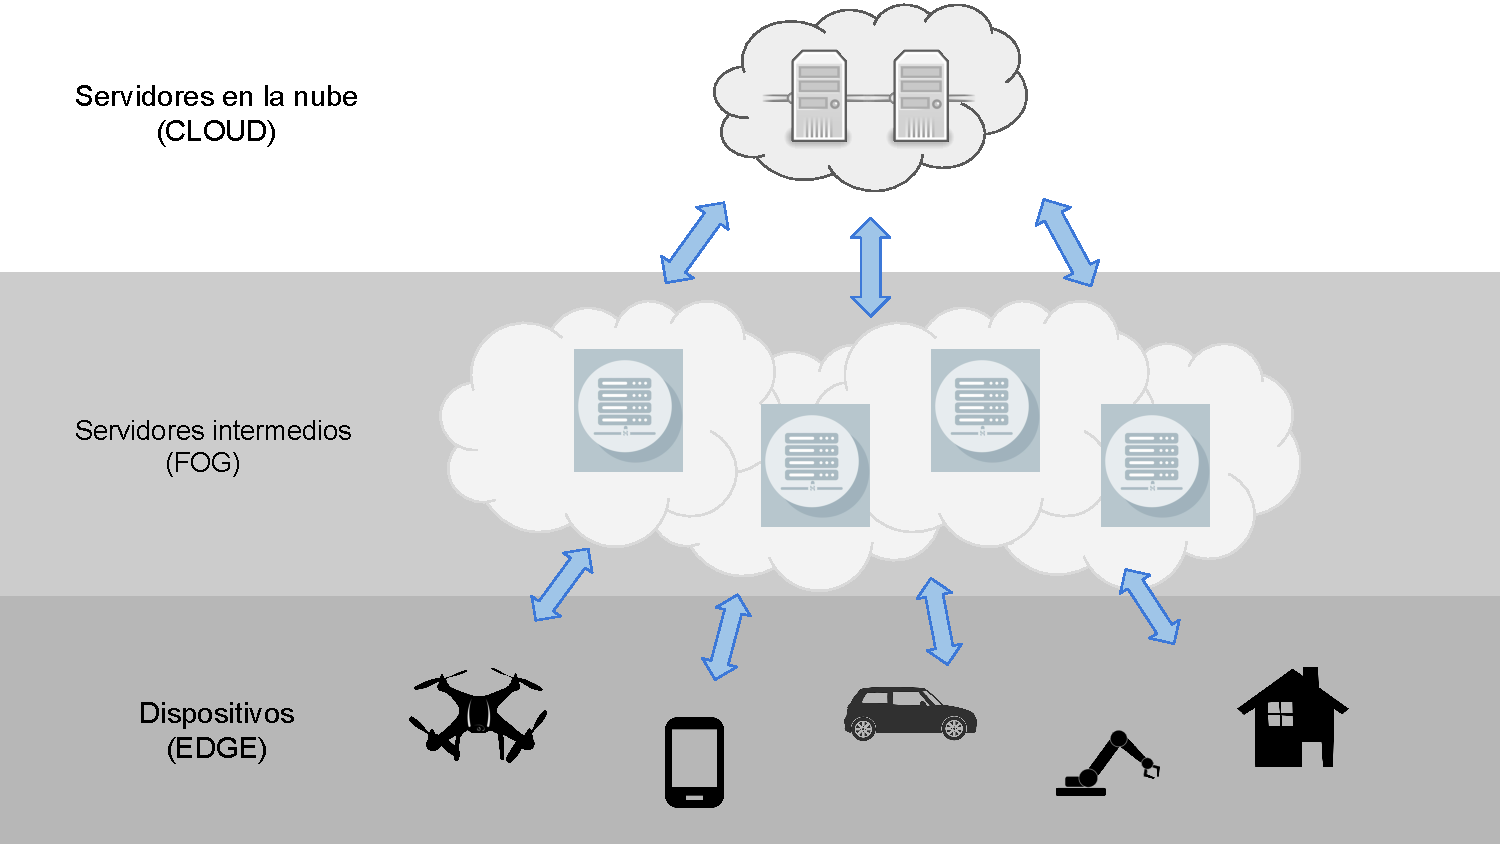
\includegraphics[width=12cm, keepaspectratio]{img/edge_computing.pdf}
  \caption{Estructura del procesamiento de los datos obtenidos por los dispositivos.}\label{fig:edge_computing}
\end{figure}

Luego, uno de los objetivos del TinyML es llevar los modelos de aprendizaje automático al extremo, es decir, a la zona de \textit{Edge computing}~\cite{Khan2019} que es el nivel más bajo donde se pueden procesar los datos, y por lo tanto, el más cercano al usuario. En la Figura~\ref{fig:edge_computing} podemos ver dónde se sitúa el \textit{Edge computing} respecto del resto de niveles donde se podrían procesar los datos. Para poder generar los modelos en esta zona se utilizan dispositivos basados en microcontroladores alimentados por batería, de forma que puedan realizar tareas de ML con capacidad de respuesta en tiempo real. Pudiendo beneficiarnos de la gran portabilidad, bajo consumo y mayor seguridad, dado que no es necesario enviar los datos a la nube, que ofrecen estas máquinas, lo que puede ser muy relevante cuando se trabaja en aplicaciones de IoT (Internet of Things)~\cite{Rose2015}. 

Los dispositivos de IoT permiten monitorear continuamente un entorno utilizando pequeños sensores. Estos dispositivos están conectados a una red por medio de la cual comparten continuamente la información obtenida. Añadir ML a un dispositivo de estas características permite detectar patrones en todos esos datos recogidos, pudiendo desarrollar una amplia gama de aplicaciones inteligentes y experiencias de usuario mejoradas. Dado que estos dispositivos son normalmente también de características reducidas, es clave el uso de técnicas de TinyML para su desarrollo.

Actualmente hay unos 250 billones de dispositivos embebidos activos en el mundo. Estos dispositivos están continuamente recogiendo grandes cantidades de datos, por lo que procesar toda esa información en la nube representa todo un desafío. TinyML podría poner solución a toda esa cantidad de datos que se están "desperdiciando" al no ser tratados ni procesados, pudiendo crear nuevas aplicaciones en diferentes tipos de industrias.

Por lo que debido a la gran importancia que están adquiriendo todos estos elementos, es importante conocer qué dispositivos cumplen las características necesarias para poder desarrollar este tipo de tareas. Es por ello que en este TFG se comprobarán las prestaciones de uno de los dispositivos de capacidades reducidas más populares del mercado, la Raspberry Pi 4B. 


%%-- Objetivos del  proyecto
%%-- Si la sección anterior ha quedado muy extensa, se puede considerar convertir
%%-- Las siguientes tres secciones en un capítulo independiente de la memoria

\section{Objetivos del proyecto}
\label{sec:objetivos}

\subsection{Objetivo general} % título de subsección (se muestra)
\label{sec:objetivo-general} % identificador de subsección (no se muestra, es para poder referenciarla)


El objetivo de este TFG es evaluar la capacidad de cómputo y eficiencia de la Raspberry Pi 4B para entrenar modelos de aprendizaje automático. Para ello se hará uso de diversos \textit{datasets} con diferentes cantidades de datos para observar su comportamiento ante diferentes entradas de datos. Y de esta forma poder concluir si este dispositivo puede ser empleado para desarrollar tareas de \textit{machine learning} e IoT o no.


\subsection{Objetivos específicos}
\label{sec:objetivos-especificos}

Para realizar este proyecto se han definido los siguientes objetivos.

    \begin{itemize}
        \item Generar diferentes modelos de aprendizaje automático utilizando la Raspberry Pi.
        \item Poner a prueba los algoritmos que entrenan los modelos, de forma que se pueda comprobar el comportamiento de la Raspberry Pi bajo diferentes condiciones de estrés.
        \item Crear y poner a prueba los mismos modelos de aprendizaje automático, pero esta vez en un dispositivo con mayor capacidad.
        \item Crear un \textit{dataset} propio para entrenar los modelos, utilizando varios sensores.
    \end{itemize}

\section{Planificación temporal}
\label{sec:planificacion-temporal}

A inicios de este curso, cuando tuve que meditar sobre qué tema quería realizar mi TFG, me di cuenta de que uno de los que más me habían gustado durante la carrera había sido \textit{machine learning}, tema que justo había comenzado a ver durante ese primer cuatrimestre. Es un tema que me interesa mucho debido a la infinidad de aplicaciones en las que creo que puede ser muy ventajoso utilizar este conocimiento, además de la capacidad que hay detrás de todos esos algoritmos para poder facilitar y mejorar la vida de las personas.

Sin embargo, no tenía del todo claro de qué forma enfocarlo. Fue entonces cuando descubrí que Katia junto con Felipe ofrecían un proyecto sobre este tema y no dudé en informarme sobre exactamente en qué estaba enfocado el trabajo. Después de contactar con Katia y proponerme varias perspectivas, me decanté por el enfoque de \textit{tiny machine learning} debido a que me llamaba la atención la posibilidad de poder observar las capacidades de la Raspberry Pi para realizar este tipo de tareas ya que, como se verá en los siguientes capítulos, es un dispositivo económico con el que se podrían ampliar la áreas donde utilizar estas técnicas.

Una vez acordado el tema lo primero que hice, a recomendación de Katia, fue informarme a cerca de cómo se podían aplicar técnicas de ML en la Raspberry Pi. En Noviembre me entregaron una caja con todo el material necesario para montar y utilizar la Raspberry Pi, con lo que el primer objetivo fue prepararla y comprobar que todo funcionase correctamente creando algoritmos simples, como por ejemplo encender y apagar un led conectado a esta máquina. Además, esta caja también traía tres sensores diferentes para utilizar con la Raspberry Pi, en concreto venia una fotoresistencia, un sensor de humedad y un sensor de temperatura, con los que realicé varias pruebas para verificar que funcionaban correctamente.

A partir de este momento y tras la primera tutoría con ambos profesores comenzó el proceso de instalación y preparación del entorno para poder implementar algoritmos de aprendizaje automático, en el que se tuvieron que superar algunas dificultades. Con el entorno instalado se procedió a implementar y realizar las pruebas oportunas.

Primero se comenzó creando los modelos de aprendizaje automático, en un principio eran tres pero más adelante se añadió un nuevo modelo de aprendizaje. Una vez que el código de los modelos estaba implementado fue momento de comenzar a realizar las pruebas para observar sus comportamientos. Estas pruebas duraron varios meses puesto que no terminaba de quedar del todo claro cómo estaba reaccionando la Raspberry Pi ante las diferentes pruebas, es por ello que durante este periodo se utilizaron diferentes \textit{datasets} para seguir haciendo más pruebas y entender lo que estaba sucediendo.

Una vez esclarecidas las dudas se trató de ir más allá haciendo que la Raspberry Pi generase su propio \textit{dataset} y entrenase con él. Este fue el último paso antes de centrarme completamente en la redacción de la memoria. A lo largo de los meses, además de seguir avanzando con la investigación, también trataba de ir redactando poco a poco la memoria.

A pesar de que el desarrollo de este trabajo comenzó en Noviembre no fue hasta finalizar el primer cuatrimestre cuando le empecé a dedicar como mínimo hora y media o dos horas todos los días, salvo algunas excepciones. Siendo los fines de semana cuando le dedicaba aún más tiempo por no tener ninguna otra ocupación. En la Figura~\ref{fig:diagrama_gantt} se puede observar un diagrama de Gantt donde se puede visualizar mejor el desarrollo y duración de cada una de las etapas del proyecto.


\begin{figure}[htb]
  \centering
  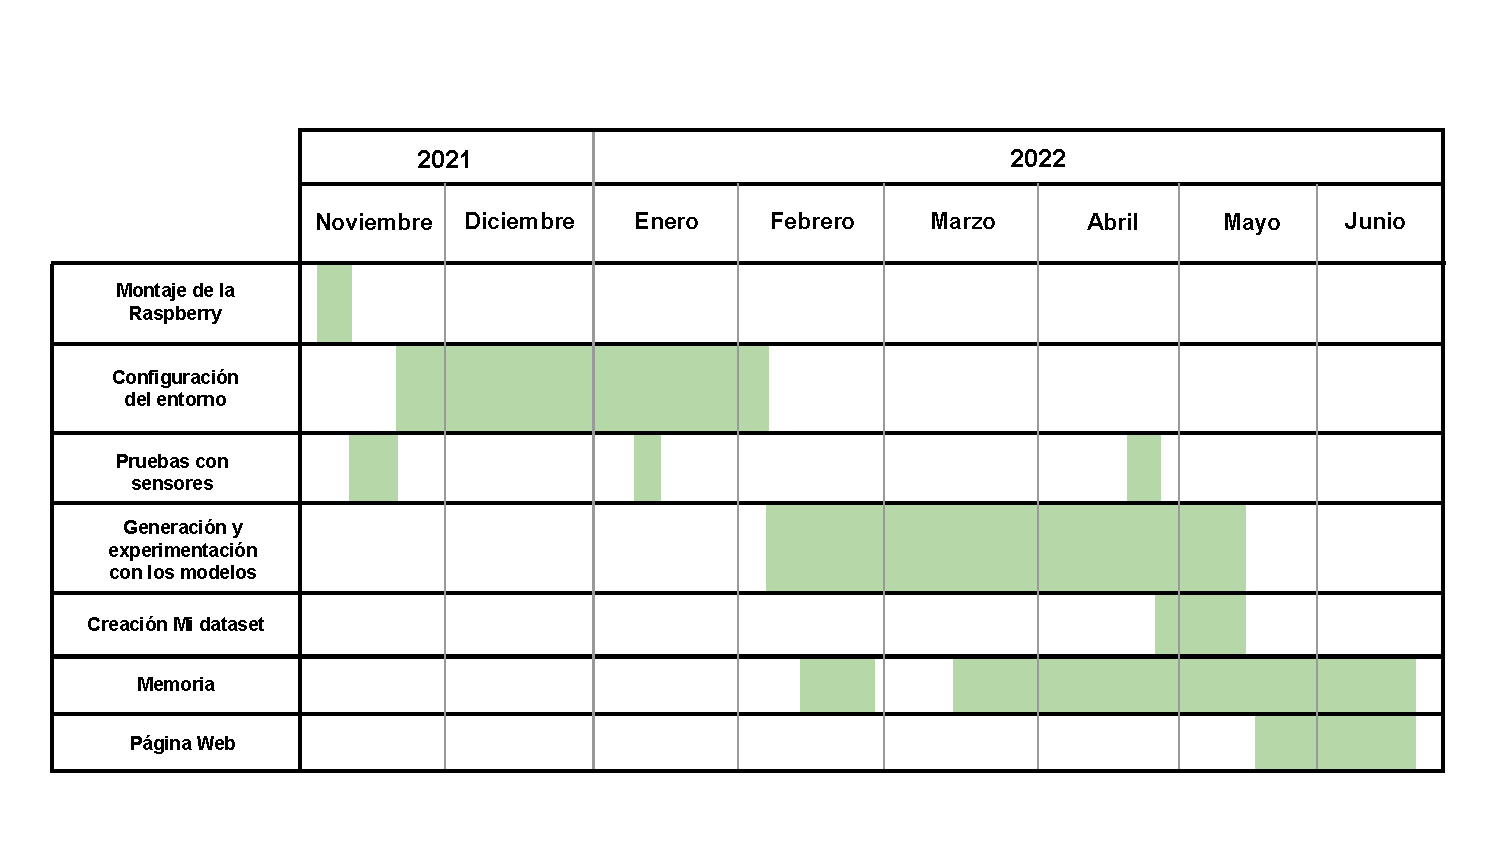
\includegraphics[width=17cm, keepaspectratio]{img/diagrama_GANTT.pdf}
  \caption{Diagrama de Gantt donde se representa la planificación temporal llevada a cabo en este proyecto.}\label{fig:diagrama_gantt}
\end{figure}

\section{Estructura de la memoria}
\label{sec:estructura}

Al inicio de esta memoria se puede leer un resumen de la misma que indica en qué consiste el trabajo desarrollado. A continuación se sitúan los agradecimientos además de tres índices, el general, el de las figuras y el índice de fragmentos de código. Por último, se encuentran los 6 capítulos en los que se divide la memoria.

\begin{itemize}

    \item \textbf{Capítulo 1: Introducción.} En este capítulo se realiza una descripción general de en qué consiste el proyecto. Especificando los objetivos del proyecto, la planificación del mismo y cual es la estructura de la memoria.
    \item \textbf{Capítulo~\ref{chap:tecnologias}: Estado del arte.} Aquí se explican todas las tecnologías utilizadas en el desarrollo del trabajo.
    \item \textbf{Capítulo~\ref{chap:diseño}: Diseño e implementación.} Se describe de forma detallada la arquitectura general del proyecto, la configuración del entorno para llevar a cabo la investigación, así como el código empleado para generar los modelos de aprendizaje y los \textit{datasets} utilizados para entrenarlos.
    \item \textbf{Capítulo~\ref{chap:experimentos}: Experimentos y validación}. Por una parte se explica en que consisten las pruebas realizadas tanto en la Raspberry Pi como en el portátil, además de explicar cómo y qué código se utiliza para ejecutarlas. Por otra parte se exponen y explican los resultados obtenidos para cada uno de los modelos generados por los diferentes \textit{datasets} en cada una de las pruebas.
    \item \textbf{Capítulo~\ref{chap:conclusiones}: Conclusiones}. Se exponen las conclusiones obtenidas gracias a esta investigación. Además de detallar posibles proyectos derivados de este proyecto.
    \item \textbf{Capítulo~\ref{chap:anexo}: Anexo.} Se detallan algunas características y especificaciones para la instalación correcta del entorno.
\end{itemize}

\section{Enlaces de interés}
\label{sec:enlaces_interes}

En la siguiente URL: se puede encontrar un resumen general en inglés de todo aplicado y desarrollado en este trabajo. Además desde ese enlace también se puede acceder al repositorio de \textit{GitHub} que contiene este proyecto así como al propio pdf de la memoria.

\cleardoublepage

%%%%%%%%%%%%%%%%%%%%%%%%%%%%%%%%%%%%%%%%%%%%%%%%%%%%%%%%%%%%%%%%%%%%%%%%%%%%%%%%
%%%%%%%%%%%%%%%%%%%%%%%%%%%%%%%%%%%%%%%%%%%%%%%%%%%%%%%%%%%%%%%%%%%%%%%%%%%%%%%%
% ESTADO DEL ARTE %
%%%%%%%%%%%%%%%%%%%%%%%%%%%%%%%%%%%%%%%%%%%%%%%%%%%%%%%%%%%%%%%%%%%%%%%%%%%%%%%%

\chapter{Estado del arte}               %% a.k.a "Tecnologías utilizadas"
\label{chap:tecnologias}

En este capítulo se describen todas las tecnologías utilizadas en el desarrollo de este proyecto.

\section{Machine learning}
\label{sec:machine_learning}

Para saber si la Raspberry Pi es un dispositivo lo suficientemente potente para realizar tareas de \textit{machine learning} primero debemos tener claros estos conceptos para poder entender el proyecto.

 El \textit{machine learning} o aprendizaje automático, es una disciplina del campo de la Inteligencia Artificial que se centra en la construcción de programas software y sistemas de información capaces de mejorar la resolución de una tarea conforme ganan experiencia. Para aprender utilizan algoritmos que permiten a los ordenadores identificar los patrones que existen en grandes cantidades de datos y utilizar estos patrones para poder elaborar predicciones del futuro. 
 
 Los datos que se proporcionan al algoritmo normalmente son ficheros con varias filas y columnas. Cada fila representa un ejemplo de datos que se pasa al modelo para entrenar. Mientras que si poseen varias columnas significa que hay varios valores que definen un ejemplo, se dice que estas columnas son las características del \textit{dataset}. 
 
 Un ejemplo de lo que contiene un \textit{dataset} es la tabla~\ref{tab:my_dataSet}, donde se proporciona información sobre cuando un niño va a jugar a la pelota o no. En este caso tendríamos tres características (previsión, temperatura y amigos), la columna "Jugar" es la decisión que toma el niño ante los valores de esas características. Por lo tanto, cada fila define una situación diferente, es decir, es un ejemplo de lo que puede suceder.
 
 \begin{table}[htb]
     \centering
     \begin{tabular}{ c  c  c  c }
          \toprule
          Previsión & Temperatura & Amigos & Jugar\\
          \midrule
           Soleado &  25 ºC & 2 & Si \\
           Lluvioso &  12 ºC & 0 & No\\
           Nublado &  18 ºC & 4 & Si\\
           \bottomrule
     \end{tabular}
     \caption{Ejemplo de un \textit{dataset}}
     \label{tab:my_dataSet}
 \end{table}
 
 Los algoritmos de ML se pueden encuadrar, entre otras, en tres categorías~\cite{James2021}: 

\begin{itemize}
    \item \textbf{Aprendizaje supervisado}. En este tipo de aprendizaje se le proporciona al algoritmo un conjunto de datos de entrada con su salida correspondiente. De esta forma el programa puede "aprender" la relación que existe entre la salida y el conjunto de entradas. Dependiendo del tipo de salida podremos encontrar dos clases de modelos: modelos de regresión o de clasificación.
    
    Si la salida es un valor numérico continuo, estaríamos ante un problema de regresión en el que se busca obtener el modelo que mejor se ajusta a los datos de entrada para poder predecir otros valores. Si, en cambio, la salida es una etiqueta de clase, es decir un valor discreto, se correspondería a un problema de clasificación, en los que se busca estimar a qué clase pertenecen los datos de entrada. 
    
    Un ejemplo de este último tipo se puede ver en la Figura~\ref{fig:a_supervisado}, donde cada una de las formas serían las entradas y las etiquetas de: triángulo, cuadrado o círculo serían la salidas. Cada dato de entrada tiene asignada una de estas etiquetas. Todo esto formaría lo que se denomina \textit{dataset} que es el conjunto de datos que se pasan al modelo para entrenar y poder encontrar esas relaciones entre entradas y salidas. En este caso cuando al modelo se le pregunte a qué clase pertenece una figura (del mismo tipo que ha visto durante el entrenamiento), si es lo suficientemente robusto, debería de ser capaz de identificarlo como un cuadrado.
    
    \begin{figure}[htb]
      \centering
      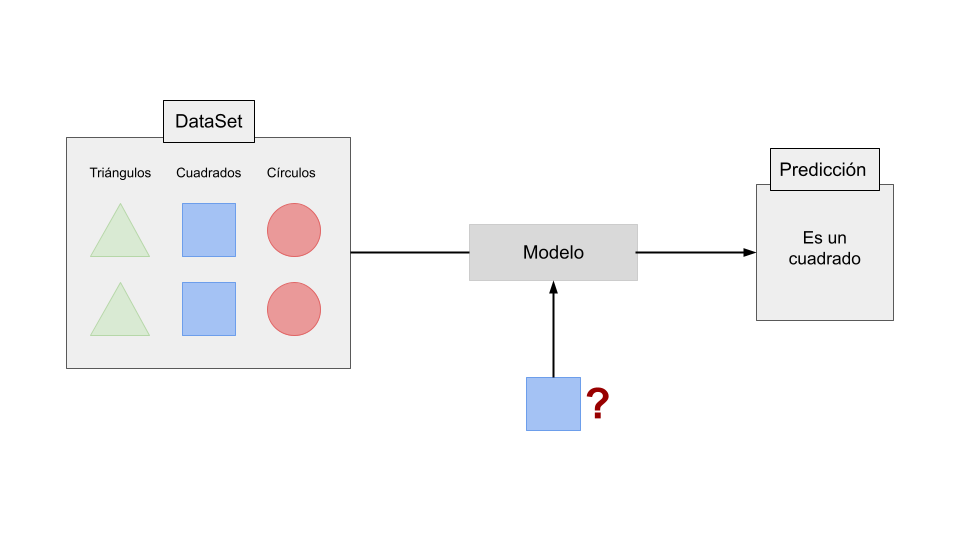
\includegraphics[width=12cm, keepaspectratio]{img/a_supervisado.png}
      \caption{Estructura aprendizaje supervisado para clasificación.}\label{fig:a_supervisado}
    \end{figure}
    
    Existen multitud de modelos de \textit{machine learning} que sirven para resolver problemas mediante aprendizaje supervisado, como por ejemplo algoritmos de Regresión Logística, Árboles de Decisión, Máquinas de Vector Soporte...
    
    \item \textbf{Aprendizaje no supervisado}. Al algoritmo de aprendizaje se le proporciona únicamente el conjunto de datos de entrada, sin ningún tipo de dato de salida. El objetivo es que el método de aprendizaje utilizado detecte posibles patrones de interés en el conjunto de datos de entrada. 
    
    \begin{figure}[htb]
      \centering
      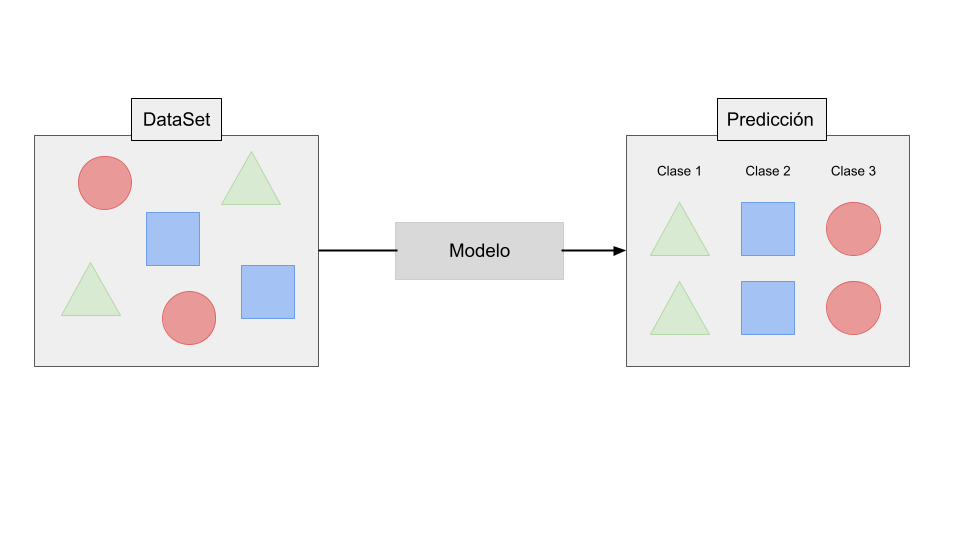
\includegraphics[width=12cm, keepaspectratio]{img/a_no_supervisado.png}
      \caption{Estructura aprendizaje no supervisado para segmentación.}\label{fig:a_no_supervisado}
    \end{figure}
    
    Hay principalmente dos tipos de tareas que estos algoritmos tratan de realizar. Una de ellas es el \textit{clustering} (o segmentación), que sirve para encontrar diferentes grupos dentro de los datos de entrada. En la Figura~\ref{fig:a_no_supervisado} se muestra un ejemplo esquemático de la ejecución de un problema de este estilo, donde una vez más las entradas serían cada una de las formas pero en esta ocasión no están etiquetadas como veíamos en la Figura~\ref{fig:a_supervisado}. El modelo, viendo las características de cada uno de los datos, los agrupará en diferentes clases.
    
    La otra misión que puede tener este tipo de aprendizaje es reducir la dimensionalidad de los datos, es decir, reducir el número de características del conjunto de datos de entrada asumiendo que muchas de ellas son redundantes y por lo tanto no aportan información nueva.
    
    Al igual que en aprendizaje supervisado existen varios algoritmos que buscan resolver estas tareas, como por ejemplo el método \textit{k}-NN, \textit{k-means}...
    
    \item \textbf{Aprendizaje por refuerzo}. El algoritmo aprende a desarrollar la tarea que se le asigna en base a un esquema de recompensas y penalizaciones ante las decisiones que toma el programa en cada una de las iteraciones. Luego, por cada acción que realice el modelo recibirá una recompensa o una penalización, de esta forma podrá tener conocimiento de si ha tomado una buena o mala decisión. El objetivo es que llegue a realizar la tarea encomendada consiguiendo la mayor recompensa posible.
\end{itemize}

Gracias a que todos estos algoritmos pueden estar aprendiendo constantemente de nuevos datos consiguen ir perfeccionando su comportamiento, lo que hace que las técnicas de ML sean cada vez más importantes debido a la multitud de aplicaciones que se le pueden dar dentro de la robótica, los vehículos autónomos, diagnósticos médicos, markenting....

\subsection{Tiny machine learning}
\label{subsec:tinyML}

\textit{Tiny machine learning}\cite{Warden2020,TinyML}, cuyo origen se encuentra en el \textit{machine learning}, es la unión del aprendizaje automático con los dispositivos IoT. Es decir, consigue que dispositivos con menor capacidad de cómputo sean capaces de ejecutar algoritmos de ML. Es una disciplina emergente con la que se amplían la posibilidades de utilizar los algoritmos de m\textit{achine learning} en un mayor número de máquinas.

Tradicionalmente, los dispositivos IoT tenían que enviar los datos recogidos a la nube para procesarlos y poder generar el modelo de aprendizaje automático con la información proporcionada. Con TinyML conseguimos que estas tareas las realice el propio dispositivo IoT, sin necesidad de enviar nada a la nube. Gracias a esto adquirimos: 

\begin{itemize}
    \item Mayor privacidad y seguridad. Los datos no tienen que estar enviándose a ningún sitio, evitando que puedan ser interceptados y usados de forma maliciosa.
    \item Menor latencia. El tiempo de respuesta será menor puesto que todo el procesamiento se hace en el mismo dispositivo que tiene que responder. Esto es mucho más eficiente que tener que enviar la información y esperar hasta que otra máquina la procese y envíe la respuesta.
    \item Mayor eficiencia energética. Puesto que estar continuamente transmitiendo información (a través de cables o de forma inalámbrica)consume mucha energía.
\end{itemize}

\section{Modelos de Aprendizaje Automático}
\label{sec:modelos_aautomatico}

Aunque existen muchos algoritmos para generar modelos de aprendizaje automático, en este proyecto vamos a utilizar concretamente cuatro: Regresión Logística (RL), Máquinas de Vector Soporte (SVM), Gradient Boosting (GB) y Random Forest (RF). Para ello se utilizará la librería de \texttt{scikit-learn}, que veremos más adelante.

\subsection{Regresión Logística}
\label{subsec:regresion_logistica}

Modelo de aprendizaje supervisado que realiza tareas de clasificación binaria, es decir solo existen dos posibles clases. Esta técnica busca una función acotada (normalmente entre 0 y 1) que divida los datos de ambas clases de forma bien diferenciada. Normalmente dicha función se denomina como Logística o sigmoide y se define de la siguiente forma~\cite{Watt2020}:

\begin{equation}
    h_w(x^{(i)}) = \frac{1}{1 + e^{\sum_{j=0}^{d} w_j x_j^{(i)} }}
\end{equation}

Esta expresión devolverá un valor entre cero y uno. Según lo próximo que este el valor a cero o uno pertenecerá a una clase u otra. 

Los parámetros representados por $w$ son los pesos, unos valores numéricos que utiliza la función para realizar la predicción. Cada peso está multiplicando a una característica, representada mediante $x_j$. Por tanto, para conocer a qué clase pertenece el ejemplo $x^{(i)}$ habrá que aplicar la fórmula anterior, por lo que se tendrá que realizar el sumatorio de todos los pesos multiplicados por sus respectivas características (desde la cero hasta la d-ésima). 

Durante la fase de entrenamiento el modelo ajusta los pesos mediante un método de optimización, a fin de que las predicciones que se realicen mediante ellos tengan el mínimo error posible. Para obtener los valores óptimos de los pesos se utiliza el método de descenso por gradiente, mediante el cual se irán actualizando los valores de los pesos conforme vaya entrenando con más ejemplos. La función de descenso por gradiente se define en la ecuación~\ref{eq:desc_gradiente}.

\begin{equation}
    w_j = w_j - \alpha \frac{1}{n} \sum_{i= 1}^{n} (h_w(x^{(i)}) - y^{(i)}) x_j^{(i)}
    \label{eq:desc_gradiente}
\end{equation}

Para calcular los pesos se utiliza el error que existe entre la salida predicha con los pesos estimados hasta ahora ($h_w(x^{(i)})$) y el valor real, es decir, la salida que verdaderamente corresponde a ese ejemplo ($y^{(i)}$). También es necesario definir el valor del ratio de aprendizaje ($\alpha$), si se le da un valor muy elevado puede llegar a no converger el modelo en ninguna solución. Esto se realiza para todos los valores de $j$, desde $j= 0$ hasta $j= d$, que es el número total de características.

Se dará por finalizada la fase de aprendizaje cuando se consiga que los valores de los pesos minimicen una función de coste:

\begin{equation}
    J(w) = \frac{1}{2} \sum_{i= 1}^{n} {(h_w(x^{(i)}) - y^{(i)})}^2 
\end{equation}


\subsection{Máquinas de Vector Soporte}
\label{subsec:maquinas_vector_soporte}

Modelo de aprendizaje supervisado utilizado para resolver tareas de clasificación binaria, aunque existen Máquinas de Vector Soporte para resolver problemas de regresión o de clasificación multiclase. Se basa en la generación de un hiperplano que separe de forma óptima los puntos de una clase respecto de otra~\cite{Duda2001}. Es decir, que exista la máxima distancia entre el hiperplano y los puntos más cercanos a este, los puntos más cercanos al hiperplano de separación se denominan como vectores soporte. Así pues, el hiperplano óptimo pasará justo por el medio de los vectores soporte de ambas clases.

\begin{figure}[htb]
  \centering
  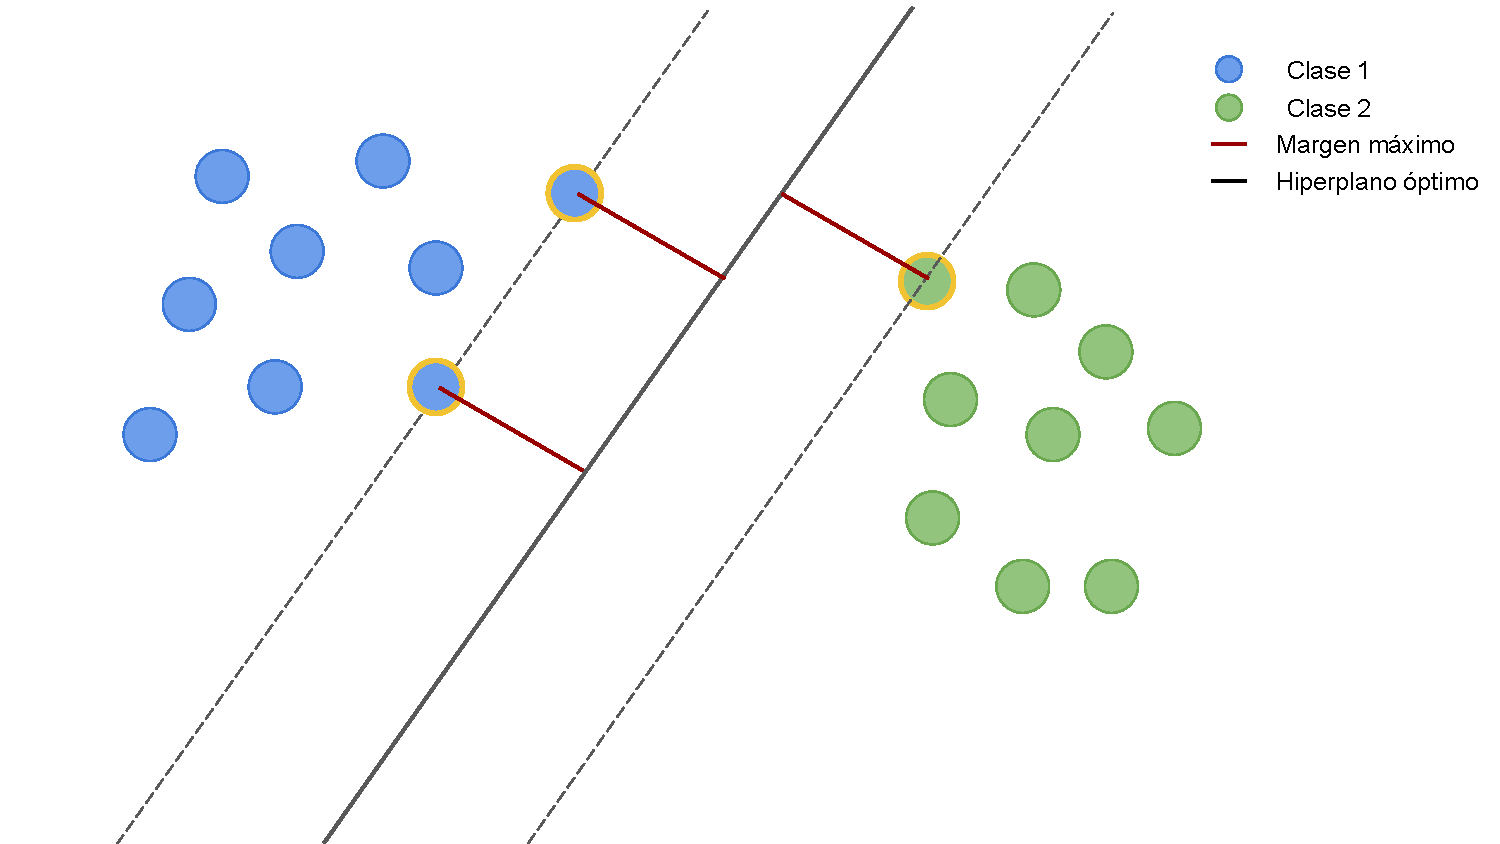
\includegraphics[width=11cm, keepaspectratio]{img/explicacion_SVM.pdf}
  \caption{Ejemplo clasificación con Máquinas de Vector Soporte}\label{fig:explicacion_svm}
\end{figure}

En la Figura~\ref{fig:explicacion_svm} se puede ver un ejemplo de separación óptima entre ambas clases, siendo los círculos rodeados en amarillo los vectores soporte. Todos tienen la máxima distancia posible con el hiperplano generado, que es capaz de separar perfectamente ambas clases. El hiperplano de separación se puede definir como una función lineal:

\begin{equation}
    h(x) = \sum_{i= 0}^{n} w_i x_i
\end{equation}

En esta ocasión también se utilizan unos pesos ($w$) para encontrar dicho hiperplano.

Sin embargo, hay veces que puede llegar a ser imposible hallar un hiperplano que divida correctamente las clases. Ante estos casos la resolución del problema se encuentra en aumentar la dimensionalidad de los datos para comprobar si en esa nueva dimensión existe un hiperplano capaz de separarlos adecuadamente. Otra solución es relajar las condiciones de búsqueda de hiperplano de separación, de forma que se tolere que algunos puntos caigan en el lado incorrecto (\textit{hard-margin} vs. \textit{soft-margin}).


\subsection{Gradient Boosting}
\label{subsec:gradient_boosting}

Técnica de aprendizaje supervisado que se utiliza tanto para problemas de regresión como de clasificación. Se basa en la combinación de modelos predictivos débiles, normalmente árboles de decisión, para crear un modelo predictivo fuerte~\cite{James2021}. Los árboles de decisión son uno de los algoritmos más utilizados para la toma de decisiones debido a su sencilla implementación y fácil interpretación. Dado un conjunto de datos, se crean diagramas lógicos que sirven para representar una serie de condiciones sucesivas para resolver un problema. Por ejemplo, en la Figura~\ref{fig:ejemplo_adecision} hay representado un árbol de decisión que sirve para poder saber si podemos salir a la calle a correr, dependiendo de ciertas condiciones se hará una cosa u otra. 

\begin{figure}[htb]
  \centering
  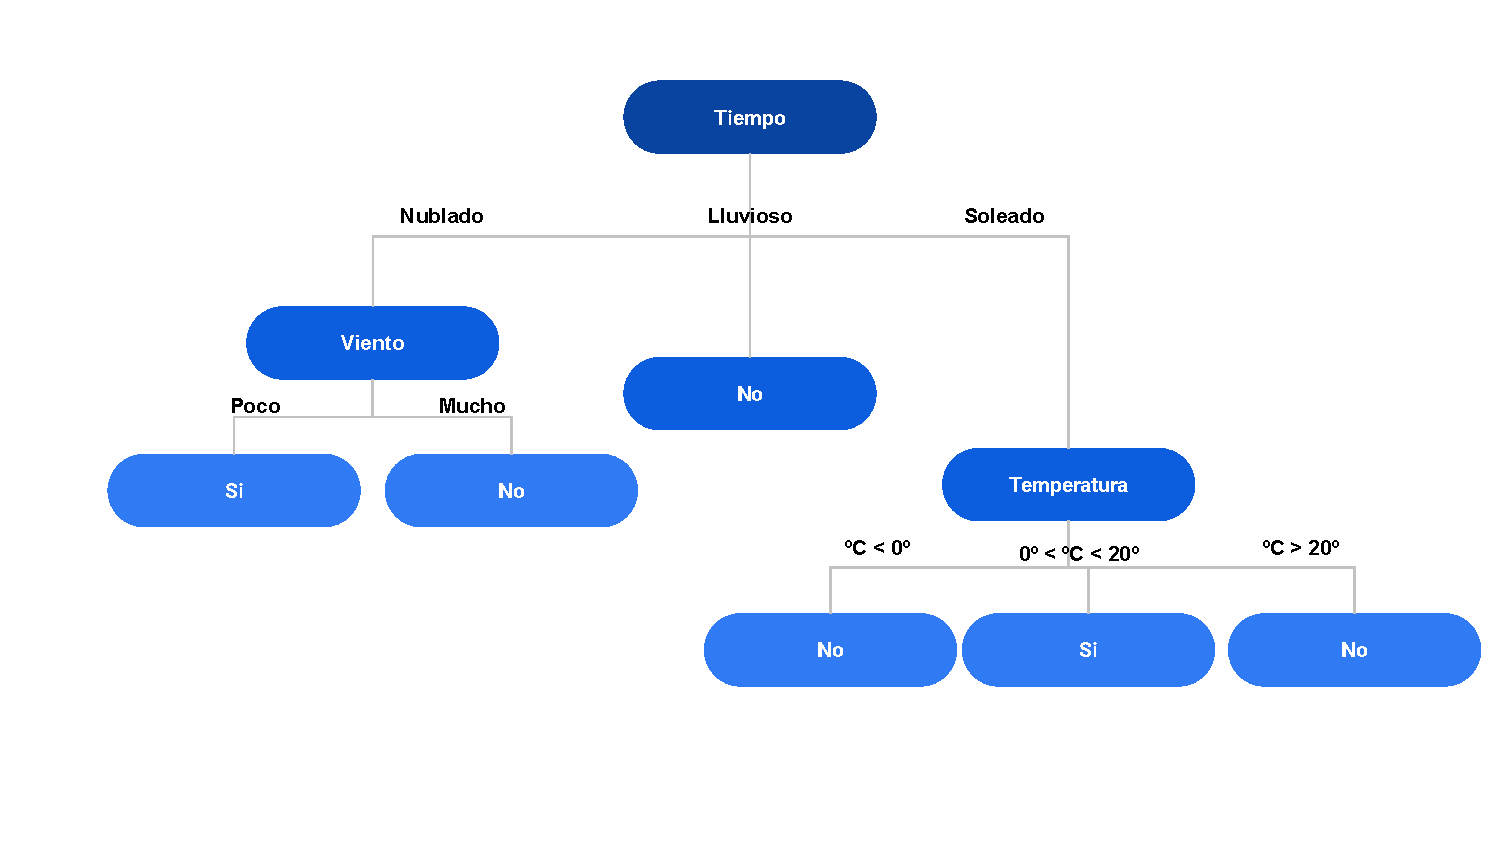
\includegraphics[width=16cm, keepaspectratio]{img/ejemplo_adecision.pdf}
  \caption{Ejemplo árbol de decisión.}\label{fig:ejemplo_adecision}
\end{figure}

En Gradient Boosting (GB) se generan árboles de decisión de forma secuencial, haciendo que cada árbol corrija los errores del árbol anterior. De forma general suelen ser árboles de un máximo de tres niveles de profundidad.

\subsection{Random Forest}
\label{subsec:random_forest}

Random Forest se puede usar tanto en problemas de clasificación como de regresión. Este modelo utiliza un conjunto de árboles de decisión, que se generan de forma paralela, para realizar las predicciones. Cada uno de los árboles de decisión se entrena con un subconjunto aleatorio de los datos de entrenamiento~\cite{James2021}. 

Cuando se quiera, por ejemplo, estimar la clase a la que pertenece un dato cada uno de los árboles "votará" por la clase a la que cree que el dato pertenece. La clase con mayoría de votos es la predicción final del modelo. Por lo tanto, aumentando el número de árboles de decisión se aumenta la precisión del modelo. Con lo que se consigue construir un modelo robusto a partir de varios modelos que no tienen por qué ser tan robustos.

\begin{figure}[htb]
  \centering
  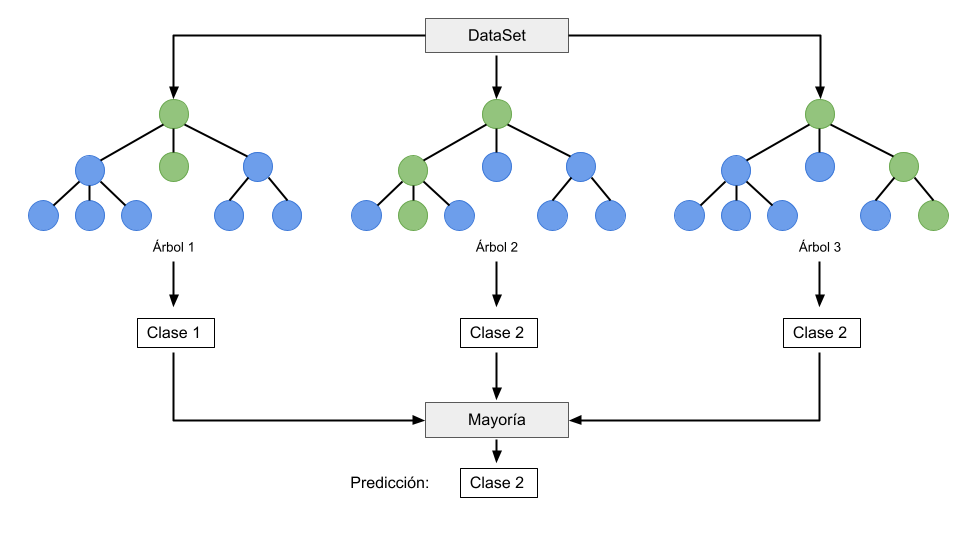
\includegraphics[width=14cm, keepaspectratio]{img/ejemplo_randomForest.png}
  \caption{Ejemplo Random Forest.}\label{fig:ejemplo_rforest}
\end{figure}

En la Figura~\ref{fig:ejemplo_rforest} podemos ver un ejemplo de Random Forest. Con el \textit{dataset} que se le pasa generará, en este caso, tres árboles de decisión a partir de subconjuntos aleatorios del \textit{dataset} original. Cuando se pretenda clasificar un nuevo dato cada árbol le asignará una clase a ese dato según lo que haya decidido. La clase que más se repite en este ejemplo es la 2, por lo tanto esa será la clase a la que pertenezca el dato.

\section{Internet of Things (IoT)}
\label{sec:IoT}

Uno de los campos en los que son de gran importancia las técnicas de aprendizaje automático es en los proyectos de IoT (Internet of Things)~\cite{Rose2015}. El Internet de las Cosas (o Internet of Things) es la interconexión de sensores y dispositivos, como por ejemplo pueden ser los electrodomésticos, termostatos, coches, ropa... Todos ellos se comunican a través de una red por medio de la cual pueden interaccionar entre ellos y compartir datos sin necesidad de que un humano intervenga, esta red puede ser por cable, WiFi, Bluetooth etc. 

Los dispositivos conectados generan una gran cantidad de datos que llegan a una plataforma IoT que recolecta, procesa y analiza dichos datos. Utilizando \textit{machine learning} se puede generar, por medio de todos estos datos recopilados, nuevos modelos de aprendizaje automático cuyas predicciones se pueden usar para poder actuar sobre el entorno. Las posibles aplicaciones que ofrece esto son prácticamente infinitas, algunos ejemplos pueden ser:

\begin{itemize}
    \item \textit{Smart Homes}. Permite que se puedan controlar varios de los dispositivos que hay comúnmente en los hogares haciendo que, por ejemplo, esté listo todo lo que necesite el usuario para cuando llegue a casa.
    \item Telemedicina. Por medio de dispositivos que lleve puesto el paciente se puede tener un control sobre su estado de salud e incluso hacer diagnósticos anticipados.
    \item Vehículos autónomos. Los vehículos puedan estar conectados a la red de tráfico en tiempo real para poder evitar accidentes.
\end{itemize}

\section{Dispositivo con capacidad de cómputo limitada: Raspberry Pi 4 Modelo B}
\label{sec:dispositivo_hardware}

Raspberry Pi\footnote{\url{https://www.raspberrypi.org/}} es un ordenador de bajo coste y tamaño reducido desarrollado por Raspberry Pi Foundation. Este dispositivo se puede emplear en  multitud de aplicaciones pero su principal objetivo es hacer accesible la informática a todos los usuarios. A parte de poder realizar todas las tareas que se esperan de un ordenador, también puede interactuar con el entorno a través de sensores conectados a sus pines GPIO.

\begin{figure}[htb]
  \centering
  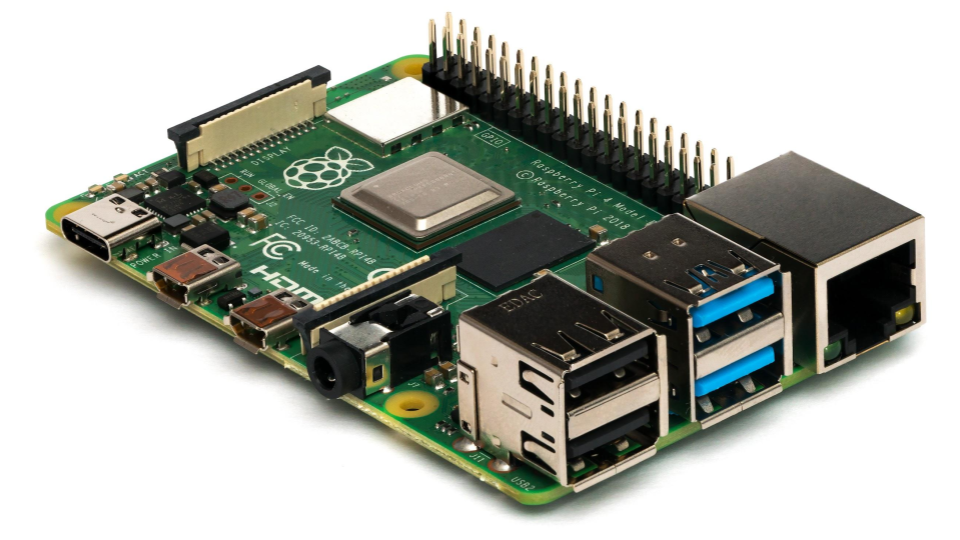
\includegraphics[width=10cm, keepaspectratio]{img/real_raspberry.png}
  \caption{Raspberry Pi 4 Modelo B.}\label{fig:raspberry_pi}
\end{figure}

El sistema operativo que ofrece es Raspbian Pi OS, una versión adaptada de Debian. Sin embargo, permite poder utilizar otros sistemas.

Desde su primer lanzamiento se han ido desarrollando y comercializando nuevos modelos. En este proyecto se utilizará la última versión de estos dispositivos denominado como Raspberry Pi 4 Modelo B con 4GB de RAM, en la Figura~\ref{fig:raspberry_pi} se puede ver como es este dispositivo. Dicho modelo posee un total de 40 pines GPIO, 2 puertos micro HDMI y 4 puertos USB. Puede realizar conexiones inalámbricas ya que tiene Bluetooth 5.0 y Wi-Fi, aunque también puede utilizar Ethernet. Por último, la alimentación viene dada por un cable USB de tipo C con el que puede alcanzar un total de 1.2 A.

Posee un procesador ARM Cortex-A72 que soporta SIMD avanzado, un tipo de unidad de ejecución que se utiliza para ejecutar la misma instrucción sobre varios datos al mismo tiempo, consiguiendo paralelismo a nivel de datos. En total, la Raspberry Pi tiene cuatro cores físicos y cuatro lógicos. 

Otro detalle destacable de la Raspberry Pi para el desarrollo de este trabajo es que posee una arquitectura SMP (Symmetric Multi-Processing), un tipo de arquitectura de computador en el que las unidades de procesamiento comparten una única memoria central, lo que permite que cualquier procesador trabaje en cualquier tarea sin importar su localización en memoria. 

Actualmente es uno de los dispositivos más populares ya que brinda un sinfín de posibilidades a pesar de su pequeño tamaño. Específicamente dentro del campo de aprendizaje automático e IoT, se podrían desarrollar multitud de aplicaciones gracias a la interacción que tiene con el entorno por medio de los sensores y actuadores que se le pueden conectar. Por ello, en este trabajo de investigación se busca examinar el rendimiento de este pequeño ordenador y comprobar hasta donde se podría llegar con él, dentro del campo del aprendizaje automático~\cite{Garcia-Martin2019}. 


\section{Sensores}
\label{sec:sensores}

En este proyecto también se utilizaron sensores para tomar medidas del entorno y generar nuestro propio \textit{dataset} con el que entrenar los modelos de aprendizaje automático. En concreto se utilizaron dos: una fotoresistencia (LDR) y un sensor BME280, a continuación se darán más detalles de ambos sensores.

\subsection{Fotoresistencia}
\label{subsec:fotoresistencia}

Esta resistencia, también denominada como LDR por sus siglas en inglés Light Dependent Resistor, varía su resistencia dependiendo de la cantidad de luz que incida sobre su superficie. Funciona gracias al principio de la fotoconductividad que es un fenómeno óptico en el que la conductividad del material aumenta cuando la luz es absorbida. Así pues, cuando la luz cae sobre la resistencia los electrones son excitados lo que provoca que empiece a fluir cada vez más corriente a través del dispositivo, por lo que la resistencia del dispositivo disminuye. Por lo tanto, cuando el LDR recibe luz, su resistencia será más baja y cuando esté a oscuras la resistencia será más alta. La resistencia del LDR está en torno a los $5 k\Omega$

Para que la Raspberry Pi pueda obtener el valor que devuelve este sensor es necesario utilizar un conversor. En este caso utilizaremos el HW-103, que al conectarlo a la Raspberry Pi y a el sensor podremos conseguir una señal digital. Cuando a la Raspberry Pi le llegue un cero significará que hay luz mientras que si lee un uno es que no hay luz.

\subsection{BME280}
\label{subsec:bme280}

El sensor BME280\footnote{\url{https://www.bosch-sensortec.com/products/environmental-sensors/humidity-sensors-bme280/}}, desarrollado por Bosch, es un sensor creado especialmente para aplicaciones móviles y prendas de vestir, donde el tamaño y el bajo consumo de energía son elementos claves. Integra en un mismo dispositivo tres sensores diferentes que proveen medidas de alta precisión. Los tres sensores que posee son: uno de temperatura, otro de presión atmosférica y por último, uno de humedad relativa. 

El rango de la temperatura va desde los $-40\, \mbox{ºC}$ hasta los $85\, \mbox{ºC}$, con una precisión de $\pm 0.5\, \mbox{ºC}$. El sensor de presión tiene un rango de entre $300 hPa$ y $1100 hPa$. Por último el rango de la humedad relativa va desde el 0 hasta el 100\%.

La comunicación con este sensor es muy sencilla ya que puede usar tanto I2C o SPI. Tiene una tensión de funcionamiento de $3.3V$. Y a pesar de que integra tres sensores diferentes su tamaño es pequeño, concretamente de $19x18 mm$.

Este tipo de sensores se utilizan en aplicaciones como: monitorización del clima, automatización del hogar, sistemas de autopiloto para drones...Y se ajusta muy bien a las necesidades de este proyecto ya que tiene un consumo y tamaño muy pequeño, por lo que sería factible implementar una aplicación de IoT con él.


\section{Sistema Operativo: Ubuntu 21.10} 
\label{sec:sistema_operativo}

El sistema operativo Ubuntu\footnote{\url{https://ubuntu.com/}} es una distribución de código abierto basada en Debian, está compuesto de software normalmente distribuido bajo una licencia libre o de código abierto. La empresa responsable de su creación y mantenimiento es Canonical, una empresa de programación de ordenadores con base en Reino Unido fundada por el empresario Mark Shuttleworth.

La primera versión de Ubuntu fue la 4.10 lanzada el 20 de Octubre de 2004. A partir de la versión 13.4 las versiones estables sin soporte a largo plazo se liberan cada seis meses, y Canonical proporciona soporte técnico y actualizaciones de seguridad durante 9 meses. Las versiones LTS (Long Term Support) ofrecen un soporte técnico durante 5 años a partir de la fecha de lanzamiento.

La última versión fue lanzada el 14 de Octubre de 2021, que es la versión Ubuntu 21.10. Utiliza el kernel 5.13, con cambios y mejoras para componentes que daban problemas. También tiene un nuevo instalador, escrito desde cero en Flutter, que facilita la instalación del sistema operativo. Una de las novedades más importantes es que actualiza su escritorio a GNOME 40. 

Es una versión es específica para el procesador ARM, compilada con 64-bits y será la versión que se utilizará en la Raspberry Pi, a pesar de que no sea lo más común utilizarlo en estos dispositivos. También esta será la versión del sistema operativo del portátil.

\subsection{Gestor de paquetes: Miniforge}
\label{subsec:gestor_de_paquetes}

%%-- El comando \gls{} permite incluir términos en el glosario, para luego reunirlos todos
%%-- en una tabla al comienzo o al final del documento, junto con sus definiciones.

Miniforge\cite{Miniforge} es un instalador mínimo de Conda especifico de conda-forge, que permite instalar el manejador de paquetes Conda con una serie de configuraciones predefinidas. Es muy similar a un instalador de Miniconda.

Miniconda es un sistema de gestión de paquetes y entornos virtuales. Mediante él se instala una pequeña versión de arranque de Anaconda que incluye solo conda, Python, los paquetes de los que dependen y otros pocos paquetes útiles como pueden ser pip, zlib...

Ofrece casi lo mismo que Anaconda pero es mucho más ligero, lo que lo hace idóneo para poder desarrollar el proyecto en el dispositivo utilizado. Además, facilita la replicación de un entorno concreto ya que permite tener un mayor control y orden sobre los paquetes que se instalan. 

\section{Lenguaje de programación: Python}
\label{sec:lenguaje_de_programación}

Python\footnote{\url{https://www.python.org/}} es un lenguaje de programación que nace a principios de los años 90 gracias al informático holandés Guido Van Rossum. Su objetivo era crear un lenguaje de programación que fuera fácil de aprender, escribir y entender.

Es un lenguaje de alto nivel (sencillo de leer y escribir debido a su similitud con el lenguaje humano), interactivo, interpretado y orientado a objetos. Al ser interpretado permite poder ejecutarlo sin necesidad de compilarlo previamente, reduciendo el tiempo entre la escritura y la ejecución del código. Utiliza módulos y paquetes, lo que fomenta la modularidad y la reutilización de código. 

Además, es multiplataforma y de código abierto, por lo tanto gratuito, lo que ha ayudado a que Python sea el lenguaje con mayor crecimiento y uno de los más utilizados en la actualidad.  

Entre los campos en los que más se emplea este lenguaje se encuentra la Inteligencia Artificial, \textit{big data}, \textit{machine learning} y Ciencia de Datos entre otros, ya que facilita la creación de códigos entendibles de rápido aprendizaje como los que son necesarios en este tipo de proyectos.

\subsection{Entorno de desarrollo: Jupyter-notebook}
\label{subsec:entorno_de_desarrollo}

Jupyter-notebook es una aplicación web lanzada en 2015, de código abierto desarrollada por la organización Proyecto Jupyter. Permite crear y compartir documentos computacionales que siguen un esquema versionado y una lista ordenada de celdas de entrada y salida.

Estas celdas pueden contener código, texto en formato Markdown, fórmulas matemáticas y ecuaciones, o también contenido multimedia. Cada celda se puede ejecutar para visualizar los datos y ver los resultados de salida. Los documentos creados en Jupyter pueden exportarse en otros formatos como PDF, Python o HTML. Además, se puede utilizar tanto remotamente como en local.

Los dos componentes principales de Jupyter Notebook son un conjunto de núcleos (intérpretes) y el Dashboard, donde se visualizan las salidas de cada celda. Es compatible con 49 núcleos que permiten trabajar en diferentes lenguajes como R, Julia, C++ o Java. Sin embargo, el kernel que utiliza por defecto es IPython para programar con Python. 

\subsection{Librerías}
\label{subsec:Librerías}
Para el desarrollo del proyecto se utilizaron varias librerías que permitiesen la creación de códigos de aprendizaje automático. A continuación se hace mención de las principales y más importantes.

\subsubsection{Scikit-learn}
\label{subsubsec:Scikit-learn}
Scikit-Learn\footnote{\url{https://scikit-learn.org/stable/}} es una librería, escrita principalmente en Python, que cuenta con algoritmos de clasificación, regresión, \textit{clustering} y reducción de dimensionalidad. Fue inicialmente desarrollada por David Cournapeau como proyecto de Google Summer of Code en 2007 y publicada tres años más tarde.

La gran variedad de algoritmos y utilidades de Scikit-learn la convierten en una herramienta muy eficaz para generar aplicaciones de aprendizaje automático.

\subsubsection{Pandas}
\label{subsubsec:Pandas}

Pandas\footnote{\url{https://pandas.pydata.org/}} es una librería de Python de código abierto especializada en el manejo y análisis de estructuras de datos. Es muy útil en el ámbito de Ciencia de Datos y \textit{machine learning}, ya que ofrece unas estructuras muy poderosas y flexibles que facilitan la manipulación y tratamiento de datos.

Tiene todas las funcionalidades necesarias para el análisis de datos como pueden ser: cargar, modelar, analizar, manipular y preparar los datos.


\section{Dispositivo con mayor capacidad de cómputo: HP Notebook 15s-fq1008ns}
\label{sec:portatil}

En este trabajo también se utilizará un dispositivo de mayor capacidades con el objetivo de poder observar la diferencia entre el comportamiento de este y el de la Raspberry Pi. Teniendo siempre como referencia la actuación del dispositivo de mayor capacidad podremos obtener un conocimiento más profundo sobre como de bien o mal está actuando la Raspberry Pi. 

La máquina que se va a utilizar para esto es un portátil HP Notebook 15s-fq1008ns. Este portátil posee un procesador Intel® Core™ i5-1035G1 cuya frecuencia base es de 1GHz, y que al igual que la Raspberry Pi soporta SIMD y también tiene arquitectura SMP. Además tiene un total de ocho CPUs físicas y cuatro lógicas, siendo de 3.6GHz la frecuencia máxima a la que puede ir un núcleo. 

Por otra parte, tiene una memoria SDRAM DDR4-2666 de 8 GB, varios puertos externos como un puerto HDMI, 1 USB 3.1 tipo C, 2 USB 3.1 tipo A, un Smart Pin CA y un combo de auriculares/micrófono. Para la alimentación tiene un adaptador de CA de 45W, que carga una batería de 41Wh. 

Por defecto viene instalado el sistema operativo Windows 10, pero en este se instaló Ubuntu 20.04 para poder utilizarlo como portátil de trabajo durante la carrera. 


\section{GitHub}
\label{sec:github}

GitHub es una plataforma para crear proyectos de aplicaciones o de herramientas utilizando el sistema de control de versiones de Git. Además de alojar tu repositorio de código también te brinda herramientas que te permiten colaborar, planificar y seguir proyectos de desarrolladores de todo el mundo.

Para el desarrollo de este trabajo se utilizó esta plataforma para tener un seguimiento de las diferentes versiones tanto del código como de la memoria. Además de contener archivos importantes como los CSV de los \textit{datasets} o información relevante de las instalaciones.

Además también se aprovechó una característica muy útil que tiene GitHub llamada \textit{GitHub Pages}, que te permite mostrar el proyecto en vivo en una página web estática sin necesidad de pagar por \textit{hosting}. Utiliza los archivos HTML, CSS y JavaScript que hay en el repositorio para crear el sitio web. De esta forma hice una página web donde hay un resumen en inglés de todo lo que se va a explicar a lo largo de esta memoria. 

\section{Redacción de la memoria: \LaTeX/Overleaf}
\label{sec:redaccion_de_la_memoria}

\LaTeX es un sistema de composición tipográfica de alta calidad que incluye características especialmente diseñadas para la producción de documentación técnica y científica. Estas características, entre las que se encuentran la posibilidad de incluir expresiones matemáticas, fragmentos de código, tablas y referencias, junto con el hecho de que se distribuya como software libre, han hecho que \LaTeX se convierta en el estándar de facto para la redacción y publicación de artículos académicos, tesis y todo tipo de documentos científico-técnicos. 

Por su parte, Overleaf es un editor \LaTeX colaborativo basado en la nube. Lanzado originalmente en 2012, fue creado por dos matemáticos que se inspiraron en su propia experiencia en el ámbito académico para crear una solución satisfactoria para la escritura científica colaborativa.

Además de por su perfil colaborativo, Overleaf destaca porque, pese a que en \LaTeX el escritor utiliza texto plano en lugar de texto formateado (como ocurre en otros procesadores de texto como Microsoft Word, LibreOffice Writer y Apple Pages), este puede visualizar en todo momento y paralelamente el texto formateado que resulta de la escritura del código fuente.

\cleardoublepage

%%%%%%%%%%%%%%%%%%%%%%%%%%%%%%%%%%%%%%%%%%%%%%%%%%%%%%%%%%%%%%%%%%%%%%%%%%%%%%%%
%%%%%%%%%%%%%%%%%%%%%%%%%%%%%%%%%%%%%%%%%%%%%%%%%%%%%%%%%%%%%%%%%%%%%%%%%%%%%%%%
% DISEÑO E IMPLEMENTACIÓN %
%%%%%%%%%%%%%%%%%%%%%%%%%%%%%%%%%%%%%%%%%%%%%%%%%%%%%%%%%%%%%%%%%%%%%%%%%%%%%%%%

\chapter{Diseño e implementación}
\label{chap:diseño}

En este capítulo se realiza una descripción detallada sobre la arquitectura del proyecto, el software necesario para poder realizar el trabajo, una breve explicación sobre los modelos de aprendizaje que se implementaron así como los \textit{datasets} utilizados.

\section{Arquitectura general} 
\label{sec:arquitectura}

Como ya se ha comentado anteriormente, las aplicaciones que utilizan ML e IoT son cada vez de mayor relevancia. Por ello se desea comprobar el rendimiento de la Raspberry Pi para realizar este tipo de tareas, puesto que su pequeño tamaño, bajo coste y capacidad de interacción con el entorno hacen que sea una buena opción para algoritmos con estos fines. Sin embargo, posee menos recursos que un ordenador común, lo que puede suponer un gran inconveniente para realizar estas tareas. 

Para ello, y como se explicará en mayor detalle en los siguientes capítulos, pondremos a prueba a la máquina con diferentes tests. En la Figura~\ref{fig:arquitectura} se puede visualizar un esquema general de en qué consisten dichas pruebas. Como se puede ver en esta figura los experimentos se llevarán a cabo tanto en la Raspberry Pi como en un portátil para poder comparar y comprender mejor los resultados obtenidos.


\begin{figure}[htb]
  \centering
  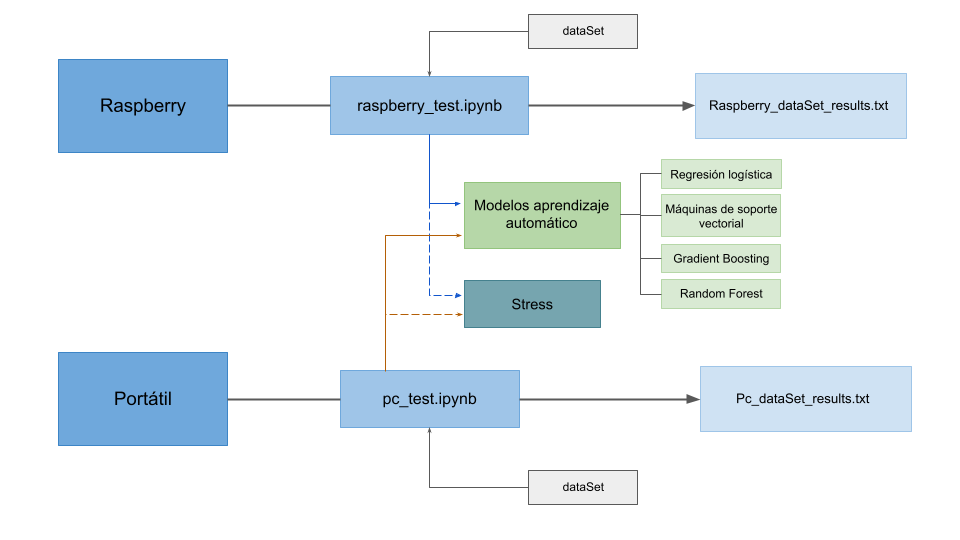
\includegraphics[width=15cm, keepaspectratio]{img/arquitectura_general.png}
  \caption{Estructura de los experimentos}\label{fig:arquitectura}
\end{figure}

Como se explicó en la sección~\ref{sec:machine_learning} hay varios tipos de aprendizaje automático y dentro de cada clase existen aún más métodos para resolver un mismo problema de formas diferentes. En este proyecto utilizaremos algoritmos de aprendizaje supervisado para realizar problemas de clasificación binaria, es decir, solo existen dos clases a las que pueden pertenecer los datos. Concretamente (y como se puede ver en la Figura~\ref{fig:arquitectura}) se utilizarán cuatro algoritmos de machine learning que son: Regresión Logística (RL), Máquinas de Vector Soporte (SVM), Gradient Boosting (GB) y Random Forest (RF).

Aprovechando los puertos GPIO de los que está provista la Raspberry Pi, en este proyecto también se utilizan un par de sensores para poder generar un nuevo \textit{dataset} con el que poder entrenar los modelos de aprendizaje automático. Estos dos sensores que se utilizan son los que se mencionaron en el apartado~\ref{sec:sensores}.

En la Figura~\ref{fig:esquema_sensores} se puede observar la estructura de como se lleva a cabo la recolección de información de los sensores por parte de la Raspberry Pi. Con todo conectado correctamente, se generará un nuevo fichero CSV con los datos medidos durante el tiempo que el usuario haya estado ejecutando el programa que se puede ver en esta figura. Este \textit{dataset} podrá utilizarse para entrenar los modelos de aprendizaje. Además, mediante la información recogida se creará una figura que contiene estos datos en cada instante de tiempo.

\begin{figure}[htb]
  \centering
  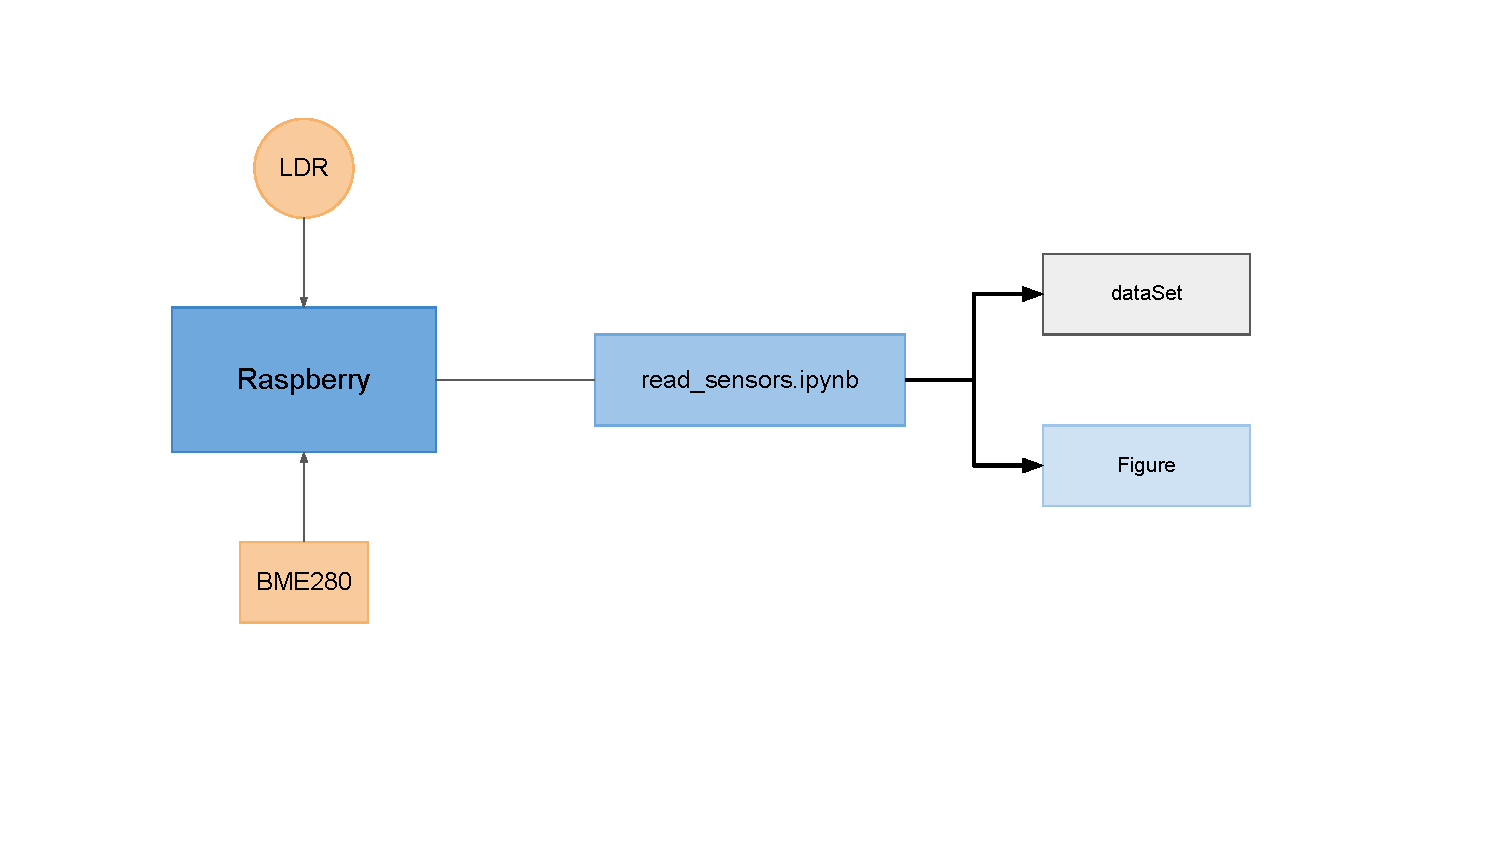
\includegraphics[width=15cm, keepaspectratio]{img/esquema_sensores.pdf}
  \caption{Estructura de creación de un nuevo de \textit{dataset} con la información de los sensores}\label{fig:esquema_sensores}
\end{figure}


\section{Configuración del entorno}
\label{sec:configuracion_entorno}

Para poder desarrollar correctamente este trabajo es necesario preparar adecuadamente el entorno, una vez acondicionado todo se dará pie al motivo principal de esta investigación.

El primer paso para esto fue montar adecuadamente la Raspberry Pi conforme las instrucciones de Okdo\footnote{\url{https://www.okdo.com/getstarted/}}, empresa de la que procede el kit con el hardware utilizado en el proyecto.

Una vez está listo el hardware, hay que instalar el software necesario para la generación de modelos de \textit{machine learning}.
Comenzando por cambiar el sistema operativo, en vez de utilizar el que viene por defecto, Raspbian Pi OS, se instaló Ubuntu 21.10\footnote{\url{https://ubuntu.com/tutorials/how-to-install-ubuntu-desktop-on-raspberry-pi-4}} para poder instalar Python 3.9, que es la versión necesaria para desarrollar los algoritmos de este proyecto.

A continuación se instaló Miniforge, por medio del cual se crea un entorno virtual donde se instalaron todos los paquetes necesarios para el proyecto como son \texttt{scikit-learn}, \texttt{Pandas}, \texttt{jupyter-notebook}... Estos paquetes permitirán desarrollar modelos de aprendizaje automático. Para mayor detalle de los paquetes instalados, en los ficheros \texttt{rasp\_enviroment.yaml} y \texttt{pc\_enviroment.yaml} se encuentran listados los paquetes que se instalaron en cada uno de los entornos creados en cada máquina.

Además se instaló \textit{stress}\footnote{\url{https://linux.die.net/man/1/stress}}, un comando de Linux que sirve para estresar durante el tiempo que se le indique el número de CPUs que se le especifican. En este caso, dicho comando se utilizará para poder someter a la Raspberry Pi a diferentes niveles de carga computacional y de este modo ver su capacidad para entrenar modelos de aprendizaje automático. Un ejemplo de ejecución de este comando es el siguiente:\\

\begin{lstlisting}[language=bash]
    $ stress -c 4 -t 120s
\end{lstlisting}

Utilizando \textit{-c} se indíca el número de CPUs que se desean estresar, que en el ejemplo anterior serán cuatro. Mientras que con \textit{-t} se indica el tiempo que van a estar los cores estresados en segundos, que en este caso son $120$ segundos.

En el Anexo (Capítulo~\ref{chap:anexo}) de esta memoria se podrá encontrar en mayor detalle las dificultades y las soluciones a los problemas hallados a la hora de realizar todo lo comentado en este apartado.


\subsection{Conexión de los sensores}
\label{subsec:conexion_sensores}

Como se comentaba en el capítulo~\ref{sec:sensores}, en este proyecto se utilizaron en total dos sensores, un LDR y un sensor BME280. Para obtener las medidas de los sensores hubo que conectar ambos tal y como se puede ver en la Figura~\ref{fig:circuito}. En esta figura el sensor de la izquierda es el BME280, mientras que en la derecha se representa el conversor HW-103 conectado al LDR.

\begin{figure}[htb]
  \centering
  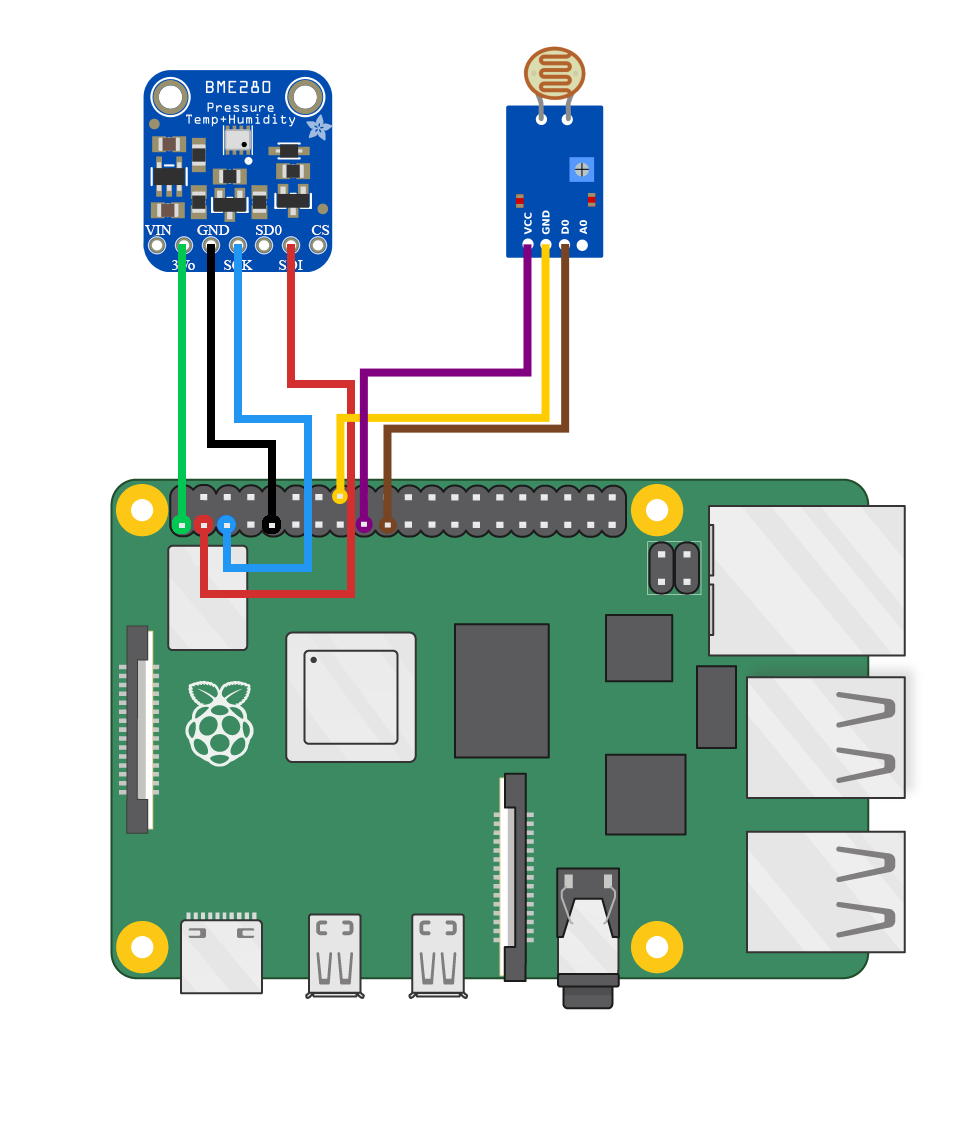
\includegraphics[width=9cm, keepaspectratio]{img/circuito.png}
  \caption{Conexiones de los sensores a la Raspberry Pi.}\label{fig:circuito}
\end{figure}

En el caso del sensor BME280 se utiliza comunicación por I2C para poder leer las medidas de temperatura, humedad y presión, por eso está conectado a los pines dos y tres de la Raspberry Pi. Mientras que el LDR se conecta al pin 10 para saber si hay luz o no.

Para poder obtener los valores del LDR fue necesario instalar el paquete LGPIO, los detalles de su instalación se encuentran en el Anexo.

Para la comunicación I2C hubo que instalar el paquete \texttt{i2c-tools} en la Raspberry Pi. Para poder utilizar este paquete es necesario tener permisos de \textit{root}, sin embargo se dieron permisos a un usuario de forma que no tuviese que ser \textit{root} para poder ejecutarlo\footnote{\url{https://lexruee.ch/setting-i2c-permissions-for-non-root-users.html}}. Dentro del entorno de Conda donde se desarrolla el proyecto se tuvieron que instalar además otros dos paquetes: \texttt{smbus2} y \texttt{RPi.bme280}. Finalizadas estas instalaciones podremos leer la información proporcionada por los sensores.

\section{Generación de los modelos de aprendizaje automático}
\label{sec:generacion_modelos}

Como se ha mencionado anteriormente, en este proyecto se utilizarán un total de cuatro algoritmos de aprendizaje automático. Los programas que se encargan de generar estos modelos se encuentran dentro de la carpeta \texttt{"Models"} de este proyecto. Hay un fichero por cada modelo que se desea entrenar y poner a prueba.

Todos estos algoritmos se han implementado utilizando la librería de \texttt{scikit-learn} que proporciona todas las funcionalidades necesarias para ello. A la hora de ejecutarlos será necesario pasarles un único argumento que es el \textit{dataset} con el que se desea entrenar el modelo.

A continuación se nombrará y se explicará brevemente el contenido de cada uno de estos ficheros.

\begin{itemize}

\item \subsubsection{lRegression.ipynb}
\label{subsubsec:lRegression}

Este fichero entrenará un modelo de Regresión Logística para el \textit{dataset} que se le pase como argumento.

En \texttt{scikit-learn}, por medio de la función LogisticRegression\cite{LogisticRegressionDoc} que pertenece a la librería \textit{sklearn.linear\_model}, se puede generar este modelo de aprendizaje automático para entrenarlo y posteriormente predecir con él. 

Entre los parámetros que se pueden asignar a esta función hay dos que son destacables. El primero de ellos es \textit{max\_iter}, máximo número de iteraciones que se permiten para encontrar la solución que converja, por defecto tiene un valor igual a $100$. En el caso de \texttt{lRegression.ipynb} se igualó el valor \textit{max\_iter} a $400$, pues es el valor mínimo necesario para que consiga encontrar una solución para algunos de los \textit{datasets} que veremos más adelante.

Por otra parte está el parámetro \textit{n\_jobs}, que permite declarar el número de CPUs que se desean utilizar para paralelizar el proceso. Sin embargo, la asignación de este valor solo tiene efecto si se realiza una clasificación multiclase, de lo contrario utilizará un único core independientemente del valor asignado. Por lo que en este caso este parámetro no se utilizará.

\item \subsubsection{svm.ipynb} 
\label{subsubsub:svm}

En esta ocasión este fichero creará un modelo de Máquinas de Vector Soporte. Para implementar este tipo de modelo de aprendizaje en \texttt{scikit-learn} se puede utilizar la función SVC \cite{SVMDocumentation}. En esta ocasión este método no soporta multiprcesamiento, por lo tanto la máquina que lo ejecute solo podrá usar un core tanto en el entrenamiento como en la predicción. 

\item \subsubsection{gBoosting.ipynb} 
\label{subsubsub:gBoosting}

Con este fichero se implementa un modelo de Gradient Boosting. En esta ocasión el método que crea este modelo es GradientBoostingClassifier\cite{GradientTreeBDoc}, que se encuentra dentro de la librería \textit{sklearn.esemble}. Al igual que para la función de Máquinas de Vector Soporte, este modelo no soporta multiprocesamiento y por lo tanto solo se utilizará una CPU para entrenar y predecir con este modelo. 
\item \subsubsection{rForest\_pc.ipynb // rForest\_pc.ipynb} 
\label{subsubsub:rForest}

Por último tendremos dos ficheros que crean un modelo basado en Random Forest.

En \texttt{scikit-learn} utilizando la función RandomForestClassifier\cite{RandomForestDoc}, que también está dentro de la librería \textit{sklearn.esemble}, se puede generar un modelo de aprendizaje utilizando esta técnica.

Para este método existe un parámetro destacable denominado \textit{n\_jobs}, que permite declarar el número de CPUs que se desean utilizar para paralelizar el proceso. Para que se note el efecto de este parámetro es necesario que el conjunto de datos con el que se desea entrenar sea grande. De lo contrario el coste de distribuir los recursos entre el número de cores indicados es más elevado que ejecutarlo todo en una única CPU, y por lo tanto los tiempos de ejecución serían más elevados a mayor número definido en este parámetro.

Por defecto si no se declara este parámetro utilizará un único core. Además se pueden asignar valores negativos, en caso de igualar \textit{n\_jobs} a $-1$ se utilizarán todos los cores disponibles en ese momento. De esta misma forma se utiliza este parámetro en Regresión Logística cuando se busca entrenar un problema de clasificación multiclase.

En esta ocasión se han creado dos ficheros para generar este modelo, puesto que dependiendo de la máquina en la que se esté ejecutando este código el valor del parámetro \textit{n\_jobs} variará. 

\end{itemize}

Estos ficheros imprimirán por el terminal cuatro valores diferentes que se utilizan para valorar la eficiencia del entrenamiento. Dichos valores son: \textit{accuracy}, \textit{accuracy trainning}, \textit{precision} y \textit{recall}. 

A continuación se detalla qué significa cada uno de esto valores. Para ello se ha definido la siguiente terminología: TP es el número de verdaderos positivos, TN verdaderos negativos, FP falsos positivos y FN falsos negativos. Siendo los valores positivos los que pertenecen a una clase y los negativos la clase contraria. En este caso diremos que los valores positivos serán los que pertenecen a la clase uno y los negativos los que pertenece a la clase cero. 

Para esta explicación nos ayudaremos de la Figura~\ref{fig:explicacion_acc}. En la cual tenemos en total dieciocho datos, diez pertenecen a la clase de los positivos (mitad izquierda de la figura) y ocho que son de la clase negativa. Los círculos grises representan donde ha colocado el modelo de ML cada dato. Como vemos ha asignado cuatro como negativos pero en realidad son positivos (zona azul claro) y tres como positivos pero pertenecen realmente a los negativos (zona verde claro).

\begin{figure}[htb]
  \centering
  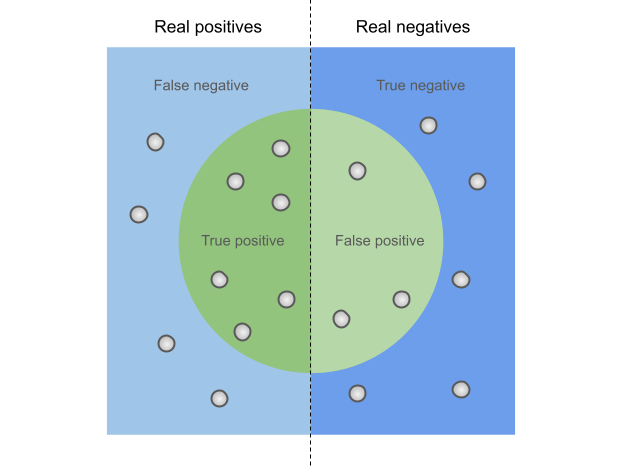
\includegraphics[width=12cm, keepaspectratio]{img/explicacion_acc.png}
  \caption{Ejemplo de estimación de un modelo \textit{machine learning}.}\label{fig:explicacion_acc}
\end{figure}

El valor de \textit{accuracy} representa el porcentaje total de aciertos. Este dato se calcula por medio de la siguiente ecuación:

\begin{equation}
 \boxed{\mbox{Accuracy} = \frac{(TP + TN)}{(TP + TN + FP + FN)}}
\end{equation}

El \textit{Trainning accuracy} es igual que el \textit{Accuracy}, lo único que cambia son los datos con los que se hacen los cálculos. Cuando se quiere obtener el \textit{Accuracy}, se utiliza un subconjunto de datos del \textit{dataset} que el modelo no ha visto durante su fase de entrenamiento. Mientras que para el \textit{Trainning accuracy}, utilizará el mismo conjunto de datos con los que ha entrenado el modelo.

\textit{Precision} es el porcentaje que se obtiene al dividir el número de positivos que ha acertado (en este caso el valor positivo, o lo que es igual, la clase uno) entre todos los positivos que se han asignado (sean correctos o no). 

Cuanto más alto sea este valor de \textit{precision} menor error habrá cometido al asignar erróneamente la clase uno. Dicho valor viene dado por:

\begin{equation}
\label{eqn:accuracy} 
 \boxed{\mbox{Precision} = \frac{TP}{(TP + FP)}}
\end{equation}

Utilizando el ejemplo de la Figura~\ref{fig:explicacion_acc}, será dividir seis (que es el número de datos dentro de el color verde oscuro) entre la suma de esos más los que están en el color verde claro.

Por último, para obtener el valor de \textit{recall} se dividen el número de verdaderos positivos entre la suma de los verdaderos positivos más los que son positivo y ha asignado como negativos. Es decir, se divide el número de veces que se ha asignado la clase uno entre la suma del número verdadero de datos que pertenecen a la clase uno más el número de veces que se ha estimado la clase cero pero en realidad los datos pertenecían a la clase uno. Siendo la fórmula por medio de la cual obtenemos este valor la siguiente:

\begin{equation}
 \boxed{\mbox{Recall} = \frac{TP}{(TP + FN)}}
\end{equation}

Según la Figura~\ref{fig:explicacion_acc} se dividirán el número de datos dentro de la zona verde oscuro entre la suma de esos más los que están en la zona azul claro.

Gracias a la librería \textit{metrics} de \texttt{scikit-learn} se pueden obtener estos valores por medio de las funciones \textit{accuracy\_score}, \textit{precision\_score} y \textit{recall\_score}. 

Pero para obtener estos valores es necesario ejecutar primero la función \textit{predict} a la que se le pasa como argumento el set de datos del que se desea realizar una predicción. Al ejecutarlo devolverá las salidas que ha estimado el modelo para cada una de las entradas, esto se puede ver en el Código~\ref{lst:get_APR}. Esta salida se les pasa como segundo a las funciones mencionadas antes, y como primer argumento necesitan las salidas verdaderas de los datos con los que se ha hecho la predicción. 

Salvo en el caso de \textit{trainning accuracy}, habrá que utilizar las predicciones hechas sobre las entradas del \textit{dataset} que se utilizan para probar el modelo. Para el \textit{accuracy trainning} necesitaremos las predicciones de los datos con los que ha entrenado el propio modelo.

\begin{listing}[htb]
    \caption{Obtención de los valores de Accuracy, Trainning accuracy, Precision y Recall.}{}
    \label{lst:get_APR}
    \begin{minted}[breaklines, fontsize=\footnotesize, baselinestretch=1]{python}
occup_pred_train= l_regr.predict(x_scaled)
occup_pred = l_regr.predict(x_test_scaled)    
label= y[0]

accuracy = metrics.accuracy_score(y_train, occup_pred_train)*100
print("Trainning Accuracy: ","{:.1f}".format(accuracy),"%")

accuracy = metrics.accuracy_score(y_test, occup_pred)*100
print("Accuracy: ","{:.1f}".format(accuracy),"%")
precision = metrics.precision_score(y_test, occup_pred, pos_label=label)*100
print("Precision: ","{:.1f}".format(precision),"%")
recall = metrics.recall_score(y_test, occup_pred, pos_label=label)*100
print("Recall: ","{:.1f}".format(recall),"%")
    \end{minted}
\end{listing}

Como se puede ver en el Código~\ref{lst:get_APR} para los valores de \textit{Precision} y \textit{Recall} se pasa un tercer parámetro, que es la clase respecto a la que se desea calcular dichos valores. Ya que en vez de calcularlos para la clase positiva (como hemos visto anteriormente) se podrían calcular también respecto de la clase negativa.

\section{Dataset: Room Occupacy}
\label{sec:dataSet_Occupancy}

Para realizar la clasificación en un inicio se utilizó el data set de Room Occupancy detection data\cite{DataSetOccupancy}, obtenido de Kaggle, que contiene unas 20.560 muestras. Tal y como su nombre indica, este \textit{dataset} proporcionará información sobre si una habitación se encuentra en un determinado instante ocupada o no. Cada ejemplo tiene las medidas de temperatura, humedad, CO2 y luz de una habitación de oficina de unos quince metros cuadrados. La última columna de cada fila indica la clase a la que pertenece la muestra. En este caso, al ser una clasificación binaria esta última columna solo puede tener dos valores, cero o uno. Si para un ejemplo contiene un uno significa que para esos valores la habitación está ocupada. Si por el contrario hay un valor de cero la sala está vacía. 

Este \textit{dataset} se encuentra en la carpeta \texttt{"occupancy"} del repositorio\footnote{\url{https://github.com/Nuriadj/TFG}} con el nombre \texttt{occupancy\_clean.csv} puesto que para poder utilizar el \textit{dataset} había que eliminar tanto la cabecera como la primera columna del set de datos original (\texttt{occupancy.csv}).

% Antes de poder utilizar este \textit{dataset} para poder entrenar modelos, es necesario hacer un preprocesamiento quitándole la primera columna que son las fechas de los datos, columna que no es relevante para entrenar los modelos. Y también hay que quitarle la cabecera.

Para generar los modelos se dividió el set de datos en dos partes, una primera parte para entrenar (que contenía el $70\%$ de ejemplos del set de datos original) y otra para comprobar la eficiencia del modelo a la hora de clasificar si la estancia está ocupada o no (es decir, un set de datos de prueba). En esta segunda parte se utilizó el $30\%$ restante de muestras del set de datos original, que no se utilizaban en el entrenamiento y por lo tanto el modelo nunca los había visto, son totalmente nuevos para él.

Un aspecto importante a destacar de este set de datos es que hay una mayor cantidad de ejemplos de habitación no ocupada que de ocupada. En otros \textit{datasets} esto podría representar un problema ya que puede dar lugar a que al realizar esta división de forma aleatoria, el conjunto de datos de entrenamiento apenas tenga ejemplos de una de las clases. Sin embargo, al tener una gran número de ejemplos en el que ambas clases tienen una gran cantidad de muestras, como es este caso, una división aleatoria no representa ningún inconveniente dado que hay una alta probabilidad de que el set de entrenamiento siempre tenga como mínimo la cantidad de muestras necesarias de ambas clases para entrenar correctamente. Aun así, la división se realizó de forma estratificada, para que hubiese la misma proporción de datos de una clase u otra, que en el set de datos original. Y de esta forma nos aseguramos que a la hora de entrenar, como de comprobar el modelo generado, se tengan ejemplos de ambas clases en la misma proporción que aparecen en el set de datos original.

Con esta división y preparación de los datos, los cuatro modelos se pudieron generar sin problemas utilizando los programas que se encuentran dentro de la carpeta \texttt{"Models"}. 


\subsection{Validación cruzada}

Para comprobar mejor la calidad de los modelos se utilizó validación cruzada. La validación cruzada consiste en hacer que dentro del set de datos de entrenamiento (en este caso compuesto, una vez más, por el $70\%$ de ejemplos del set de datos original) se realiza una subdivisión en otros cinco sets (en el caso de este proyecto). Lo más común es dividir el set de datos de entrenamiento en diez \textit{subdatasets}, pero se decidió utilizar únicamente cinco puesto que se consideraron suficientes para observar la eficiencia que ha tenido el modelo al entrenar. 

Para ello, se utilizan dos métodos el primero de ellos es \textit{KFold} que devuelve los índices por donde se van a dividir los datos para obtener varios sets (el número de sets dependerá del valor que se le asigne al parámetro \textit{n\_splits}). La segunda función que se utiliza es \textit{cross\_val\_score}, a la que se le pasa el modelo que se quiere probar junto con los datos de entrenamiento y los índices obtenidos por \textit{KFold}. Esta función nos devolverá el \textit{Accuracy} que ha conseguido cada uno de estos \textit{subdatasets}.

Una vez realizada la división se entrena con todo el \textit{dataset} de entrenamiento y se vuelve a comprobar la eficiencia (de ese modelo entrenado) con el $30\%$ de datos de la división original, los que nunca ha visto ni entrenado con ellos.

El objetivo de realizar una validación cruzada es garantizar que los resultados que obtengamos sean independientes de la partición entre datos de entrenamiento y datos de validación. Es decir, poder saber si la precisión que obtenemos al hacer la predicción es real o se ha sobreajustado a un \textit{dataset} concreto.
 
 Para utilizar validación cruzada se añadió a los ficheros de la carpeta \texttt{"Models"} los métodos mencionados anteriormente. Por lo que, además de los datos que ya mostraban estos ficheros por su salida, se añadirá un nuevo \textit{print} para obtener la media total de las precisiones de cada una de las subdivisiones, mostrándolo con la etiqueta \textit{"Mean Folds Accuracy"} por ser la media del resultado obtenido en cada \textit{"Fold"}. En el Código~\ref{lst:get_CV} se pueden ver las líneas añadidas al Código~\ref{lst:get_APR} para incluir esta funcionalidad.
 
 \begin{listing}[htb]
    \caption{Obtención de la precisión media de cada uno de los \textit{subdatasets} de la validación cruzada.}{}
    \label{lst:get_CV}
    \begin{minted}[breaklines, fontsize=\footnotesize, baselinestretch=1]{python}
#Validacion cruzada
kfold = KFold(n_splits=5, shuffle=True)\n",
acc_folds = cross_val_score(l_regr, x_scaled, y_train, cv=kfold)

print(\"Mean Folds Accuracy: \",\"{:.1f}\".format(acc_folds.mean()*100),\"%\")
    \end{minted}
\end{listing}
 


\section{Dataset: KddCup99}
\label{subsec:dataset_kddcup99}

Al realizar algunas pruebas para observar el comportamiento de la Raspberry Pi ante diferentes situaciones de estrés (tal y como se explicará más adelante) los resultados obtenidos no encajaban del todo con lo esperado. Para tratar de comprender mejor lo que estaba pasando se decidió usar un \textit{dataset} más grande que el anterior.

El \textit{dataset} elegido fue KDD Cup 1999 Data\cite{DataSetKddCup99}, obtenido una vez más desde la página web de Kaggle. Este \textit{dataset} se utilizó en el tercer concurso internacional de herramientas de descubrimiento de conocimientos y minería de datos, el objetivo del concurso era generar un modelo predictivo que fuese capaz de distinguir entre conexiones \textit{"malas"}, es decir, intrusiones o ataques, y conexiones \textit{"buenas"}. Este set de datos contiene una gran variedad de intrusiones en un entorno de red militar. 

De este \textit{dataset} se utilizó tanto el fichero \texttt{kddcup.data.gz} como \\\texttt{kddcup.data\_10\_percent.gz}. Una vez descargados se descomprimen y se ejecuta un programa, llamado \texttt{prepare\_kddcup.ipynb}, para tratar los datos que contienen y poder utilizarlos en la generación de los modelos de ML.

Al igual que en el \textit{dataset} de Room Occupancy para la generación de los modelos se utilizará el $70\%$ de los datos para entrenar y el $30\%$ para validar.

\subsection{Preprocesamiento de KddCup99}
\label{subsec:preprocesamiento_kddcup}

Para que este \textit{dataset} se pueda utilizar para entrenar a modelos de aprendizaje automático de clasificación binaria, es necesario realizar un preprocesamiento a los datos que contiene~\cite{Pyle1999,Dasu2003}. De esto se encarga el programa \texttt{prepare\_kddcup.ipynb}. Este fichero permite leer las líneas de este \textit{dataset}, procesar y guardar los datos en un nuevo fichero para que puedan usarlos los modelos.

Para leer los datos se utiliza la función \textit{read\_csv} de \texttt{Pandas}. Este programa no solo se utilizará para leer un \textit{dataset} al completo, sino que también podremos leer otra porción diferente de líneas. Es por esto que para que el programa ejecute correctamente hay que pasarle un número como único argumento, cuyo valor puede estar entre cero y cien. Este valor representa el porcentaje de datos que se desea leer. Un ejemplo de ejecución de este fichero para que lea el $50\%$ de los datos de KddCup99 es:\\

\begin{lstlisting}[language=bash]
    $ ipython prepare_kddcup.ipynb 50
\end{lstlisting}

En el caso de \texttt{kddcup.data} (que contiene más de un millón de líneas) interesa poder leer diferentes cantidades de datos del fichero puesto que tanto la Raspberry Pi como el portátil no son capaces de leer este \textit{dataset} al completo, los procesos morían antes de terminar. En el caso de la Raspberry Pi el máximo de datos que es capaz de leer, sin que muera el proceso, es el cuarenta porciento del \textit{dataset} total mientras que el portátil llegaba al cincuenta porciento del total.

Para leer otro porcentaje del \textit{dataset} total, que no fuese únicamente el diez porciento, se utiliza una regla de tres. Sabiendo que el diez porciento del set de datos (el fichero \texttt{kddcup.data\_10\_percent}) contenía $494.020$ líneas, se podía obtener aproximadamente a cuantas líneas equivaldría otro porcentaje como la cantidad total de líneas que debía tener el \textit{dataset} completo.

La función \textit{random.sample} devuelve una lista que contiene valores numéricos aleatorios, para realizar esta función es necesario que se le pasen dos argumentos. El primero de ellos es el valor máximo que puede aparecer en la lista, siendo el mínimo igual a cero. El segundo argumento es la longitud total de la lista, es decir, cuántos números aleatorios va a generar. Con este método se obtendrá una lista con valores aleatorios que se le asignará al parámetro \textit{skiprows} de \textit{read\_csv}. Haciendo que todos esos datos, que representan números de líneas del fichero original, no se lean, consiguiendo hacer que se lea únicamente el porcentaje que ha pedido el usuario.

La implementación de cómo se lee un porcentaje concreto del \textit{dataset} se puede ver en el Código~\ref{lst:prepare_kddcup}, donde \textit{total} es el valor máximo de líneas que hay en el fichero \texttt{kddcup.data} (obtenido mediante la regla de tres comentada anteriormente), \textit{per\_lines} es el número de líneas que sí se desean leer (obtenido al aplicar una regla de tres al porcentaje que se ha pasado como argumento a \texttt{prepare\_kddcup.ipynb}). Ambos valores los usa \textit{random.sample} para obtener líneas aleatorias, que se ordenarán utilizando \textit{sorted} para poder pasárselas a \textit{skiprows}, y que por lo tanto no se leerán.

\begin{listing}[htb]
    \caption{Lectura del \textit{dataset} y conversión a clase binaria.}{}
    \label{lst:prepare_kddcup}
    \begin{minted}[breaklines, fontsize=\footnotesize, baselinestretch=1]{python}
#Obtener número de lineas a leer
total= 4940200 # numero de lineas aproximado del fichero kddcup.data
per_lines= int((float(sys.argv[1])*total)/100)
#Leer dataSet
rm_lines= sorted(random.sample(range(total),total-per_lines))
dataset = pd.read_csv('/home/nuriadj/Documents/TFG/kdd_cup99/kddcup.data', skiprows=rm_lines)
print("Reading: %2.f" % round((len(dataset)*100)/total,2),"% of the csv")

#Conversión multiclase a binaria
dataset['normal.'] = dataset['normal.'].replace(['back.', 'buffer_overflow.', 'ftp_write.', 'guess_passwd.', 'imap.', 'ipsweep.', 'land.', 'loadmodule.', 'multihop.', 'neptune.', 'nmap.', 'perl.', 'phf.', 'pod.', 'portsweep.', 'rootkit.', 'satan.', 'smurf.', 'spy.', 'teardrop.', 'warezclient.', 'warezmaster.'], 'attack')
    \end{minted}
\end{listing}

Otro aspecto relevante de este \textit{dataset} es que contiene datos que pertenecen a varias clases. Por lo tanto, dado que estamos resolviendo problemas de clasificación binaria, habrá que hacer un tratamiento previo a la información que contiene el \textit{dataset} para que se puedan agrupar los datos en dos clases en vez de en múltiples.\\
Este programa también hace esta conversión de multiclase a dos clases. Para ello, una vez leídos todos los datos se reemplazaban todas las clases (excepto la clase \textit{"normal."}) por la clase \textit{"attack"}\cite{MulticlassToBinary}, de esta forma se consigue tener solo dos clases. El código que realiza esta tarea se puede ver en el Código~\ref{lst:prepare_kddcup}.

Una vez realizada la transformación de multiclase a clase binaria, se hace un pequeño tratamiento a los datos para que cada modelo pueda entrenar adecuadamente y más fácilmente con ellos\cite{dataSetTreatment}. Para ello se elimina la columna $19$ y $20$, ya que estas solo contienen un único valor, que es cero. A continuación se transforman los datos categóricos y por último se eliminan las filas duplicadas. Con este tratamiento los datos se guardan utilizando la función \textit{to\_csv} que proporciona \texttt{Pandas} y se guarda el nuevo set de datos tratados sin la cabecera ni el índice, de forma que desde el código de cada uno de los modelos los datos estén listos para poder ser utilizados.

En el repositorio de este proyecto dentro de la carpeta \texttt{"kdd\_cup99"} se pueden encontrar varios CSV con diferentes porcentajes de datos, listos para ser utilizados solo hay que descomprimirlos.

\section{Dataset: Sensores Raspberry Pi}
\label{sec:mi_dataSet}

A parte de los \textit{datasets} anteriores se creó uno utilizando la información recopilada por lo sensores, mediante el programa \texttt{read\_sensors.ipynb}. Este \textit{dataset}, con medidas de temperatura, humedad, presión y luz, busca generar un modelo que nos permita saber si la habitación está ocupada o no en un determinado instante de tiempo, al igual que sucedía con el \textit{dataset} de Room Occupancy. En la Figura~\ref{fig:mi_setup} se puede observar de qué forma estaban dispuestos los diferentes componentes \textit{hardware} para poder generarlo.

\begin{figure}[htb]
  \centering
  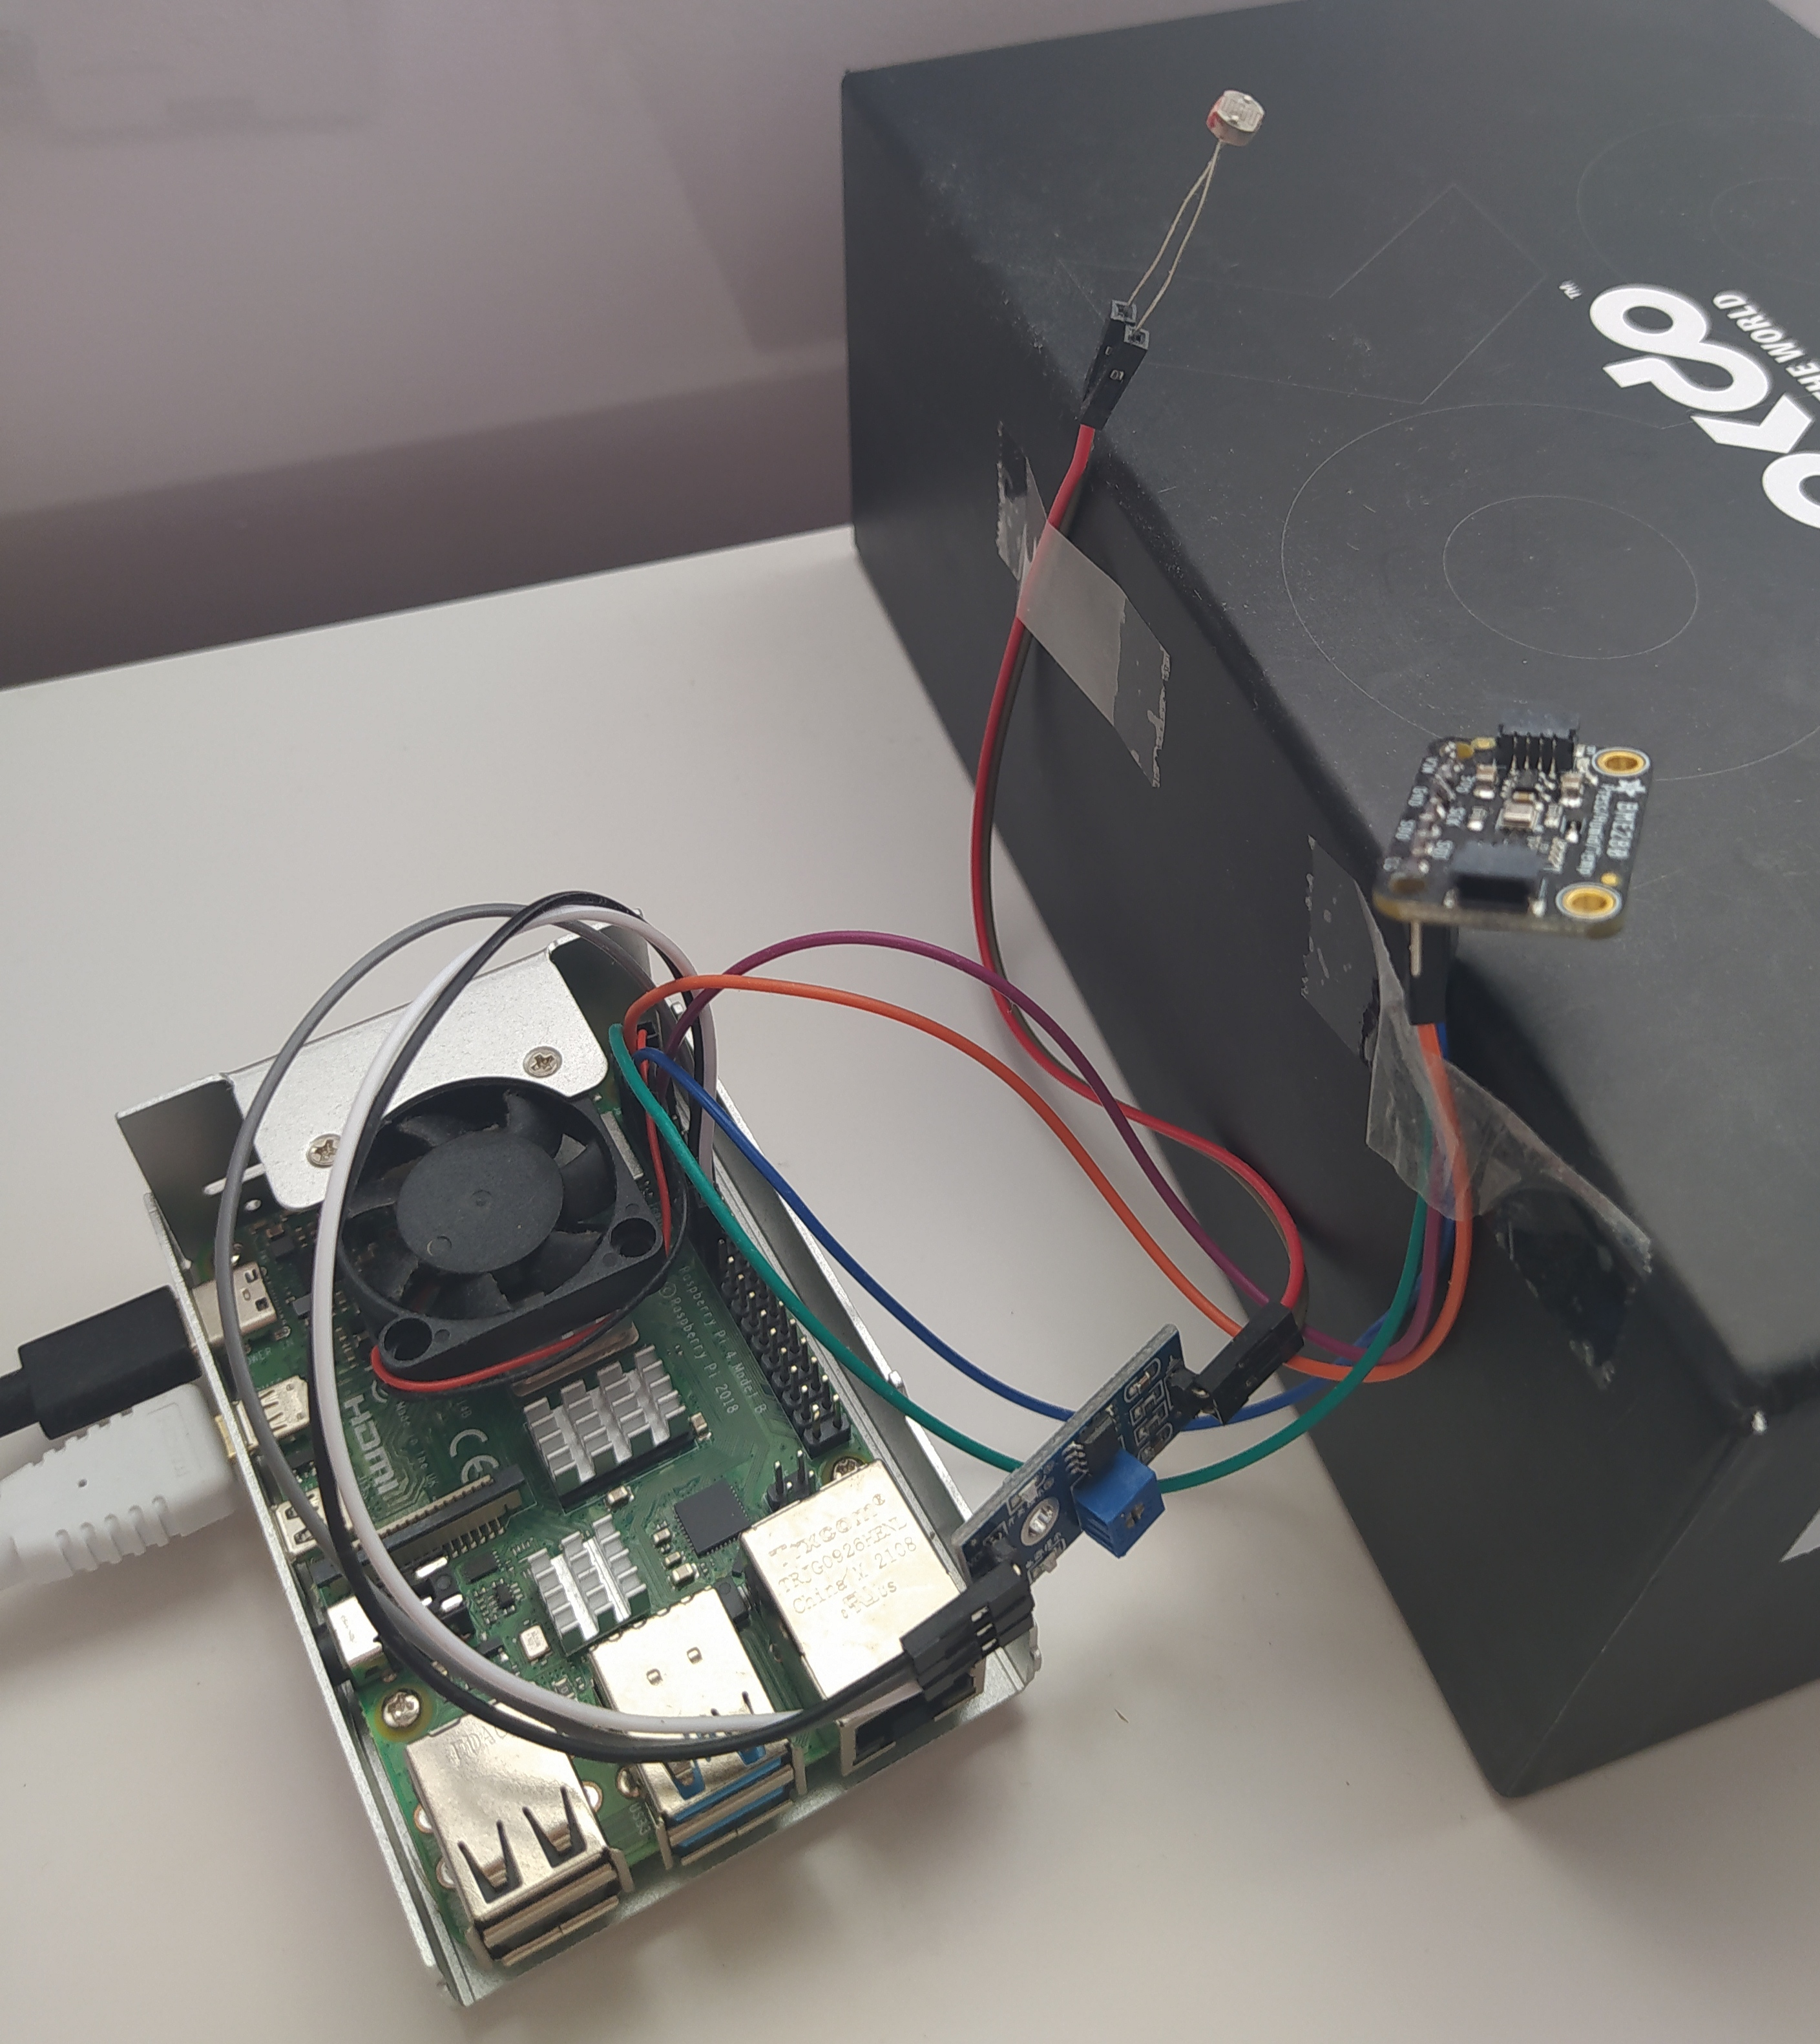
\includegraphics[width=8cm, keepaspectratio]{img/mi_setup.jpg}
  \caption{\textit{Setup} del \textit{hardware} para tomar las medidas de los sensores.}\label{fig:mi_setup}
\end{figure}

 Para crear el set de datos, durante varias horas se tomaban medidas en una habitación, de forma controlada, es decir, sabiendo en cada instante si la habitación estaba ocupada o no. Cuando la habitación estaba vacía algunas veces se cerraba la persiana de la ventana de la habitación para que también tomase medidas bajo esta nueva condición.

Una vez finalizado el tiempo que se deseaba hacer la prueba se paraba el programa \texttt{read\_sensors.ipynb}, se abría el nuevo CSV generado y se añadía una nueva columna que representa el estado de la habitación en cada instante, asignando un uno cuando estaba ocupada y un cero en el caso contrario.

\subsection{read\_sensors.ipynb}
\label{subsec_read_sensors}

Como se ha comentado anteriormente este programa es el encargado de tomar las medidas de los sensores conectados a la Raspberry Pi, guardarlas y generar con ellas un nuevo CSV y una imagen que muestra de forma gráfica los valores obtenidos en cada instante de tiempo, de modo que sea más fácil interpretar lo que ha pasado en ese periodo de tiempo. 

Para que pueda ejecutar correctamente es necesario que se le pase como argumento el nombre con el que se desea guardar el \textit{dataset} que se va a generar. Este argumento también se utilizará para nombrar la gráfica que genera el programa con el siguiente formato: \texttt{Data\_graph\_miDataSet}, siendo miDataSet el \textit{string} que se ha pasado como argumento.

Este programa necesita usar la comunicación I2C para obtener los valores del sensor BME280 pero también necesitará acceder directamente a los pines por medio de la librería LGPIO. Para poder utilizar LGPIO es necesario ejecutar el programa con permisos de \textit{root} pero manteniendo el entorno Conda actual (pues es donde se encuentran todas las librerías instaladas), es por ello que para ejecutarlo habrá que utilizar la siguiente línea de comando: \\

\begin{lstlisting}[language=bash]
    $ sudo env "PATH=$PATH" ipython read_sensors.ipynb miDataSet
\end{lstlisting}

En la segunda celda de este programa se puede ver cómo se prepararán los puertos para poder leer los datos. 

A continuación se quedará ejecutando indefinidamente un bucle \textit{while}, que es el que se encarga de guardar los datos detectados por los sensores cada segundo. Dicho bucle se puede ver en el Código~\ref{lst:firstloop_read_sensor}. Algo destacable es que para obtener el valor de la luz (proporcionada por el LDR) siempre se le resta a uno el valor obtenido por el LDR. Esto se hace así para que los datos se puedan interpretar mejor, puesto que cuando hay luz a la Raspberry Pi le llega un cero. De esta forma cuando haya luz se guarda un uno en el fichero en vez de un cero. 
Este bucle estará continuamente mostrando por el terminal las medidas tomadas hasta que el usuario haga Ctr-C , de esta forma se indica que ya no se desean guardar más datos.

\begin{listing}[htb]
    \caption{Bucle que guarda los datos detectados por los sensores.}{}
    \label{lst:firstloop_read_sensor}
    \begin{minted}[breaklines, fontsize=\footnotesize, baselinestretch=1]{python}
measures= [] #array que contiene los valores del sensor

try:
    while True:

        bme280_data = bme280.sample(bus, address)
        humidity= bme280_data.humidity
        pressure= bme280_data.pressure
        temp= bme280_data.temperature
        
        light= lgpio.gpio_read(h, LDR)
        light= 1 - light
        
        measures.append([humidity, pressure, temp, light])
        
        print(humidity, pressure, temp, light)
        time.sleep(1)
except KeyboardInterrupt:
   pass  
    \end{minted}
\end{listing}

Una vez que este bucle ha finalizado, se ejecuta otro que iterará sobre los datos guardados en la lista \textit{measures} para poder pintar esos valores en la gráfica que devuelve este programa. Dicho bucle se puede ver en el segmento del Código~\ref{lst:secondloop_read_sensor}. Hay dos cosas destacables de este trozo de código. La primera es que el valor de las presiones se divide entre diez, esto se debe a que las presiones que devuelve el sensor BME280 son valores muy superiores a los que puede conseguir cualquiera de los otros sensores, por lo que en vez de devolver la medida en $hPa$ se divide entre diez para obtenerla en $KPa$ y de esta forma poder apreciar mejor los cambios en los datos de todos los sensores.

El segundo aspecto destacable es sobre el valor de la luz, que se multiplica por cincuenta. Al igual que en el caso de las presiones esto se hace para que el cambio de estado entre oscuridad y luz sea apreciable en la gráfica, de lo contrario el salto entre ceros y unos apenas se podrían ver.

\begin{listing}[htb]
    \caption{Bucle para generar la gráfica.}{}
    \label{lst:secondloop_read_sensor}
    \begin{minted}[breaklines, fontsize=\footnotesize, baselinestretch=1]{python}
hum= []
temp= []
pres= []
light= []
x= []

for i in range(len(measures)):
    hum.append(measures[i][0])
    pres.append(measures[i][1]/10)
    temp.append(measures[i][2])s
    light.append((measures[i][3]*50))#multiplico por 50 para verlo mejor en el plot
    x.append(i)
    \end{minted}
\end{listing}

Mediante todo esto se obtuvo un nuevo \textit{dataset} denominado como \texttt{occup\_detec\_2h.csv}. A este \textit{dataset} se le añadió una nueva columna para indicar en qué instantes de tiempo la habitación estaba ocupada o vacía, y por ello se guardó con el siguiente nombre: \texttt{occup\_detec\_2h\_Clean.csv}, para de esta forma indicar que el \textit{dataset} estaba listo para poder entrenar modelos con él.

La gráfica generada por este \textit{dataset} se puede observar en la Figura~\ref{fig:ejemplo_gráfica}. Donde el eje x representa los minutos que han pasado desde que comenzó a ejecutarse el código.

\begin{figure}[htb]
  \centering
  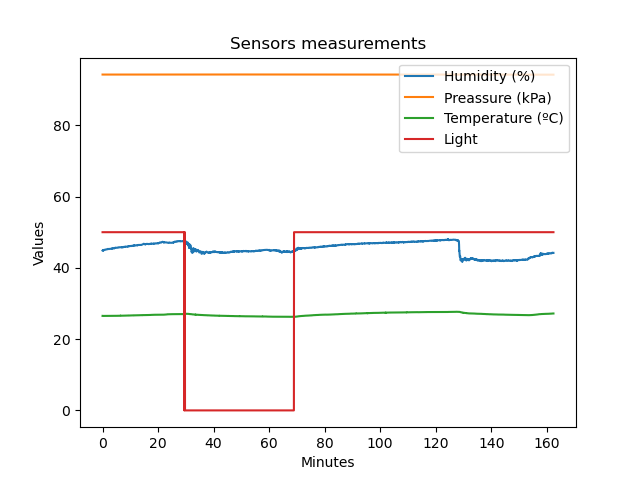
\includegraphics[width=11cm, keepaspectratio]{img/Data_occup_detec_2h_original.png}
  \caption{Ejemplo gráfica de las medidas de los sensores.}\label{fig:ejemplo_gráfica}
\end{figure}

Para la generación de este set de datos se utilizó una habitación de unos ocho metros cuadrados, donde primero estuvo ocupada durante media hora. Pasada esa media hora la habitación estuvo vacía durante 40 minutos. Después volvió a estar ocupada durante una hora entera, se vació una última vez durante 25 minutos para estar ocupada los 10 últimos minutos antes de finalizar la recogida de datos.

Sabiendo en qué momentos ha estado ocupada o vacía y observando la Figura~\ref{fig:ejemplo_gráfica} se puede ver que los valores de los datos varían entre el estado ocupado y vacío (a excepción de la presión que no cambia), siendo la humedad la variable donde más se diferencian los valores entre ambos estados. La temperatura varia algo menos, pero igualmente se puede ver un pequeño descenso cuando la habitación está vacía. En la Figura~\ref{fig:graf_temp} podemos ver en mayor detalle el valor de la temperatura en cada instante de tiempo.

\begin{figure}[htb]
  \centering
  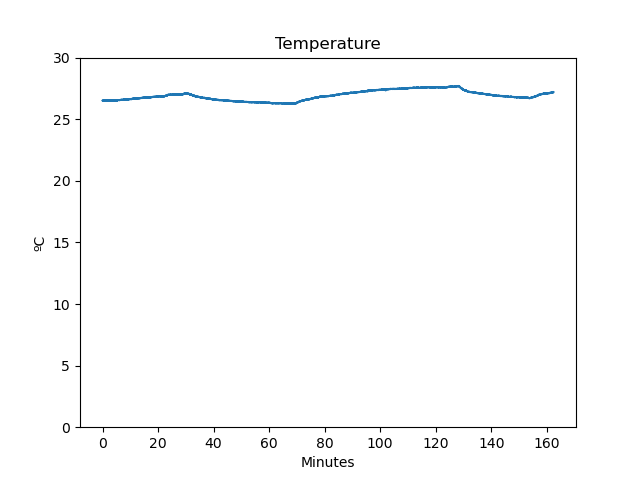
\includegraphics[width=10cm, keepaspectratio]{img/Temp_occup_detec_2h_original.png}
  \caption{Gráfica de la temperatura para el \textit{dataset} \texttt{occup\_detec\_2h\_Clean.csv}}\label{fig:graf_temp}
\end{figure}

\cleardoublepage

%%%%%%%%%%%%%%%%%%%%%%%%%%%%%%%%%%%%%%%%%%%%%%%%%%%%%%%%%%%%%%%%%%%%%%%%%%%%%%%%
%%%%%%%%%%%%%%%%%%%%%%%%%%%%%%%%%%%%%%%%%%%%%%%%%%%%%%%%%%%%%%%%%%%%%%%%%%%%%%%%
% EXPERIMENTOS Y VALIDACIÓN %
%%%%%%%%%%%%%%%%%%%%%%%%%%%%%%%%%%%%%%%%%%%%%%%%%%%%%%%%%%%%%%%%%%%%%%%%%%%%%%%%

\chapter{Experimentos y validación}
\label{chap:experimentos}

En este capítulo comprobaremos la eficiencia de la Raspberry Pi a la hora de generar los modelos de aprendizaje automático para que se ajusten los \textit{datasets} mencionados en el capítulo anterior. Las pruebas consistirán en someter a la máquina a diferentes niveles de cargas computacionales para observar como lidia la Raspberry Pi con la generación del modelo a la vez que con estas cargas.
Además ejecutaremos las mismas pruebas en un portátil para poder comparar los resultados de ambos dispositivos.

\section{Estructura de los experimentos}
\label{sec:estructura_experimentos}

Para realizar los experimentos se definieron cuatro niveles de saturación, dependiendo del dispositivo en el que se ejecuten, las pruebas variarán un poco. 

El primer nivel es el \textit{Idle} en el que no se somete a la máquina a ningún tipo de carga extra, esto es igual en ambos dispositivos. Salvo este primer nivel, el resto sí variarán ligeramente entre ambas máquinas.

En el caso de la Raspberry Pi el nivel bajo consiste en estresar una única CPU, el nivel medio dos CPUs y por último en el nivel alto se estresaban todas las CPUs de la Raspberry Pi, es decir, cuatro CPUs. 

Mientras que en el portátil, dado que este tiene un total de ocho CPUs físicas, la cantidad de carga computacional a la que se somete en los niveles bajo, medio y alto, cambia para poner más o menos en la misma situación a ambas máquinas. Por lo tanto en este caso el nivel bajo de carga será estresar dos de sus CPUs, el nivel medio cuatro y el alto los ocho cores de los que dispone la máquina. De esta forma se podrán comparar los tiempos de ejecución en un dispositivo de mayor capacidad y sabremos cuanto dista el comportamiento de la Raspberry Pi del de una máquina con mayor potencia.

Cada uno de los códigos encargados de generar uno de los modelos, es decir cada fichero que se encuentra dentro de la carpeta \texttt{"Models"}, se ejecuta con estos cuatro niveles de carga. Para generar esta carga se usa el comando \textit{stress} que permite estresar, durante el tiempo que se le indique, el número de CPUs que se le comanden. 

Una de las medidas que se utilizan para comparar los diferentes niveles de estrés es el tiempo que tarda cada uno de los modelos en terminar de ejecutar. Para obtener dicho tiempo se utiliza el comando \textit{time} de Linux, con el que se ejecuta cada modelo de la siguiente forma:\\

\begin{lstlisting}[language=bash]
  $ time ipython modelo.ipynb
\end{lstlisting}

El comando \textit{time} devuelve tres valores. Uno de ellos es el tiempo de usuario, que es la cantidad de tiempo que ha gastado el proceso en modo usuario. El \textit{Sys time} es el tiempo de CPU invertido en el kernel por el proceso. Con estos dos tiempos se puede obtener el \textit{CPU time}, el tiempo total que ha utilizado la CPU para completar la ejecución del proceso. Por otra parte \textit{time} también proporciona el \textit{real time}, que es el tiempo que ha tardado en ejecutar el proceso como si lo hubiésemos cronometrado con un reloj, este tiempo es el mismo que el \textit{Wall time}. 

Además, la relación que haya entre \textit{CPU time} y \textit{Wall time} nos indicará si se están ejecutando procesos en paralelo o no. En el caso de que el \textit{Wall time} y el \textit{CPU time} sean similares significará que no se están paralelizando los procesos. Mientras que si el \textit{CPU time} es mayor que el \textit{Wall time} sí que se estarán ejecutando procesos en paralelo\cite{timeDoc}. Es necesario entender todo esto para poder comprender los valores que nos devolverán los experimentos.

Esto junto con los valores de \textit{Accuracy}, \textit{Trainning Accuracy}, \textit{Precision}... Son los valores que se utilizarán en todas las pruebas para evaluar el comportamiento tanto de la Raspberry Pi como de los modelos generados.

\subsection{Ejecución de los experimentos}
\label{subsec:ejecucion_experimentos}

Para realizar todas las pruebas, tal y como se ha explicado, se creó un programa para cada una de las máquinas de forma que fuese más sencillo obtener los resultados de los experimentos. En el caso de la Raspberry Pi este programa se denominó \texttt{raspberry\_test.ipynb}. En el caso del portátil se nombró \texttt{pc\_test.ipynb}. Dado que las pruebas en ambos dispositivos son prácticamente las mismas, sólo existen pequeñas diferencias entre ambos programas.

Dichos programas necesitan como único argumento el \textit{dataset} con el que se desea hacer el experimento para que puedan realizar su función correctamente.
Hay que tener en cuenta que este \textit{dataset} debe de estar limpio, es decir, que se le haya hecho un preprocesamiento para borrar características no deseadas o redundantes. Tampoco debe de tener cabecera. Si no se hace este preprocesamiento podrá dar error la ejecución.

A continuación se desarrollará en mayor profundidad qué es lo que hace cada programa para realizar las pruebas.


\subsubsection{raspberry\_test.ipynb}
\label{subsubsec:programa_pruebas_raspberry}

La misión de este código es ejecutar cada uno de los modelos de aprendizaje automático (que se utilizan en este proyecto), con los diferentes niveles de saturación comentados anteriormente, en la Raspberry Pi. Para realizar esto se usan dos bucles anidados, el primero de ellos itera sobre los modelos que se desean poner a prueba. El segundo recorre una lista que contiene el número de cores que se desean estresar con cada uno de los modelos, ambos bucles los podemos ver en el Código~\ref{lst:funcion_principal_raspberry_test}. Si el valor sobre el que se está iterando de la lista es mayor que cero significa que se desea estresar cierto número de CPUs, por lo tanto se llama a la función \textit{start\_stress} a la que se le pasa como argumento el número de procesadores a estresar y durante cuanto tiempo, con estos datos se encargará de crear un nuevo proceso para ejecutar el comando \textit{stress}.

Por otra parte, independientemente del nivel de saturación de la prueba, siempre se llamará a la función \textit{model} que creará un nuevo proceso para ejecutar, utilizando el comando \textit{time} de Linux, uno de los ficheros que se encuentran dentro de la carpeta \texttt{"Models"}. Cada uno de los ficheros que se encuentran dentro de dicha carpeta generará uno de los modelos de aprendizaje automático que se han explicado en este proyecto. 

\begin{listing}[htb]
    \caption{Función principal raspberry\_test.ipynb}{}
    \label{lst:funcion_principal_raspberry_test}
    \begin{minted}[breaklines, fontsize=\footnotesize, baselinestretch=1]{python}
t= 2000
list_cpus= [0,1,2,4]
dataSet= sys.argv[1]
name_dataSet= dataSet.split("/")[-1].split(".csv")[0]
folder_name= name_dataSet+"_raspresults"

#Crear la carpeta
if(os.path.exists("./"+folder_name)== False):
    os.mkdir(folder_name)
name_dataSet= "./"+folder_name+"/"+name_dataSet

lst_header= []
lst_Wt= []
lst_Ct= []
lst_Af= []
lst_TAc= []
lst_Ac= []
lst_Pr= []
lst_Re= []

for i in range(4):
    for j in list_cpus:
        num_cores= j
        
        if(j > 0):
            pid_stress= start_stress(j, t)
        else:
            print("\nCpu Idle")
            
        model_num= i    
        model(model_num)
        
        if j > 0:
            os.killpg(os.getpgid(pid_stress.pid), signal.SIGKILL)
        
        print("Sleeping for 5 sec...\n")
        time.sleep(5)
    \end{minted}
\end{listing}

Cuando se completa la generación del modelo para uno de los niveles, los resultados de \textit{CPU time}, \textit{Wall time}, \textit{Mean Folds Accuracy}, \textit{Accuracy trainning}, \textit{Accuracy}, \textit{Precision} y \textit{Recall} se guardan cada uno en su respectiva lista gracias a una función del programa llamada \textit{get\_data}. Una vez que uno de los modelos ha completado todas las pruebas se genera un nuevo fichero CSV, mediante la función \textit{add\_data}, con los resultados obtenidos en cada uno de los casos.
Este fichero tendrá por nombre el siguiente formato: \texttt{nombreDataSet\_raspMD.csv}, donde MD son las siglas del modelo que se ha ejecutado. Por ejemplo, en el caso de Regresión Logística el nombre será \texttt{nombreDataSet\_raspLR.csv}, o en el caso de Máquinas de Vector Soporte será \texttt{nombreDataSet\_raspSVM.csv}. En total el programa creará cuatro CSV diferentes, uno por cada modelo. Estos ficheros se guardarán en una nueva carpeta creada con el siguiente formato: \texttt{nombreDataSet\_raspresults}, esto se puede observar como se hace en el Código~\ref{lst:funcion_principal_raspberry_test}. Todos los ficheros se guardarán dentro de esta carpeta, para que los resultados de un mismo \textit{dataset} estén todos juntos. En la Figura~\ref{fig:ejemplo_csv} se muestra un ejemplo del contenido de uno de estos CSV generados, concretamente pertenece al modelo de Regresión Logística.

\begin{figure}[htb]
  \centering
  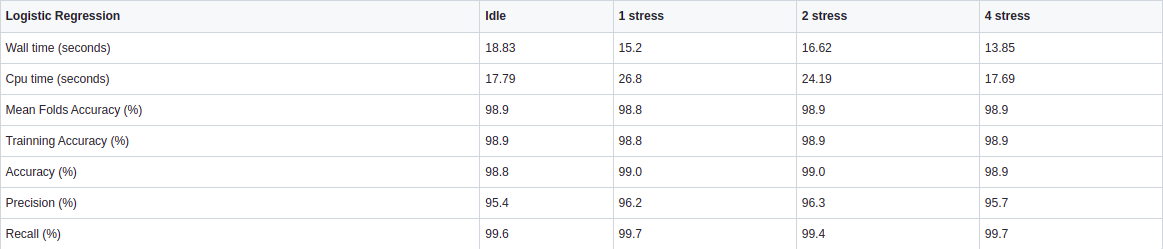
\includegraphics[width=16cm, keepaspectratio]{img/ejemplo_csv.png}
  \caption{Ejemplo de CSV generado con los resultados de cada prueba para el modelo de Regresión Logística.}\label{fig:ejemplo_csv}
\end{figure}

Los nuevos procesos, comentados anteriormente, se crean utilizando la clase de objetos \textit{Popen} de la librería \textit{subprocess}. Nótese que en la función \textit{model} (a diferencia de \textit{start\_stress}) \textit{Popen} tiene añadido al final un \textit{.communicate()} de esta forma se parará la ejecución principal hasta que el proceso de \textit{Popen} termine. Si la función \textit{model} termina y \textit{stress} sigue ejecutando se matará el proceso para poder comandar otro \textit{stress} sin tener que esperar a que se cumpla el tiempo de ejecución que le pasamos como argumento, esto se puede ver en el Código~\ref{lst:funcion_principal_raspberry_test}.

\subsubsection{pc\_test.ipynb}
\label{subsubsec:programa_pruebas_pc}

Este código es prácticamente idéntico al de \texttt{rasp\_test.pynb} salvo pequeñas diferencias. Una de ellas es que en este caso el fichero que generará tras la ejecución de cada modelo tendrá el siguiente formato: \texttt{nombreDataSet\_pcMD.csv}, siendo MD una vez más las siglas del modelo de aprendizaje automático. Al igual que en el caso anterior, se creará una nueva carpeta para guardar todos estos ficheros con el formato: \texttt{nombreDataSet\_pcresults}.

La función principal también utilizará dos bucles anidados para iterar sobre los modelos de aprendizaje con los que se desean experimentar y el número de cores que se van a estresar en cada prueba. En este caso la lista denominada como \textit{num\_cores} variará respecto a la que se declaró en \texttt{raspberry\_test.ipynb} ya que, como se ha comentado antes, en esta ocasión tendremos que saturar otras cantidades de cores. Este programa creará (si es necesario) dos procesos, uno ejecutará stress (cuando se desee estresar alguna CPU) y el otro uno de los modelos que se encuentran dentro de la carpeta \texttt{"Models"}. Todos los ficheros que se utilizan para entrenar los modelos de aprendizaje son los mismos que en la Raspberry Pi salvo el de Random Forest que tiene un fichero específico para el portátil puesto que en este caso, el parámetro \textit{n\_jobs} tendrá que ser igual a ocho, para que el modelo pueda disponer de todos los cores que tiene el portátil. 


\section{Experimentos con datos sintéticos}
\label{sec:exp_dSinteticos}

Como se comentó en el Capítulo~\ref{chap:diseño} en este proyecto se han utilizado varios \textit{datasets} para realizar las pruebas. Dos de estos son ficheros con datos sintéticos, es decir, que no se han generado a través de las medidas de los sensores utilizados en este trabajo. A continuación se explicará en mayor detalle los resultados obtenidos por ambos en cada una de las máquinas.

\subsection{Raspberry Pi}
\label{sub:rasp_sinteticos}

\subsubsection{Resultados Room Occupancy}
\label{subsubsec:occ_raspberry}

Los tiempos de CPU para la ejecución de estos modelos se pueden ver en la Tabla~\ref{tab:times_Occraspberry}\\
\begin{table}[htb]
\begin{adjustbox}{width=\textwidth}
\renewcommand{\arraystretch}{1.5}
\centering
    \begin{tabular}{ @{\extracolsep{5pt}}
    >{\centering\arraybackslash}m{2cm}  
    >{\raggedleft\arraybackslash}m{1.5cm} 
    >{\raggedleft\arraybackslash}m{1.5cm}
    >{\raggedleft\arraybackslash}m{1.5cm}
    >{\raggedleft\arraybackslash}m{1.5cm}
    >{\raggedleft\arraybackslash}m{1.5cm}
    >{\raggedleft\arraybackslash}m{1.5cm}
    >{\raggedleft\arraybackslash}m{1.5cm}
    >{\raggedleft\arraybackslash}m{1.5cm}
    @{}}
    \toprule
    & \multicolumn{8}{c}{\textbf{Nivel de estrés}}\\
    \cline{2-9}
     & \multicolumn{2}{c}{\textbf{Idle}} & \multicolumn{2}{c}{\textbf{2 CPUs}} & \multicolumn{2}{c}{\textbf{4 CPUs}} & \multicolumn{2}{c}{\textbf{8 CPUs}}\\
    \cline{2-3}\cline{4-5}\cline{6-7}\cline{8-9}
    \textbf{Modelo} & CPU time (seg.) & Wall time (seg.) & CPU time (seg.) & Wall time (seg.) & CPU time (seg.) & Wall time (seg.) & CPU time (seg.) & Wall time (seg.)\\
    \midrule
    Regresión Logística & 17,79  & 18,83  & 26,8  & 15,2  & 24,19  & 16,62  & 17,69  & 13,85  \\
    \hline
    SVM & 16,52  & 16,37  & 16,59  & 16,55  & 16,63  & 16,62  & 16,95  & 17,01 \\
    \hline
    Gradient Boosting & 28,61  & 28,74  & 28,4  & 28,38  & 28,3  & 28,31  & 28,51  & 28,66 \\
    \hline
    Random Forest & 59,15  & 24,59  & 52,44  & 26,15  & 48,92  & 30,67  & 49,29  & 34,34 \\
    \hline
    \end{tabular}
\end{adjustbox}
\caption{Resultados de los tiempos de ejecución para el Room Occupancy \textit{dataset} en la Raspberry Pi}
\label{tab:times_Occraspberry}
\end{table}

Los tiempos obtenidos para este \textit{dataset} apenas varían entre los diferentes niveles de saturación (salvo el caso de Random Forest).

Para los modelos de Regresión Logística, Máquinas de Vector Soporte y Gradient Boosting, es normal que apenas varíen sus valores dado que tal y como se explicó en el Capítulo~\ref{chap:diseño} estos tres modelos son \textit{monocores}, es decir, solo pueden ejecutar en una CPU. 

Sin embargo, el modelo de \textit{Random Forest} no terminaba de encajar del todo con lo esperado, que era observar que a medida que aumentase el número de cores estresados también aumentasen los tiempos de CPU. Es por ello que se decidió probar a ejecutar los modelos con un \textit{dataset} con mayor cantidad de datos. De esta forma se podrán observar mejor las razones por las que se obtienen estos tiempos.

Por otra parte, podemos ver como los tiempos de \textit{Wall time} se mantienen prácticamente iguales, exceptuando el caso de Random Forest, a pesar de someter a más carga a la Raspberry Pi. Además para estos modelos, son resultados muy similares a los del \textit{CPU time}, una muestra más de que los procesos no están utilizando la ejecución en paralelo, tal y como se comentó en la sección~\ref{sec:estructura_experimentos}. En cuanto a \textit{Random Forest}, es el único modelo en el que el \textit{Wall time} va incrementando a medida que aumenta el nivel de la prueba, pero aún así devuelve tiempos menores que el \textit{CPU time} indicando que está aprovechando las ventajas de la ejecución paralela. 

En cuanto a la precisión (\textit{Accuracy}) en cada uno de los modelos se obtienen los resultados de la Tabla~\ref{tab:acc_Occraspberry}

\begin{table}[htb]
\renewcommand{\arraystretch}{1.5}
\begin{adjustbox}{width=\textwidth}
\centering
    \begin{tabular}{c  c  c  c  c  c  c}
    \hline
    Modelo & Accuracy CV (\%) & Accuracy trainning (\%) & \multicolumn{4}{c}{Acuracy (\%)} \\
    \cline{4-7}
     &   &   &  Idle & 1 CPU & 2 CPUs & 4 CPUs \\
     \hline
     Regresión Logística & 98,9 & 98,9 & 98,8 & 99,0 & 99,0 & 98,9\\
     SVM & 98,9 & 99,0 & 98,9 & 99,0 & 98,8 & 99,2\\
     Gradient Boosting & 99,0 & 99,4 & 98,9 & 99,1 & 98,7 & 98,9\\
     Random Forest & 99,2 & 100,0 & 99,3 & 99,3 & 99,32 & 99,3\\
    \hline
    \end{tabular}
\end{adjustbox}
\caption{Resultados de la precisión de los modelos para el Room Occupancy \textit{dataset} en Raspberry Pi}
\label{tab:acc_Occraspberry}
\end{table}

Como se puede ver en dicha tabla, en este caso, la diferencia entre la precisión de los datos de entrenamiento y otros datos que no ha visto hasta entonces es muy similar. Por lo tanto los modelos que se están generando son bastante fiables puesto que todos están por encima del $90\%$ de precisión. Y sabemos que no se están sobreajustando puesto que en la columna \texttt{Accuracy CV}, que es la precisión que se obtiene de la validación cruzada, en todos los casos también es superior al $90\%$. Este porcentaje se obtiene de la media de la fila \texttt{Mean Folds Accuracy} de los CSV con los datos generados en cada modelo.

\subsubsection{Resultados $20\%$ KddCup99}
\label{subsubsec:kdd_raspberry}

Los resultados obtenidos para el veinte por ciento del \textit{dataset} de KddCup99 se encuentran en la Tabla~\ref{tab:times_kddraspberry}. En esta ocasión los tiempos de ejecución aumentarán respecto al \textit{dataset} de Room Occupancy puesto que este \textit{dataset} tiene muchas más líneas con las que entrenar (hay más de cuatro millones de líneas de diferencia entre ambos \textit{datasets}).\\
\begin{table}[htb]
\begin{adjustbox}{width=\textwidth}
\renewcommand{\arraystretch}{1.5}
\centering
    \begin{tabular}{ @{\extracolsep{5pt}}
    >{\centering\arraybackslash}m{2cm}  
    >{\raggedleft\arraybackslash}m{1.5cm} 
    >{\raggedleft\arraybackslash}m{1.5cm}
    >{\raggedleft\arraybackslash}m{1.5cm}
    >{\raggedleft\arraybackslash}m{1.5cm}
    >{\raggedleft\arraybackslash}m{1.5cm}
    >{\raggedleft\arraybackslash}m{1.5cm}
    >{\raggedleft\arraybackslash}m{1.5cm}
    >{\raggedleft\arraybackslash}m{1.5cm}
    @{}}
    \toprule
    & \multicolumn{8}{c}{\textbf{Nivel de estrés}}\\
    \cline{2-9}
     & \multicolumn{2}{c}{\textbf{Idle}} & \multicolumn{2}{c}{\textbf{2 CPUs}} & \multicolumn{2}{c}{\textbf{4 CPUs}} & \multicolumn{2}{c}{\textbf{8 CPUs}}\\
    \cline{2-3}\cline{4-5}\cline{6-7}\cline{8-9}
    \textbf{Modelo} & CPU time (seg.) & Wall time (seg.) & CPU time (seg.) & Wall time (seg.) & CPU time (seg.) & Wall time (seg.) & CPU time (seg.) & Wall time (seg.)\\
    \midrule
    Regresión Logística & 447,38  & 142,72  & 506,49  & 191,09  & 422,57  & 223,33  & 387,74  & 211,3  \\
    SVM & 528,55  & 529,74  & 517,1  & 518,07  & 494,24  & 494,31  & 495,47  & 497,24 \\
    Gradient Boosting & 853,97  & 855,97  & 876,88  & 879,19  & 853,42  & 853,49  & 858,95  & 860,68 \\
    Random Forest & 1048,87  & 296,41  & 829,86  & 306,78  & 669,36  & 348,86  & 706,96  & 381,14 \\
    \bottomrule
    \end{tabular}
\end{adjustbox}
\caption{Resultados de los tiempos de ejecución para el $20\%$ Kdd\_cup99 \textit{dataset} en la Raspberry Pi}
\label{tab:times_kddraspberry}
\end{table}

Como se puede observar en la tabla~\ref{tab:times_kddraspberry}, los tiempos de ejecución varían entre los diferentes modelos.

Un vez más, los tiempos de CPU de Regresión Logística, Máquinas de Vector Soporte y Gradient Boosting apenas varían entre los diferentes niveles de estrés, esto se debe a las mismas razones comentadas antes. En el caso de Máquinas de Vector Soporte y Gradient Boosting, \texttt{scikit-learn} no admite \textit{multi-threading}, por lo que a pesar de estresar una, dos o cuatro CPUs siempre devolverán el mismo tiempo puesto que estos modelos solo pueden utilizar un único core para ejecutar.\\
Regresión Logística puede utilizar varios cores si se le indica mediante el parámetro \textit{n\_jobs}. Pero dado que estamos en un problema de clasificación binaria este valor no tendrá ningún efecto al aumentar o disminuir el número de CPUs estresadas como se indicó en el apartado~\ref{subsubsec:lRegression}. 

En cuanto al modelo de Random Forest, para poder entender los tiempos que devuelve, es necesario explicar primero como se comporta la Raspberry Pi cuando varios procesos le piden más recursos de los que tiene y como afecta el parámetro \textit{n\_jobs} a los tiempos de este modelo.

Comencemos explicando como afecta el parámetro \textit{n\_jobs} a los tiempos de ejecución. Como se ha visto anteriormente, Random Forest admite el parámetro \textit{n\_jobs}, que en este caso (a diferencia de Regresión Logística) sí que afecta a como ejecuta el modelo independientemente de si es un problema de clasificación binaria o no. Por lo tanto para poder optimizar el proceso habrá que hacer que el parámetro \textit{n\_jobs} sea igual al número de cores del dispositivo, que en este caso serán cuatro. 

Con este parámetro ajustado hay que tener en cuenta que el tiempo de CPU que obtenemos del comando \textit{time} es la suma de los tiempos que ha necesitado cada uno de los cores utilizados por el proceso para la ejecución. Esta es la razón por la que podemos ver cómo el tiempo en \textit{Idle} es bastante mayor que el resto de casos, puesto que es en esta ocasión donde el programa está pudiendo hacer un uso completo de los cuatro cores, ya que no hay ningún otro proceso que necesite usarlos. Por lo tanto el \textit{CPU time} que tenemos en este nivel es en realidad la suma de los tiempos de ejecución de los cuatro procesadores. El tiempo que ha necesitado cada uno de los cores sería dividir los $1.048,87$ segundos entre 4 con lo que obtendríamos $262$ segundos por core. Sabiendo esto, queda explicado por qué el nivel de \textit{Idle} devuelve un valor tan alto y como esto, que a \textit{priori} puede parecer un poco contradictorio, se ajusta a lo esperado.

Para el resto de casos, dado que ya intervienen otros procesos, habrá que conocer como se comporta la Raspberry Pi ante una mayor demanda de recursos. Lo primero que hay que saber es que el comando \textit{stress} estresará el número de CPUs que se le pasan como argumento siempre y cuando pueda. En el momento en el que tenga que compartir CPU con otros procesos, la Raspberry Pi repartirá los recursos haciendo que \textit{stress} no utilice todas las CPUs que se le ha comandado estresar para que el otro proceso también pueda ejecutar. Por ejemplo, cuando se realiza la prueba de nivel alto de carga al modelo de Máquinas de Vector Soporte, si se comprueban los valores de CPU que utiliza cada uno de los procesos (por medio del comando \textit{htop} de Linux), aunque se puede ver que \textit{stress} tiene cuatro procesos, la suma de lo que utiliza la CPU cada uno de ellos será igual a un total de tres cores más o menos, es decir utilizan un $300\%$ de los recursos. Mientras que el proceso del modelo utiliza una CPU, un $100\%$. Siendo el valor total de los recursos de los que dispone la Raspberry Pi igual a $400\%$, un $100\%$ para cada uno de los cores de la Raspberry Pi.

Otro ejemplo de esto puede ser el caso en el que se ejecuta el modelo de Random Forest, teniendo el parámetro de \textit{n\_jobs} igual a cuatro para utilizar todos los cores disponibles, a la vez que \textit{stress} para estresar las cuatro CPUs. Si observamos mediante el comando \textit{htop} los procesos, se podrá ver como se distribuyen los cores para que puedan ejecutar a la vez tanto los procesos de \textit{stress} como los del modelo de aprendizaje. Por lo tanto \textit{stress} utilizará en total dos CPUs y Random Forest hará lo mismo, pese a que a ambos se les indicó que utilizasen todas las CPUs de la Raspberry Pi. Este ejemplo se puede ver en la Figura~\ref{figura:stress_rForest}, siendo la CPU total que utiliza Random Forest la que se indica en el primer proceso que muestra \textit{htop} en la imagen. Al sumar el resto de procesos de RF su valor de CPU es igual al del primer proceso.

 \begin{figure}[htb]
    \centering
    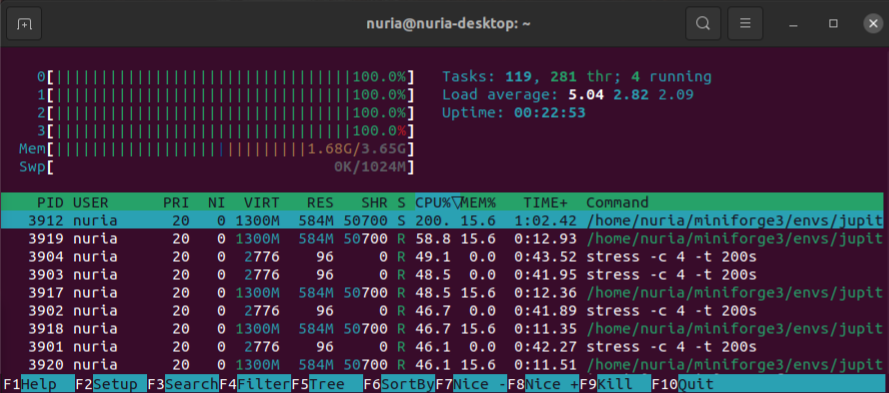
\includegraphics[ width=16cm, keepaspectratio]{img/rForest_stress2.png}
    \caption{Porcentaje de CPU utilizada por los procesos al ejecutar Random Forest con cuatro CPUs estresadas.}
    \label{figura:stress_rForest}
 \end{figure}

En la Figura~\ref{figura:stress_rForest} vemos que el primer proceso de RF está consumiendo el $200\%$ de CPU. Mientras que si sumamos los porcentajes de los cuatro procesos de \textit{stress} obtendremos que se están consumiendo en total un $190\%$, prácticamente un $200\%$. Por lo que, a pesar de lo que se ha comandado, la Raspberry Pi dividirá los recursos para que ambos procesos puedan usar lo máximo posible.

Sabiendo esto, los niveles de prueba medio y alto para el modelo de Random Forest obtienen prácticamente los mismos tiempos puesto que al tratar de ejecutar a la vez tanto el proceso de \textit{stress} como el del modelo, se están pidiendo usar más cores de los que hay. En consecuencia la Raspberry Pi tendrá que dividir los recursos de los que dispone equitativamente entre ambos procesos. Por lo que en el fondo \textit{stress} estará estresando el mismo número de CPUs tanto en el nivel medio como en el alto. Y al proceso del modelo le sucederá lo mismo, utilizará el mismo número de procesadores tanto en un caso como en el otro. En el nivel intermedio, donde se estresan dos cores, el modelo no podrá utilizar las cuatro CPUs que se le indican con \textit{n\_jobs} puesto que estaría superando el número de cores que posee la Raspberry Pi. De modo que la Raspberry Pi dividirá los recursos haciendo que \textit{stress} pueda ejecutar en dos cores, y por lo tanto el modelo de aprendizaje dispondrá únicamente de las otras dos CPUs para su ejecución. Mientras que en el nivel más alto de carga la Raspberry Pi dividirá las cuatro CPUs para darle la mitad de ellas a la ejecución de \textit{stress} y la otra mitad al modelo, haciendo que ambas utilicen el máximo de procesadores posibles. Esta es la explicación para los tiempos del nivel medio y alto. 

En el nivel bajo encontraremos que el modelo solo puede estar usando tres cores para dejarle el cuarto a \textit{stress}. Como hemos visto el tiempo de CPU es el tiempo total que han usado los tres procesadores, luego por cada core el proceso ha tardado unos $276$ seg (el resultado de dividir $829,86$ seg entre los tres cores). Por lo tanto el tiempo aumenta un poco del estado respecto al nivel \textit{Idle}.

Algo destacable de los resultados obtenidos en este \textit{dataset} (a diferencia del de Room Occupancy) es que salvo en el nivel de \textit{Idle}, el modelo de Gradient Boosting llega a ser más lento que el modelo de Random Forest, modelo que en el anterior \textit{dataset} era con diferencia el que tardaba más tiempo de todos.

En cuanto al \textit{Wall time} obtenido vemos que por un lado Random Forest aumenta su tiempo a medida que aumenta la carga computacional, igual que lo hacía en el anterior \textit{dataset}, pero siendo en cada caso los tiempos menores que el \textit{CPU time}. Mientras que tanto el modelo de SVM como de GB se mantienen más o menos constantes e iguales al \textit{CPU time}, indicando que no se están ejecutando procesos en paralelo. Y por último, Regresión Logística es el que más varía entre las diferentes pruebas, siendo siempre el \textit{Wall time} menor que el \textit{CPU time}.

Otro aspecto de las ejecuciones en la Raspberry Pi que será relevante más adelante, es la frecuencia a la que ejecutan los cores. Utilizando el comando \textit{lscpu} de Linux, se puede obtener información relevante sobre los cores como por ejemplo la frecuencia máxima y mínima a la que pueden ejecutar, que en el caso de la Raspberry Pi la mínima será igual a $600MHz$ y la máxima $1.500MHz$. 

Para saber la frecuencia de cada uno de los cores en tiempo real se puede ejecutar el comando:\\

\begin{lstlisting}[language=bash, showstringspaces=false]
   $ watch -n.1 "
   sudo cat /sys/devices/system/cpu/cpu0/cpufreq/cpuinfo_cur_freq && 
   sudo cat /sys/devices/system/cpu/cpu1/cpufreq/cpuinfo_cur_freq && 
   sudo cat /sys/devices/system/cpu/cpu2/cpufreq/cpuinfo_cur_freq && 
   sudo cat /sys/devices/system/cpu/cpu3/cpufreq/cpuinfo_cur_freq"
\end{lstlisting}

Mostrará las frecuencias de ejecución de los cores cada $0,1$ segundos. Si utilizamos dicho comando para ver las frecuencias cuando la Raspberry Pi está tanto \textit{Idle} como estresada podremos ver que todas las CPUs están sobre los $1.500MHz$. Por lo tanto todos los cores siempre están ejecutando a la máxima velocidad que pueden.

Por otra parte los resultados de precisión para este \textit{dataset} se pueden observar en la Tabla~\ref{tab:acc_Kddraspberry}. Al igual que en el caso del Room Occupancy Dataset se obtienen muy buenos resultados, estando prácticamente todos cerca del $100\%$ de \textit{Accurancy}, y sabiendo que no se están sobreajustando puesto que la precisión de la validación cruzada también es prácticamente el $100\%$ en todos los casos.

\begin{table}[htb]
\renewcommand{\arraystretch}{1.5}
\begin{adjustbox}{width=\textwidth}
\centering
    \begin{tabular}{c  c  c  c  c  c  c}
    \hline
    Modelo & Accuracy CV (\%) & Accuracy trainning (\%) & \multicolumn{4}{c}{Acuracy (\%)} \\
    \cline{4-7}
     &  &   &  Idle & 1 CPU & 2 CPUs & 4 CPUs \\
     \hline
     Regresión Logística & 99,4 & 99,4 & 99,4 & 99,4 & 99,4 & 99,4\\
     SVM & 99,9 & 99,9 & 99,8 & 99,9 & 98,8 & 99,8\\
     Gradient Boosting & 99,9 & 100,0 & 96,4 & 98,8 & 99,4 & 73,0\\
     Random Forest & 100,0 & 100,0 & 97,5 & 97,9 & 96,9 & 98,6\\
    \hline
    \end{tabular}
\end{adjustbox}
\caption{Resultados de la precisión de los modelos para el $20\%$ Kdd\_cup99 \textit{dataset} en Raspberry Pi}
\label{tab:acc_Kddraspberry}
\end{table}

Por último, añadir que con este set de datos se hicieron varias pruebas con distintas cantidades (porcentajes) de datos procedentes del \textit{dataset} total, obteniendo en todos ellos los mismos comportamientos. Lo único que variaba eran los tiempos totales de ejecución que para porcentajes más pequeños decrementaban y para mayores aumentaban. La única diferencia notable que se encontró al realizar las pruebas para \textit{datasets} de porcentajes pequeños (que contenían menos del $10\%$ de los datos totales) era que el modelo de Gradient Boosting y Regresión Logística tenían prácticamente los mismos tiempos de ejecución en los diferentes niveles de saturación.

\subsection{Portátil}
\label{subsec:pc_sinteticos}

\subsubsection{Resultados Room Occupancy}
\label{subsubsec:occ_pc}

Los tiempos de ejecución que empleó el portátil para entrenar los diferentes modelos con este \textit{dataset} se encuentran en la Tabla~\ref{tab:times_Occpc}
\begin{table}[htb]
\begin{adjustbox}{width=\textwidth}
\renewcommand{\arraystretch}{1.5}
\centering
    \begin{tabular}{ @{\extracolsep{5pt}}
    >{\centering\arraybackslash}m{2cm}  
    >{\raggedleft\arraybackslash}m{1.5cm} 
    >{\raggedleft\arraybackslash}m{1.5cm}
    >{\raggedleft\arraybackslash}m{1.5cm}
    >{\raggedleft\arraybackslash}m{1.5cm}
    >{\raggedleft\arraybackslash}m{1.5cm}
    >{\raggedleft\arraybackslash}m{1.5cm}
    >{\raggedleft\arraybackslash}m{1.5cm}
    >{\raggedleft\arraybackslash}m{1.5cm}
    @{}}
    \toprule
    & \multicolumn{8}{c}{\textbf{Nivel de estrés}}\\
    \cline{2-9}
     & \multicolumn{2}{c}{\textbf{Idle}} & \multicolumn{2}{c}{\textbf{2 CPUs}} & \multicolumn{2}{c}{\textbf{4 CPUs}} & \multicolumn{2}{c}{\textbf{8 CPUs}}\\
    \cline{2-3}\cline{4-5}\cline{6-7}\cline{8-9}
    \textbf{Modelo} & CPU time (seg.) & Wall time (seg.) & CPU time (seg.) & Wall time (seg.) & CPU time (seg.) & Wall time (seg.) & CPU time (seg.) & Wall time (seg.)\\
    \midrule
    Regresión Logística & 2,31  & 1,9  & 2,56  & 1,615  & 2,63  & 1,71  & 5,53  & 3,5  \\
    SVM & 3,29  & 3,3  & 3,65  & 3,65  & 6,16  & 6,17  & 6,24  & 7,52 \\
    Gradient Boosting & 7,5  & 7,54  & 8,13  & 8,14  & 10,44  & 10,45  & 17,16  & 21,47 \\
    Random Forest & 18,22  & 3,97  & 16,43  & 4,55  & 16,61  & 6,16  & 21,64  & 10,83 \\
    \bottomrule
    \end{tabular}
\end{adjustbox}
\caption{Resultados de los tiempos de ejecución para el Room Occupancy \textit{dataset} en el portátil}
\label{tab:times_Occpc}
\end{table}

En esta ocasión, a diferencia del comportamiento de la Raspberry Pi los tiempos de CPU van aumentando con las diferentes pruebas, aun cuando los tres primeros modelos solo pueden ejecutar en una CPU y por lo tanto no deberían de afectarles que hubiese más de un core estresado. Sin embargo, este incremento en los tiempos se puede deber a la frecuencia con la que ejecutan las CPUs. En el portátil la frecuencia máxima a la que pueden ejecutar los cores es de $3.600MHz$ mientras que la mínima son $400MHz$. 

Ejecutando el siguiente comando: 

\begin{lstlisting}[language=bash, showstringspaces=false]
  $ watch -n.1 "grep \"^[c]pu MHz\" /proc/cpuinfo"
\end{lstlisting}

Se puede ver la frecuencia de ejecución de todos los cores cada $0,1$ segundos. En esta ocasión, al observar estas velocidades cuando se ejecutaban los algoritmos de aprendizaje automático se podía ver una variación en los valores dependiendo del nivel de estrés que se estuviese ejecutando, a diferencia de lo que ocurría en la Raspberry Pi que se mantenía siempre a la máxima frecuencia. Esto explicaría porque en el caso del portátil los tiempos incrementan según aumentan el número de cores estresados. 

Por otra parte, el \textit{Wall time} tiene un comportamiento similar al de \textit{CPU time} aumentando a medida que se incrementa el nivel de carga computacional en todos los modelos. Sin embargo, en el caso de SVM y GB se puede ver que la diferencia entre el \textit{CPU time} y \textit{Wall time} es muy pequeña, por tanto podemos seguir afirmando que se está usando un solo core aunque todos los tiempos aumenten conforme más CPUs se estresan.

Veamos a continuación cual es el \textit{Accuracy} que consiguen los modelos con este \textit{dataset} en esta máquina.\\
\begin{table}[htb]
\renewcommand{\arraystretch}{1.5}
\begin{adjustbox}{width=\textwidth}
\centering
    \begin{tabular}{c  c  c  c  c  c  c}
    \hline
    Modelo & Accuracy CV (\%) & Accuracy trainning (\%) & \multicolumn{4}{c}{Acuracy (\%)} \\
    \cline{4-7}
      &  &   &  Idle & 2 CPUs & 4 CPUs & 8 CPUs \\
     \hline
     Regresión Logística & 98,9 & 99,0 & 98,9 & 98,9 & 98,7 & 99,0\\
     SVM & 99,0 & 99,0 & 98,9 & 98,8 & 99,0 & 98,8\\
     Gradient Boosting & 99,0 & 99,3 & 99,0 & 98,9 & 98,8 & 99,0\\
     Random Forest & 99,2 & 100,0 & 99,2 & 99,3 & 99,1 & 99,2\\
    \hline
    \end{tabular}
\end{adjustbox}
\caption{Resultados de la precisión de los modelos para el Room Occupancy \textit{dataset} en el portátil}
\label{tab:acc_Occpc}
\end{table}

En la Tabla~\ref{tab:acc_Occpc} se puede ver que en este caso también se consiguen unos modelos de gran precisión tanto en la validación cruzada, como con los datos de entrenamiento además de en cada una de las diferentes pruebas.

\subsubsection{Resultados $20\%$ Kdd\_cup99}
\label{subsubsec:kdd_pc}

Los resultados de la ejecución del comando \textit{stress} conforme a estos niveles se pueden observar en la tabla~\ref{tab:times_kddportatil}. Como se puede apreciar los tiempos que se obtienen en el portátil disminuyen bastante con respecto a los que conseguía la Raspberry Pi.

\begin{table}[htb]
\begin{adjustbox}{width=\textwidth}
\renewcommand{\arraystretch}{1.5}
\centering
    \begin{tabular}{ @{\extracolsep{5pt}}
    >{\centering\arraybackslash}m{2cm}  
    >{\raggedleft\arraybackslash}m{1.5cm} 
    >{\raggedleft\arraybackslash}m{1.5cm}
    >{\raggedleft\arraybackslash}m{1.5cm}
    >{\raggedleft\arraybackslash}m{1.5cm}
    >{\raggedleft\arraybackslash}m{1.5cm}
    >{\raggedleft\arraybackslash}m{1.5cm}
    >{\raggedleft\arraybackslash}m{1.5cm}
    >{\raggedleft\arraybackslash}m{1.5cm}
    @{}}
    \toprule
    & \multicolumn{8}{c}{\textbf{Nivel de estrés}}\\
    \cline{2-9}
     & \multicolumn{2}{c}{\textbf{Idle}} & \multicolumn{2}{c}{\textbf{2 CPUs}} & \multicolumn{2}{c}{\textbf{4 CPUs}} & \multicolumn{2}{c}{\textbf{8 CPUs}}\\
    \cline{2-3}\cline{4-5}\cline{6-7}\cline{8-9}
    \textbf{Modelo} & CPU time (seg.) & Wall time (seg.) & CPU time (seg.) & Wall time (seg.) & CPU time (seg.) & Wall time (seg.) & CPU time (seg.) & Wall time (seg.)\\
    \midrule
    Regresión Logística & 67,95  & 20,28  & 99,58  & 29,96  & 126,63  & 44,05  & 168,25  & 77,76  \\
    SVM & 114,81  & 116,45  & 166,42  & 168,05  & 317,07  & 318,72  & 327,69  & 365,5 \\
    Gradient Boosting & 176,09  & 177,74  & 232,99  & 234,63  & 268,3  & 270,03  & 390,09  & 429,31 \\
    Random Forest & 392,73  & 55,88  & 327,2  & 59,44  & 291,76  & 69,48  & 256,92  & 81,99 \\
    \bottomrule
    \end{tabular}
\end{adjustbox}
\caption{Resultados de los tiempos de ejecución para el $20\%$ Kdd\_cup99 \textit{dataset} en el portátil.}
\label{tab:times_kddportatil}
\end{table}

Según esta tabla, Random Forest es el modelo que más tiempo de CPU tarda cuando la máquina se encuentra en estado \textit{Idle} y se mantienen el resto de pruebas sobre los $300$ segundos de ejecución. Esto se debe a las mismas razones dadas en la sección~\ref{subsubsec:kdd_raspberry}. El hecho de que, en los modelos \textit{monocore}, los tiempos aumenten al aumentar el nivel de estrés, se debe a las mismas razones comentadas en la ejecución del \textit{dataset} de Room Occupancy en el portátil~\ref{subsubsec:occ_pc}.

Y al igual que en el anterior \textit{dataset}, el \textit{Wall time} aumenta conforme más cores se estresan. Manteniendo es todos los casos las mismas relaciones con el \textit{CPU time}.

Respecto a la precisión de los modelos generados podemos ver los resultados en la Tabla~\ref{tab:acc_Kddpc}. Que al igual que los valores obtenidos en el anterior \textit{dataset} los datos no se sobreajustan y se están consiguiendo resultados de gran precisión en todas las pruebas.\\
\begin{table}[htb]
\renewcommand{\arraystretch}{1.5}
\begin{adjustbox}{width=\textwidth}
\centering
    \begin{tabular}{c  c  c  c  c  c  c}
    \hline
    Modelo & Accuracy CV (\%) & Accuracy trainning (\%) & \multicolumn{4}{c}{Acuracy (\%)} \\
    \cline{4-7}
     &  &   &  Idle & 2 CPUs & 4 CPUs & 8 CPUs \\
     \hline
     Regresión Logística & 99,4 & 99,4 & 99,4 & 99,4 & 99,4 & 99,4\\
     SVM & 99,9 & 99,9 & 99,9 & 99,8 & 99,8 & 99,9\\
     Gradient Boosting & 99,9 & 100,0 & 96,4 & 96,5 & 99,3 & 99,3 \\
     Random Forest & 100,0 & 100,0 & 99,7 & 97,4 & 99,7 & 96,8\\
    \hline
    \end{tabular}
\end{adjustbox}
\caption{Resultados de la precisión de los modelos para el $20$\% Kdd\_cup99 \textit{dataset} en el portátil}
\label{tab:acc_Kddpc}
\end{table}

\subsection{Conclusiones datos sintéticos}
\label{subsec:conclusion_sinteticos}

Tras haber observado los resultados obtenidos en la ejecución de cada uno de los modelos en diferentes situaciones de estrés en ambos dispositivos con los dos \textit{datasets}, se ha podido comprobar qué a pesar de la menor capacidad de la Raspberry Pi, esta consigue un comportamiento bastante bueno.

Donde más se nota la falta de recursos de la Raspberry Pi es en los tiempos de ejecución. Para los mismos modelos y los mismos datos, tarda más en ejecutar la Raspberry Pi que el portátil. En la Figura~\ref{fig:per_occupancy} se muestra utilizando porcentajes cuánto de lenta es la Raspberry Pi respecto al portátil en cada uno de los niveles de estrés para el Room Occupancy Dataset, utilizando los tiempos de CPU.

\begin{figure}[htb]
  \centering
  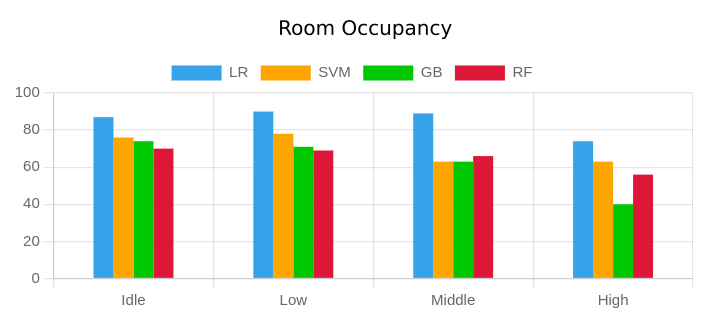
\includegraphics[width=14cm, keepaspectratio]{img/per_occupancy.png}
  \caption{Porcentaje de lentitud de la Raspberry Pi respecto al portátil para Room Occupancy.}
  \label{fig:per_occupancy}
\end{figure}

En dicha figura podemos ver como a medida que el nivel de saturación aumenta (eje x) es menor el porcentaje de lentitud, con lo que cada vez es menor la diferencia entre los tiempos de ejecución de la Raspberry Pi y del portátil. Siendo el modelo de RL en el que mayor diferencia hay entre ambas máquinas. Aunque este modelo es el que menos tarda en ejecutar en el portátil no sucede siempre lo mismo en la Raspberry Pi lo que hace que se termine convirtiendo en el modelo que peor se comporta en la Raspberry Pi al compararlo con el portátil, siendo en media un $85\%$ más lento en la Raspberry Pi que en el portátil.

Mientras que en el caso de SVM la Raspberry Pi es $70\%$ (en media) más lenta. Además observando la Tabla~\ref{tab:times_Occraspberry} podemos ver que es el modelo que más rápido entrena en todos los niveles de estrés, a pesar de ser \textit{monocore} obtiene el mejor rendimiento de todos. Mientras que en el portátil es el segundo modelo con mejores tiempos en todos los casos, después de RL (Tabla \ref{tab:times_Occpc}).

El modelo de Gradient Boosting es el único que consigue estar en algún momento por debajo del $50\%$ de lentitud. Cuando ambas máquinas están con todos los cores estresados, GB es solo un $40\%$ más lento en la Raspberry Pi que en el portátil. El porcentaje medio de lentitud de este modelo es de $62\%$, es decir, que solo es un $62\%$ más lento en la Raspberry Pi que en el portátil, obteniendo la mejor relación de tiempos entre ambas máquinas de todos los modelos, a pesar de que en ninguna de ellas sea de los modelos más rápidos.

Por último, el porcentaje medio de lentitud para el modelo de Random Forest es igual a el $65\%$. En la Tabla~\ref{tab:times_Occraspberry} como en la Tabla~\ref{tab:times_Occpc} se puede ver que, con diferencia, este es el modelo más lento en ambas máquinas. Sin embargo, hay que recordar que los tiempos de CPU en estos casos, son el resultado de la suma de los tiempos en cada uno de los cores. Por lo tanto, si dividimos esos tiempos entre el número de CPUs que se han utilizado en cada nivel, la diferencia de tiempos no es tan grande respecto al resto de modelos pero sigue tardando un poco más. En el nivel de \textit{Idle}, en el caso de la Raspberry Pi, el tiempo empleado por cada CPU es de $14,78$ seg, mientras que en el portátil serían $2,27$ seg.

De la misma forma, en la Figura~\ref{fig:per_kdd} se muestra estos mismos porcentajes de lentitud pero esta vez para el caso del \textit{dataset} KddCup99.

\begin{figure}[htb]
  \centering
  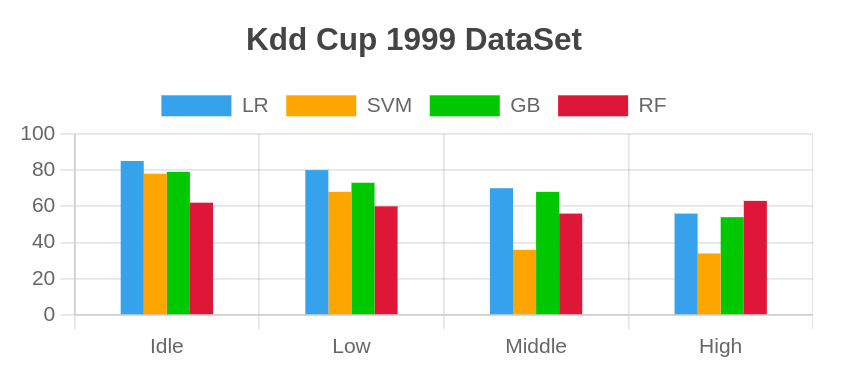
\includegraphics[width=14cm, keepaspectratio]{img/per_kdd.png}
  \caption{Porcentaje de lentitud de la Raspberry Pi respecto al portátil para KddCup99.}
  \label{fig:per_kdd}
\end{figure}

Al igual que antes los porcentajes van decrementando a medida que más CPUs están estresadas. En este caso sigue siendo el modelo de RL el que peor comportamiento realiza en comparación con el portátil, obteniendo un porcentaje de lentitud medio del $72,75\%$. Pese a que en este caso es el modelo más rápido para todos los niveles tanto en la Raspberry Pi como en el portátil (Tabla~\ref{tab:times_kddraspberry} y Tabla~\ref{tab:times_kddportatil}), sin embargo la diferencia de tiempos entre ambas máquinas es muy grande, de unos $300$ segundos, lo que hace que este porcentaje sea tan alto.

Por otra parte, esta vez es el modelo de SVM el que en la Raspberry Pi es un $54\%$ de media más lento que el portátil, consiguiendo que su porcentaje de lentitud sea menor del $40\%$ para los dos últimos niveles. Por lo que, para este \textit{dataset}, es el modelo en el que los tiempos de ejecución son más similares en ambas máquinas, siendo en ambos casos el segundo modelo más rápido para todos los niveles de estrés.

Gradient Boosting sigue siendo el segundo más lento de todos, consiguiendo ser en los tres últimos niveles de estrés de la Raspberry Pi incluso más lento que Random Forest, y en el portátil es el más lento para los últimos dos niveles (Tabla~\ref{tab:times_kddraspberry} y Tabla~\ref{tab:times_kddportatil}). En media, este modelo actúa un $70,75\%$ más lento en la Raspberry Pi que en el portátil. Por lo tanto, Random Forest no siempre es el modelo más lento para este \textit{dataset}, teniendo un porcentaje de lentitud del $60\%$. 

Una de las razones por las que todos los modelos en la Raspberry Pi sean más lentos que en el portátil es debido a las frecuencias con las que ejecutan ambas máquinas. Observándolas vemos que la máxima velocidad a la que pueden ir los cores en la Raspberry Pi es a $1.500MHz$ mientras que el portátil tiene su máximo en $3.600MHz$, más del doble que la Raspberry Pi. Esto permite que los procesos en el portátil puedan terminar antes que en la Raspberry Pi siendo uno de los factores por los que esta máquina puede ser más lenta que el portátil, ya que los cores pueden ir a mayor velocidad.

Otro factor que puede estar ayudando a que la diferencia de tiempos entre ambas máquinas sea mayor es, como cabe esperar, debido a que la Raspberry Pi dispone de la mitad de cores que posee el portátil.

Ambos aspectos son los que pueden hacer notoria la gran diferencia de tiempos de ejecución en ambas máquinas.

Sin embargo, a parte de la diferencia de los tiempos, todos los modelos tanto entrenando en la Raspberry Pi como en el portátil alcanzaban un \textit{Accuracy}, \textit{Precision} y \textit{Recall} mayor al $90\%$ prácticamente siempre en todos los casos.

\section{Experimentos con los datos capturados por sensores}
\label{sec:exp_dSensados}

Tal y como se comentó en el apartado~\ref{sec:mi_dataSet} se generó un \textit{dataset} mediante los datos proporcionados por los sensores. Este set de datos se denomina como \texttt{occup\_detec\_2h\_Clean.csv}, en total contiene $9.745$ líneas de datos que equivalen a unas dos horas y cuarenta minutos de recolección de datos.

\subsection{Raspberry Pi}
\label{subsec:rasp_sensados}

Los resultados de los tiempos de ejecución para el \textit{dataset} generado por medio de los datos, obtenidos de los sensores, se pueden ver en la Tabla~\ref{tab:times_sensrasp}.\\
\begin{table}[htb]
\begin{adjustbox}{width=\textwidth}
\renewcommand{\arraystretch}{1.5}
\centering
    \begin{tabular}{ @{\extracolsep{5pt}}
    >{\centering\arraybackslash}m{2cm}  
    >{\raggedleft\arraybackslash}m{1.5cm} 
    >{\raggedleft\arraybackslash}m{1.5cm}
    >{\raggedleft\arraybackslash}m{1.5cm}
    >{\raggedleft\arraybackslash}m{1.5cm}
    >{\raggedleft\arraybackslash}m{1.5cm}
    >{\raggedleft\arraybackslash}m{1.5cm}
    >{\raggedleft\arraybackslash}m{1.5cm}
    >{\raggedleft\arraybackslash}m{1.5cm}
    @{}}
    \toprule
    & \multicolumn{8}{c}{\textbf{Nivel de estrés}}\\
    \cline{2-9}
     & \multicolumn{2}{c}{\textbf{Idle}} & \multicolumn{2}{c}{\textbf{2 CPUs}} & \multicolumn{2}{c}{\textbf{4 CPUs}} & \multicolumn{2}{c}{\textbf{8 CPUs}}\\
    \cline{2-3}\cline{4-5}\cline{6-7}\cline{8-9}
    \textbf{Modelo} & CPU time (seg.) & Wall time (seg.) & CPU time (seg.) & Wall time (seg.) & CPU time (seg.) & Wall time (seg.) & CPU time (seg.) & Wall time (seg.)\\
    \midrule
    Regresión Logística & 10,73  & 9,51  & 19,39  & 12,52  & 18,73  & 13,77  & 17,4  & 13,38  \\
    
    SVM & 10,48  & 10,35  & 10,32  & 10,24  & 10,26  & 10,21  & 10,27  & 10,44 \\
   
    Gradient Boosting & 17,28  & 17,17  & 17,15  & 17,1  & 17,11  & 17,08  & 17,07  & 17,14 \\
   
    Random Forest & 42,58  & 20,21  & 38,37  & 21,2  & 35,41  & 23,93  & 36,78  & 27,68 \\
    \bottomrule
    \end{tabular}
\end{adjustbox}
\caption{Resultados de los tiempos de ejecución para el \textit{dataset} de Sensores Raspberry Pi en la Raspberry Pi.}
\label{tab:times_sensrasp}
\end{table}

Como se puede observar, se mantiene un comportamiento tanto en los tiempos de CPU como en \textit{Wall time} bastante similar a lo visto en los anteriores \textit{datasets} ejecutados en la Raspberry Pi. Por un lado SVM y GB se mantiene prácticamente iguales en todas las pruebas. Y en RF en el nivel \textit{Idle} es cuando más tarda el \textit{CPU time}, mientras que el \textit{Wall time} aumenta manteniéndose siempre por debajo del \textit{CPU time}.

Por otro lado, la precisión obtenida por medio de este \textit{dataset} se encuentra en la Tabla~\ref{tab:acc_sensrasp}.\\
\begin{table}[htb]
\renewcommand{\arraystretch}{1.5}
\begin{adjustbox}{width=\textwidth}
\centering
    \begin{tabular}{c  c  c  c  c  c  c}
    \hline
    Modelo & Accuracy CV (\%) & Accuracy trainning (\%) & \multicolumn{4}{c}{Acuracy (\%)} \\
    \cline{4-7}
     &  &   &  Idle & 1 CPU & 2 CPUs & 4 CPUs \\
     \hline
     Regresión Logística & 98,9 & 99,0 & 99,2 & 99,1 & 99,2 & 99,0\\
     SVM & 99,5 & 99,6 & 99,5 & 99,5 & 98,6 & 98,5\\
     Gradient Boosting & 99,9 & 100,0 & 99,9 & 99,8 & 99,5 & 98,9\\
     Random Forest & 99,9 & 100,0 & 99,8 & 99,9 & 99,7 & 99,7\\
    \hline
    \end{tabular}
\end{adjustbox}
\caption{Resultados de la precisión de los modelos para el \textit{dataset} Sensores Raspberry Pi en la Raspberry Pi.}
\label{tab:acc_sensrasp}
\end{table}

A pesar de ser el \textit{dataset} con el menor número de muestras de todos los que se han visto en este proyecto, la precisión que alcanzan los modelos sigue siendo muy alta.

\subsection{Portátil}
\label{subsec:pc_sensados}

Los resultados de los tiempos de ejecución para el \textit{dataset} generado por medio de los datos obtenidos de los sensores se pueden ver en la Tabla~\ref{tab:times_senspc}.
\begin{table}[htb]
\begin{adjustbox}{width=\textwidth}
\renewcommand{\arraystretch}{1.5}
% \newcolumntype{a}{>{\columncolor{myLightGray}}c}
\centering
    \begin{tabular}{ @{\extracolsep{5pt}}
    >{\centering\arraybackslash}m{2cm}  
    >{\raggedleft\arraybackslash}m{1.5cm} 
    >{\raggedleft\arraybackslash}m{1.5cm}
    >{\raggedleft\arraybackslash}m{1.5cm}
    >{\raggedleft\arraybackslash}m{1.5cm}
    >{\raggedleft\arraybackslash}m{1.5cm}
    >{\raggedleft\arraybackslash}m{1.5cm}
    >{\raggedleft\arraybackslash}m{1.5cm}
    >{\raggedleft\arraybackslash}m{1.5cm}
    @{}}
    \toprule
    & \multicolumn{8}{c}{\textbf{Nivel de estrés}}\\
    \cline{2-9}
     & \multicolumn{2}{c}{\textbf{Idle}} & \multicolumn{2}{c}{\textbf{2 CPUs}} & \multicolumn{2}{c}{\textbf{4 CPUs}} & \multicolumn{2}{c}{\textbf{8 CPUs}}\\%[2ex]
    \cline{2-3}\cline{4-5}\cline{6-7}\cline{8-9}
    \textbf{Modelo} & CPU time (seg.) & Wall time (seg.) & CPU time (seg.) & Wall time (seg.) & CPU time (seg.) & Wall time (seg.) & CPU time (seg.) & Wall time (seg.)\\%[2ex]
    \midrule
    Regresión Logística & 2,0  & 1,36  & 2,27  & 1,55  & 2,96  & 2,24  & 3,27  & 2,81  \\%[2ex]
    
    SVM & 1,65  & 1,66  & 1,77  & 1,78  & 2,71  & 2,72  & 2,8  & 3,23 \\%[2ex]
    
    Gradient Boosting & 3,67  & 3,67  & 4,12  & 4,13  & 4,28  & 4,29  & 6,18  & 7,18 \\%[2ex]
    
    Random Forest & 13,29  & 3,35  & 12,28  & 3,87  & 11,82  & 4,57  & 13,29  & 8,39 \\%[2ex]
    \bottomrule
    \end{tabular}
\end{adjustbox}
\caption{Resultados de los tiempos de ejecución para el \textit{dataset} Sensores Raspberry Pi en el portátil.}
\label{tab:times_senspc}
\end{table}

Una vez más es muy similar al comportamiento que realizaban los tiempos en los anteriores \textit{datasets}. Incrementan a medida que aumentan el número de procesadores estresados.

Mientras que la precisión obtenida por medio de este \textit{dataset} se encuentra en la Tabla~\ref{tab:acc_senspc}.\\
\begin{table}[htb]
\renewcommand{\arraystretch}{1.5}
\begin{adjustbox}{width=\textwidth}
\centering
    \begin{tabular}{c  c  c  c  c  c  c}
    \toprule
    Modelo & Accuracy CV (\%) & Accuracy trainning (\%) & \multicolumn{4}{c}{Acuracy (\%)} \\
    \cline{4-7}
     &  &   &  Idle & 2 CPUs & 4 CPUs & 8 CPUs \\
     \midrule
     Regresión Logística & 99,0 & 99,0 & 99,0 & 99,0 & 99,1 & 99,8\\
     SVM & 99,5 & 99,5 & 99,7 & 99,5 & 98,6 & 98,6\\
     Gradient Boosting & 99,9 & 100,0 & 99,7 & 99,9 & 99,5 & 99,8\\
     Random Forest & 99,9 & 100,0 & 99,5 & 99,8 & 99,7 & 99,5\\
    \bottomrule
    \end{tabular}
\end{adjustbox}
\caption{Resultados de la precisión de los modelos para el \textit{dataset} Sensores Raspberry Pi en el portátil.}
\label{tab:acc_senspc}
\end{table}

Obteniendo como cabía esperar resultados de precisión muy buenos, y sabiendo que en ningún momento se ha sobreajustado ningún modelo gracias a el porcentaje de validación cruzada tan elevado que se consigue en todos los casos.

\subsection{Conclusiones de los datos capturados por los sensores}
\label{subsec:conclusiones_sensados}

Con los resultados obtenidos podemos llegar a las mismas conclusiones que en el caso de los datos sintéticos, a pesar de las limitaciones que tiene la Raspberry Pi esta es capaz de llevar a cabo perfectamente las tareas encomendadas.

En este caso los porcentajes de lentitud de la Raspberry Pi respecto del portátil (utilizando los tiempos de CPU) se pueden ver en la Figura~\ref{fig:per_Mi}.

\begin{figure}[htb]
  \centering
  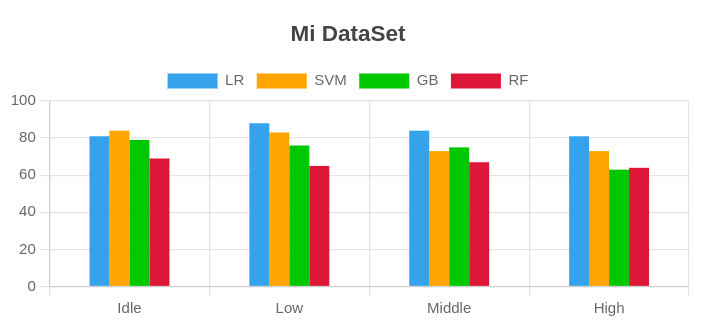
\includegraphics[width=14cm, keepaspectratio]{img/per_mi.png}
  \caption{Porcentaje de lentitud de la Raspberry Pi respecto al portátil para el \textit{dataset} Sensores Raspberry Pi}
  \label{fig:per_Mi}
\end{figure}

En esta ocasión, salvo en el caso \textit{Idle}, sigue siendo RL el modelo en el que hay más diferencia entre lo que tarda en ejecutar en la Raspberry Pi y en el portátil, tardando la Raspberry Pi un $83\%$ más que el portátil. En esta ocasión tanto en el portátil como en la Raspberry Pi es el segundo modelo más rápido. Siendo superado por SVM, que es el que menos tarda en todos los niveles de estrés en los dos dispositivos. A pesar de que es de los modelos donde hay mayor diferencia de tiempos entre ambas máquinas, por eso su porcentaje medio de lentitud es del $78\%$.

Por otro lado GB, al igual que en \textit{datasets} anteriores, es el segundo modelo más lento en los dos dispositivos, es un $73\%$ más lento en la Raspberry Pi. Mientras que una vez más, es el modelo de RF el que tiene menor diferencia de tiempos de CPU con un porcentaje de lentitud del $66\%$, a pesar de ser el modelo más lento de todos.

Gracias a los resultados obtenidos podemos afirmar que la Raspberry Pi tiene suficiente capacidad para poder ir reentrenando periódicamente los modelos. De forma que, cada cierto intervalo de tiempo, se puede capturar durante un tiempo los datos proporcionados por los sensores. Una vez terminado ese periodo de tiempo se guardan los datos recogidos en memoria local y se vuelve a entrenar al modelo con ellos. Con cada reentrenamiento se conseguiría cada vez un comportamiento más preciso y por lo tanto mucho más fiable.

Sabiendo esto podemos conseguir que la Raspberry Pi adquiera datos, los almacene, procese y analice de forma completamente autónoma. Con esto se podrían implementar muchas aplicaciones totalmente autónomas en las que la Raspberry Pi, tomando medidas el entorno, pueda reaccionar correctamente a él. Concretamente dentro del campo del internet de las cosas, puesto que habiendo obtenido estas conclusiones podemos afirmar que la Raspberry Pi puede ser capaz de actuar como un dispositivo IoT.


\section{Conclusión final}
\label{sec:conclusion_final}

Como se ha expuesto a lo largo de esta memoria, el objetivo de este trabajo era poder determinar si la Raspberry Pi podía entrenar modelos de \textit{machine learning}, de la misma forma que es capaz de hacerlo un dispositivo de mayor capacidad. Gracias a los resultados obtenidos en esta investigación se puede afirmar que la Raspberry Pi 4B tiene potencial suficiente como para poder crear estos modelos.

Y no solo entrenarlos, sino que también puede recoger datos y generar o reentrenar modelos de forma totalmente autónoma, como se ha comentado anteriormente. 

Luego, a pesar de las limitaciones notables de la Raspberry Pi ésta no tiene nada que envidiar a un portátil, puesto que es capaz de cumplir perfectamente con los objetivos marcados aún siendo un dispositivo bastante más pequeño, de menor coste y, por supuesto, de menor capacidad.

Esto abre un abanico de infinitas posibilidades en las que se puede utilizar la Raspberry Pi como dispositivo para obtener información e interactuar con el entorno de manera inteligente y completamente autónoma. Concretamente dentro del mundo de IoT y \textit{tiny machine learning}, puesto que cumple todos los requisitos necesarios como para poder utilizarla para implementar una tarea de ese estilo.

Además puede ser una alternativa muy buena a los portátiles. La Raspberry Pi, que se ha utilizado en este TFG, tiene un precio de unos $65$\euro, mientras que el portátil cuesta unos $600$\euro, la diferencia de precios entre ambos es bastante grande. Sabiendo que la Raspberry Pi puede desempeñar un papel igual de bueno que el portátil a consta de tardar algo más de tiempo, a la hora valorar si utilizar una máquina más potente o la Raspberry Pi para realizar estas tareas, habrá que tener en cuenta dos elementos principalmente: el tiempo y dinero que se quiere invertir en entrenar modelos de aprendizaje automático. En el caso de poseer menores recursos económicos o se quiere tener una flota de máquinas que se encarguen de entrenar modelos de ML la Raspberry Pi es una opción más que razonable para utilizar.

\subsection{Conclusiones finales de cada uno de los modelos}

Como conclusiones finales de cada uno de los modelos de ML ejecutados en ambas máquinas podemos mencionar los siguientes aspectos utilizando la Tabla~\ref{tab:mean_per}, que contiene el porcentaje medio de cómo de lenta es la Raspberry respecto al portátil para cada uno de los \textit{datasets} de este proyecto.

\begin{table}[htb]
\renewcommand{\arraystretch}{1.5}
\begin{adjustbox}{width=\textwidth}
\centering
    \begin{tabular}{c  c  c  c}
    \toprule
    Modelo & Room Occupancy (\%) & KddCup99 (\%) & Sensores Raspberry Pi (\%)\\
    \midrule
     Regresión Logística & 85,0 & 72,75 & 83,0\\
     SVM & 70,0 & 54,0 & 78,0\\
     Gradient Boosting & 62,0 & 70,75 & 73,0\\
     Random Forest & 65,0 & 60,0 & 66,0\\
    \bottomrule
    \end{tabular}
\end{adjustbox}
\caption{Porcentaje medio de la lentitud de la Raspberry Pi respecto al portátil de cada \textit{dataset} para cada modelo.}
\label{tab:mean_per}
\end{table}

Como se puede observar en la Tabla~\ref{tab:mean_per}, el modelo de Regresión Logística es el modelo que más tarda en terminar la ejecución en comparación con el portátil. Haciendo la media de los porcentajes de los tres \textit{datasets} obtenemos que es un $80\%$ más lento en la Raspberry Pi. Como ya mencionaba en secciones anteriores, a pesar que es el modelo más rápido al ejecutar en el portátil, no sucede lo mismo en la Raspberry Pi, lo que contribuye a que se termine convirtiendo en el modelo con mayor diferencia de tiempos entre una máquina y otra. Por otra parte, en teoría solo puede utilizar un procesador para ejecutar, sin embargo la diferencia que existe en algunos casos entre los tiempos de \textit{Wall time} y \textit{CPU time} nos índica que podría estar utilizando paralelamente varios cores para ejecutar, y por lo tanto ser esta la causa por la que es de los modelos que menos tardan en entrenar.

Maquinas de Vector Soporte, es el modelo más rápido en la Raspberry Pi, ya que siempre tarda menos en ejecutar que el de RL (salvo en el \textit{dataset} de KddCup99), pero no ocurre lo mismo en el portátil donde siempre suele ser el segundo modelo más rápido. También es el segundo modelo con peor comportamiento respecto al portátil en prácticamente todos los casos, puesto que suele tener altos porcentajes de lentitud en comparación con el resto. La media de los porcentajes de cada \textit{dataset} es de un $67\%$.

En cuanto al modelo de Gradient Boosting, es el tercer modelo más lento tanto en la Raspberry Pi como en el portátil. Pero por otra parte es el tercer modelo que tiene mejor relación entre los tiempos del portátil y la Raspberry Pi, puesto que la media de los porcentajes de los tres \textit{datasets} es de $68,6\%$. A pesar de ser este porcentaje algo mayor que el que se obtenía en SVM sabemos que este modelo se comportará más o menos de la misma forma ante diferentes tipos de \textit{datasets}, y no como SVM que cuando el \textit{dataset} tenga muchas muestras, como sucede en KddCup99, puede obtener comportamientos mucho más similares entre ambas máquinas.

Por último, Random Forest es para ambas máquinas el modelo más lento con diferencia. Y por ello también es el modelo en el que hay menor diferencia de tiempos entre la ejecución en una máquina u otra, siendo el porcentaje medio del $63\%$. Pero es el segundo modelo más rápido según el \textit{Wall time} después de RL. También es uno de los dos modelos que se está beneficiando de poder utilizar paralelamente varias CPUs, prueba de ello es que en todas las niveles de saturación el \textit{Wall time} es menor que el \textit{CPU time}.

No obstante algo que tienen en común todos los modelos en ambas máquinas es la gran precisión con los que son capaces de predecir, manteniendo siempre un \textit{Accuracy}, \textit{Cross-validation}, \textit{Recall} y \textit{Precision} sobre el $90\%$. Por lo que podemos confiar en que ante nuevas entradas de datos los modelos serían capaces de poder clasificar correctamente los datos.

Habiendo analizado los resultados de cada modelo se puede estimar cuál es mejor utilizar en determinadas situaciones. En el caso de querer que el comportamiento de la Raspberry Pi sea lo más similar posible al del portátil, Random Forest sería el modelo que sin duda habría que implementar. De la misma forma, este modelo sería una muy buena opción si se busca un \textit{Wall time} pequeño puesto que aunque no es el modelo que tiene los valores más bajos para este tiempo mantiene una buena relación con el comportamiento del portátil (teniendo el porcentaje de lentitud más bajo de todos los modelos).

Mientras que si lo que buscamos es que el tiempo de CPU no sea demasiado elevado en la Raspberry Pi pero que no difieran demasiado de los del portátil, una muy buena opción sería utilizar Máquinas de Vector Soporte.
Y si lo que se busca es ante todo rapidez en la ejecución en la Raspberry, se podría utilizar el modelo de Regresión Logísitica en el caso del que \textit{dataset} que se vaya a utilizar posea muchas muestras. De lo contrario compensaría más utilizar el modelo SVM como se ha podido comprobar en los \textit{datasets} de Room Occupancy y Sensores Raspberry Pi (Tabla~\ref{tab:times_Occraspberry} y Tabla~\ref{tab:times_sensrasp})
 
\cleardoublepage

%%%%%%%%%%%%%%%%%%%%%%%%%%%%%%%%%%%%%%%%%%%%%%%%%%%%%%%%%%%%%%%%%%%%%%%%%%%%%%%%
%%%%%%%%%%%%%%%%%%%%%%%%%%%%%%%%%%%%%%%%%%%%%%%%%%%%%%%%%%%%%%%%%%%%%%%%%%%%%%%%
% CONCLUSIONES %
%%%%%%%%%%%%%%%%%%%%%%%%%%%%%%%%%%%%%%%%%%%%%%%%%%%%%%%%%%%%%%%%%%%%%%%%%%%%%%%%


\chapter{Conclusiones y trabajos futuros}
\label{chap:conclusiones}

En este capítulo se exponen las conclusiones finales de este TFG, además de posibles aplicaciones futuras.

\section{Consecución de objetivos}
\label{sec:consecucion-objetivos}

En este proyecto se establecieron varios objetivos en la sección~\ref{sec:objetivos-especificos}, de forma que al ir cumpliendo poco a poco con cada uno de ellos pudiésemos concluir si la Raspberry Pi tenía las capacidades necesarias para poder entrenar modelos de ML. E incluso ir un paso más allá planteando la posibilidad de que este dispositivo fuese capaz de recoger sus datos creando su propio \textit{dataset} y utilizarlo para entrenar los modelos, tal y como un dispositivo IoT haría. Por ello, en este apartado se comprobará si se han cumplido dichos objetivos y hasta qué punto.

El primero de ellos era poder implementar diferentes modelos de \textit{machine learning} en la Raspberry Pi. Esto queda resuelto en la sección~\ref{sec:generacion_modelos} donde se explica de qué forma se han implementado los diferentes códigos para poder entrenar los cuatro modelos especificados en la sección~\ref{sec:modelos_aautomatico}.

En el Capítulo~\ref{chap:experimentos} lo primero que se explica es en que van a consistir las distintas pruebas para poder evaluar a la Raspberry Pi. En la sección~\ref{subsec:ejecucion_experimentos} se detalla como se ha implementado el código encargado de ejecutar las diferentes pruebas, tanto en la Raspberry Pi como en el dispositivo de mayor capacidad.

Además, todas estas pruebas se han realizado utilizando varios \textit{datasets} para el entrenamiento de los modelos, de forma que nos ha permitido comprobar como actúa la Raspberry Pi ante diferentes tipos de problemas. Puesto que tal y como se comenta en el Capítulo~\ref{chap:diseño} cada uno ha sido obtenido de sitios diferentes, cada uno poseyendo características y datos totalmente diferentes. Incluyendo un \textit{dataset} generado completamente a partir de los datos obtenidos de los sensores, cumpliendo con el último objetivo propuesto y demostrando de esta forma que la Raspberry Pi cumple todos los requisitos para poder ser utilizada como dispositivo IoT.

Todo esto está desarrollado dentro de un repositorio de GitHub que contiene todo lo necesario para poder replicar todos los experimentos.

\section{Aplicación de lo aprendido}
\label{sec:aplicacion}

A continuación hago mención de algunas asignaturas que he cursado durante mi grado que me han permitido desarrollar y elaborar este TFG.

\begin{enumerate}
    \item \textbf{Fundamentos de la programación}. Fue el primer contacto que tuve con el mundo de la programación, en la que pude aprender lo básico de este mundo mediante Python.

    \item \textbf{Sensores y actuadores}. En esta asignatura tuve la oportunidad de utilizar una Raspberry Pi por primera vez en mi vida. Además aprendí lo necesario para poder saber como obtener información de los sensores por medio de los puertos GPIO.
    
    \item \textbf{Aprendizaje automático}. Esta asignatura despertó en mi el interés sobre el aprendizaje automático y la gran cantidad de posibilidades que este nos ofrece. Pude adquirir conocimientos sobre los principales tipos de aprendizaje, así como varios modelos que se pueden utilizar de cada uno de estos tipos de aprendizaje como por ejemplo Regresión Logística, Árboles de decisión, Redes neuronales...

\end{enumerate}


\section{Lecciones aprendidas}
\label{sec:lecciones_aprendidas}

Gracias a este TFG he adquirido nuevos conocimientos que detallo a continuación:

\begin{enumerate}
  \item Conocer nuevos modelos de aprendizaje automático, como Gradient Boosting o Random Forest.
  \item Desarrollar diferentes tipos de modelos de aprendizaje automático utilizando la librería \texttt{scikit-learn}.
  \item Saber como tratar diferentes tipos de \textit{dataset} para facilitar y mejorar el entrenamiento de los modelos de \textit{machine learning}.
  \item Poder comprender mejor el funcionamiento interno de la Raspberry Pi.
  \item Preparando la página web del proyecto he aprendido los conocimientos básicos para poder crear una página web por medio de HTML y cómo utilizar GitHub Pages como servidor.
\end{enumerate} 


\section{Trabajos futuros}
\label{sec:trabajos_futuros}

Por medio de este trabajo hemos podido vislumbrar las capacidades que tiene la Raspberry Pi para poder realizar tareas de \textit{machine learning}. Sabiendo esto se podrían desarrollar infinitos proyectos aplicando estos algoritmos. A continuación se hace mención a posibles trabajos futuros que se pueden realizar con estos conocimientos:

\begin{itemize}
    \item Desarrollar una aplicación práctica de IoT utilizando la Raspberry Pi como punto de recolección, procesado de datos y entrenamiento/reentrenamiento de los datos. Con las predicciones obtenidas de los modelos, o bien se podría hacer que la Raspberry Pi interactuase directamente con el entorno por medio de algunos actuadores, o bien comunicar el resultado de la predicción a otros dispositivos IoT para ampliar el alcance y la repercusión de los datos obtenidos.
    
    \item Seguir investigando a cerca de otros dispositivos de capacidad de cómputo limitada para ampliar la lista de dispositivos de estas características que puedan desarrollar este tipo de tareas.
\end{itemize}

\chapter{Anexo}
\label{chap:anexo}

En la preparación del entorno~\ref{sec:configuracion_entorno}, para el desarrollo de este proyecto, surgieron algunas dificultades. En este capítulo se comentarán todos estos problemas y la solución que se halló a ellos.

Como se comenta en el Capítulo~\ref{chap:diseño} uno de los primeros pasos fue la instalación de Miniforge, pero antes de intentar usar este gestor de paquetes se intentó instalar Miniconda en el sistema operativo que viene por defecto en la Raspberry Pi (Raspbian Pi OS), de forma que permitiese crear un entorno virtual con una versión de Python superior a la 3.7. Sin embargo, debido a la arquitectura de 32-bit empleada por dicho sistema operativo, no era posible instalar una versión de Python superior a la 3.6 por medio de Miniconda, pues para esas versiones se requería una arquitectura de 64-bit.

Por lo que fue necesario instalar Ubuntu 21.10 cuya arquitectura es de 64-bit. Aún así, tampoco se pudo instalar Miniconda con una versión de Python 3.8 o 3.9. La solución recayó en instalar Miniforge que proporciona un administrador de paquetes Conda, muy similar a la función que desempeña Miniconda.

Una vez creado el entorno virtual con una versión de Python igual a la 3.9, se procedió a intentar acceder a los pines GPIO desde este mismo entorno. Para poder acceder a ellos comúnmente siempre se ha utilizado un paquete denominado RPi.GPIO, pero los métodos utilizados por dicho paquete, para la comunicación con los pines de la Raspberry Pi, dejaron de funcionar en versiones de kernels de Linux iguales o superiores a la 5.11. La versión de kernel utilizada en este trabajo es la 5.13, por tanto la librería GPIO no podía resolver la comunicación con los pines.

Para versiones de Ubuntu iguales o superiores a la 21.04, existe un nuevo paquete llamado LGPIO que implementa las funciones necesarias para poder acceder a los pines. Para poder utilizar este paquete dentro del entorno virtual creado, fue necesario instalarlo primeramente fuera de este, utilizando \texttt{sudo apt-get install} para después mover manualmente los ficheros instalados dentro del directorio del entorno virtual. Con esto, y ejecutando el fichero con permisos de \textit{root}, finalmente se puede acceder a los pines y por lo tanto leer o escribir en ellos.\\
Cuando se quiere instalar un paquete dentro del entorno se utilizan los comandos \texttt{conda install} o bien \texttt{pip3 install}, sin embargo, por ninguno de estos dos medios se pudo obtener LGPIO de forma funcional.

Estas son todas los detalles y aclaraciones sobre el adecuada preparación del entorno para poder instalar y desarrollar todo lo necesario del proyecto sin ningún tipo de problemas.


%%%%%%%%%%%%%%%%%%%%%%%%%%%%%%%%%%%%%%%%%%%%%%%%%%%%%%%%%%%%%%%%%%%%%%%%%%%%%%%%
%%%%%%%%%%%%%%%%%%%%%%%%%%%%%%%%%%%%%%%%%%%%%%%%%%%%%%%%%%%%%%%%%%%%%%%%%%%%%%%%
% GLOSARIO(S) %
%%%%%%%%%%%%%%%%%%%%%%%%%%%%%%%%%%%%%%%%%%%%%%%%%%%%%%%%%%%%%%%%%%%%%%%%%%%%%%%%
\glsaddall
\printglossary[type=\acronymtype,nonumberlist]

\printglossary[nonumberlist]

%%%%%%%%%%%%%%%%%%%%%%%%%%%%%%%%%%%%%%%%%%%%%%%%%%%%%%%%%%%%%%%%%%%%%%%%%%%%%%%%
%%%%%%%%%%%%%%%%%%%%%%%%%%%%%%%%%%%%%%%%%%%%%%%%%%%%%%%%%%%%%%%%%%%%%%%%%%%%%%%%
% APÉNDICE(S) %
%%%%%%%%%%%%%%%%%%%%%%%%%%%%%%%%%%%%%%%%%%%%%%%%%%%%%%%%%%%%%%%%%%%%%%%%%%%%%%%%

%\cleardoublepage
%\appendix
%\chapter{Manual de usuario}
%\label{app:manual}


%%%%%%%%%%%%%%%%%%%%%%%%%%%%%%%%%%%%%%%%%%%%%%%%%%%%%%%%%%%%%%%%%%%%%%%%%%%%%%%%
%%%%%%%%%%%%%%%%%%%%%%%%%%%%%%%%%%%%%%%%%%%%%%%%%%%%%%%%%%%%%%%%%%%%%%%%%%%%%%%%
% BIBLIOGRAFIA %
%%%%%%%%%%%%%%%%%%%%%%%%%%%%%%%%%%%%%%%%%%%%%%%%%%%%%%%%%%%%%%%%%%%%%%%%%%%%%%%%

\cleardoublepage

%% OLD BIBTEX CODE, TO BE DELETED
%\bibliographystyle{abbrv}
%\bibliographystyle{plain} 
%\bibliography{memoria}  % memoria.bib es el nombre del fichero que contiene las referencias bibliográficas.

% https://www.overleaf.com/learn/latex/Bibliography_management_with_biblatex
\raggedright\printbibliography[heading=bibintoc,title={Referencias}]

\end{document}